\documentclass[a4paper,12 pt]{report}
\usepackage[T1]{fontenc}
\usepackage[utf8]{inputenc}
\usepackage{lmodern}
\usepackage{listings}
\usepackage{graphicx}
\usepackage{float}
\usepackage{subcaption}
\usepackage{hyperref}
\usepackage{wrapfig}
\usepackage{fancyhdr}
\usepackage{amsmath}

% forza le footnote a stare il più in basso possibile
\usepackage[bottom]{footmisc}


%% STILE LISTINGS

\usepackage{xcolor}

\definecolor{codegreen}{rgb}{0,0.6,0}
\definecolor{codegray}{rgb}{0.5,0.5,0.5}
\definecolor{codepurple}{rgb}{0.58,0,0.82}
\definecolor{backcolour}{rgb}{0.95,0.95,0.92}

\lstdefinestyle{mystyle}{
    backgroundcolor=\color{backcolour},   
    commentstyle=\color{codegreen},
    keywordstyle=\color{magenta},
    numberstyle=\tiny\color{codegray},
    stringstyle=\color{codepurple},
    basicstyle=\ttfamily\footnotesize,
    breakatwhitespace=false,         
    breaklines=true,                 
    captionpos=b,                    
    keepspaces=true,                 
    numbers=left,                    
    numbersep=5pt,                  
    showspaces=false,                
    showstringspaces=false,
    showtabs=false,                  
    tabsize=2
}

\lstset{style=mystyle}

%% -----

% mostra le subsubsection nell'indice
\setcounter{tocdepth}{3}
\setcounter{secnumdepth}{3}

% Resetta la numerazione dei chapter quando
% una nuova part viene creata
\makeatletter
\@addtoreset{chapter}{part}
\makeatother

% Rimuove l'indentazione quando si crea un nuovo paragrafo
\setlength{\parindent}{0pt}

% footer
\pagestyle{fancyplain}
% rimuove la riga nell'header
\fancyhf{} % sets both header and footer to nothing
\renewcommand{\headrulewidth}{0pt}
\fancyfoot[L]{\href{https://github.com/Typing-Monkeys/AppuntiUniversita}{Typing Monkeys}}
\fancyfoot[C]{\emoji{gorilla}}
\fancyfoot[R]{\thepage}

% configurazione emoji
\usepackage{fontspec}
\usepackage{emoji}
\setemojifont{NotoColorEmoji.ttf}[Path=/usr/share/fonts/truetype/noto/]

\begin{document}
\chapter{Existing Methods \normalfont{\emoji{bookmark-tabs}}}

Recently, numerous methodologies of link prediction have been
implemented. These methods can be grouped into several categories, like
\textbf{similarity-based, probabilistic models, learning-based models},
etc.

\begin{figure}[H]
    \centering
    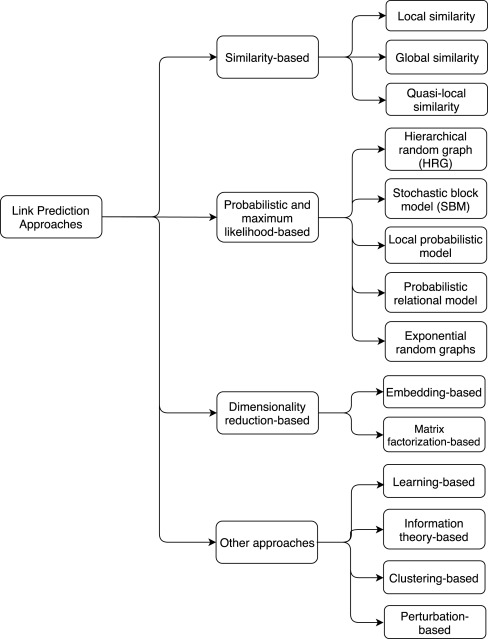
\includegraphics[width=9cm, keepaspectratio]{capitoli/methods/imgs/img2.jpg}
\end{figure}

\section{Similarity-based Methods}

Similarity-based metrics are the simplest one in link prediction, in
which for each pair \(x\) and \(y\), a similarity score \(S(x, y)\) is
calculated. The score \(S(x, y)\) is based on the structural or node's
properties of the considered pair. The non-observed links (i.e.,
\(U - E^T\) ) are assigned scores according to their similarities.
\textbf{The pair of nodes having a higher score represents the predicted
    link between them}. The similarity measures between every pair \emph{can
    be calculated using several properties of the network}, one of which is
structural property. Scores based on this property can be grouped in
several categories like \textbf{local and global}, and so on.

\subsection{Local similarity indices}

Local indices are generally calculated using information about common
neighbors and node degree. These indices \textbf{consider immediate
    neighbors of a node}. The following are some examples of local
similarity indices with a description and method to calculate them:

\begin{itemize}
    \item \texttt{Common\ Neighbors\ (CN)}: In a given network or graph, the size
          of common neighbors for a given pair of nodes \(x\) and \(y\) is
          calculated as the size of the intersection of the two nodes
          neighborhoods ( \(\Gamma\) ). \[S(x, y) = |\Gamma(x) \cap \Gamma(y)|\]
          The likelihood of the existence of a link between x and y increases with
          the number of common neighbors between them.
    \item \texttt{Jaccard\ Coefficient}: This metric is similar to the Common
          Neighbors. Additionally, it normalizes the above score, as given below:
          \[S(x, y) = \frac{|\Gamma(x) \cap \Gamma(y)|}{|\Gamma(x) \cup \Gamma(y)|}\]
          The Jaccard coefficient is defined as the probability of selection of
          common neighbors of pairwise vertices from all the neighbors of either
          vertex. The pairwise Jaccard score increases with the number of common
          neighbors between the two vertices considered. Some researcher
          (\textbf{Liben-Nowell et al.}) demonstrated that this similarity metric
          \textbf{performs worse} as compared to Common Neighbors.
    \item \texttt{Adamic/Adar\ Index\ (AA)}: Adamic and Adar presented a metric to
          calculate a similarity score between two web pages based on shared
          features, which are further used in link prediction after some
          modification
          \[S(x, y) = \sum_{z \in \Gamma(x) \cap \Gamma(y)} \frac{1}{log k_z}\]
          where \(k_z\) is the degree of the node \(z\). It is clear from the
          equation that more weights are assigned to the common neighbors having
          smaller degrees. This is also intuitive in the real-world scenario, for
          example, a person with more number of friends spend less time/resource
          with an individual friend as compared to the less number of friends.
    \item \texttt{Preferential\ Attachment\ (PA)}: The idea of preferential
          attachment is applied to generate a growing scale-free network. The term
          \textbf{growing} represents the incremental nature of nodes over time in
          the network. The likelihood incrementing new connection associated with
          a node \(x\) is proportional to \(k_x\) , the degree of the node.
          Preferential attachment score between two nodes x and y can be computed
          as: \[S(x, y) = k_x k_y\] This index shows the worst performance on most
          networks. The \textbf{simplicity} (as it requires the least information
          for the score calculation) and the \textbf{computational time} of this
          metric are the main advantages. PA shows better results if larger degree
          nodes are densely connected, and lower degree nodes are rarely
          connected. In the above equation, summation can also be used instead of
          multiplication as an aggregate function.
    \item \texttt{Resource\ Allocation\ Index\ (RA)}: Consider two non-adjacent
          vertices \(x\) and \(y\). Suppose node \(x\) sends some resources to
          \(y\) through the common nodes of both \(x\) and \(y\) then the
          similarity between the two vertices is computed in terms of
          \textbf{resources sent} from \(x\) to \(y\). This is expressed
          mathematically as:
          \[S(x, y) = \sum_{z \in \Gamma(x) \cap \Gamma(y)} \frac{1}{k_z}\] The
          difference between \textbf{RA} and \textbf{AA} is that the RA index
          heavily penalizes to higher degree nodes compared to the AA index.
          Prediction results of these indices become almost the same for smaller
          average degree networks. This index shows good performance on
          heterogeneous networks with a high clustering coefficient, especially on
          transportation networks.
    \item \texttt{Cosine\ similarity\ or\ Salton\ Index\ (SI)}: This similarity
          index between two records (documents) is measured by calculating the
          Cosine of the angle between them. The metric is all about the
          orientation and not magnitude. The Cosine similarity can be computed as
          \[S(x, y) = \frac{|\Gamma(x) \cap \Gamma(y)|}{\sqrt{(k_x k_y)}}\] -
          \texttt{Sorensen\ Index}: It is very similar to the Jaccard index.
          \textbf{McCune et al.} show that it \textbf{is more robust than Jaccard
              against the outliers}.
          \[S(x, y) = \frac{2|\Gamma(x) \cap \Gamma(y)|}{k_X + k_y}\]
    \item \texttt{CAR-based\ Common\ Neighbor\ Index\ (CAR)}: CAR-based indices
          are presented based on the assumption that the link existence between
          two nodes is more likely if their common neighbors are members of a
          local community (local-community-paradigm (LCP) theory). In other words,
          the likelihood existence increases with the number of links among the
          common neighbors (local community links (LCLs)) of the seed node pair as
          described in the following figure.
          \[S(x, y) = CN(x, y) \text{ x } LCL(x, y) = CN(x, y) \text{ x } \sum_{z \in \Gamma(x) \cap \Gamma(y)} \frac{|\gamma(z)|}{2} \]
          where \(CN(x, y) = |\Gamma(x) ∩ \Gamma(y)|\) is number of common
          neighbors. \(LCL(x, y)\) refers to the number of local community links
          which are defined as the links among the common neighbors of seed nodes
          x and y. \(\gamma(z)\) is the subset of neighbors of node \(z\) that are
          also common neighbors of \(x\) and \(y\).

          \begin{figure}[H]
              \centering
              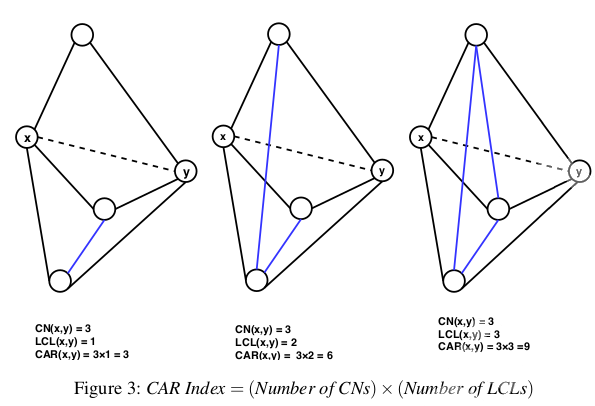
\includegraphics[width=8cm, keepaspectratio]{capitoli/methods/imgs/img3.png}
          \end{figure}
    \item \texttt{CAR-based\ Adamic/Adar\ Index\ (CAA)}: If \(LCL\) is considered
          as an accuracy enhancer, then the \(CAA\) index is obtained by
          incorporating the \(LCL\) theory to the well known AA index and
          mathematically expressed by the equation given below.
          \[S(x, y) = \sum_{z \in \Gamma(x) \cap \Gamma(y)} \frac{|\gamma(z)|}{\log_2(k_z)} \]
    \item \texttt{CAR-based\ Resource\ Allocation\ Index\ (CRA)}: Is a general
          application of the LCL theory to other indices and generate the CRA
          index by incorporating this concept into the existing RA index of the
          literature. Mathematically, the CRA can be expressed as
          \[S(x, y) = \sum_{z \in \Gamma(x) \cap \Gamma(y)} \frac{|\gamma(z)|}{k_z}\]
    \item \texttt{CAR-based\ Preferential\ Attachment\ Index\ (CPA)}: This is
          the preferential attachment index based on the CAR index. CPA is
          obtained by incorporating the LCL theory to the original PA method and
          expressed mathematically by
          \[S(x, y) = e_x e_y + e_x CAR(x, y) + e_y CAR(x, y) + CAR(x, y)^2\]
          where \(e_x\) is the number of neighbors of \(x\) not shared by \(y\)
          and \(CAR(x, y)\) is the similarity score of the node pair \(x\) and
          \(y\) using CAR index. CAR-based methods listed above show the best
          performance on LCP networks. The LCP networks are related to dynamic and
          heterogeneous systems and facilitate network evolution of social and
          biological networks.
    \item \texttt{Hub\ Promoted\ Index\ (HPI)}: This
          similarity index promotes the formation of links between the sparsely
          connected nodes and hubs. It also tries to prevent links formation
          between the hub nodes. This similarity metric can be expressed
          mathematically as
          \[S(x, y) = \frac{|\Gamma(x) \cap \Gamma(y)|}{min(k_x, k_y)}\]
    \item \texttt{Hub\ Depressed\ Index\ (HDI)}: This index is the same as the
          previous one but with the opposite goal as it avoids the formation of
          links between hubs and low degree nodes in the networks. The Hub
          depressed index promotes the links evolution between the hubs as well as
          the low degree nodes. The mathematical expression for this index is
          given below.
          \[S(x, y) = \frac{|\Gamma(x) \cap \Gamma(y)|}{max(k_x, k_y)}\]
    \item \texttt{Local\ Naive\ Bayes-based\ Common\ Neighbors\ (LNBCN)}: The
          above similarity indices are somehow based on common neighbors of the
          node pair where each of the which are equally weighted. This method is
          based on the Naive Bayes theory and arguments that different common
          neighbors play different role in the network and hence contributes
          differently to the score function computed for non-observed node pairs
          \[S(x, y) = \sum_{z \in \Gamma(x) \cap \Gamma(y)} [log(\frac{C(z)}{1 - C(z)}) + log(\frac{1 - \rho}{\rho})]\]
          where \(C(z)\) is node clustering coefficient and \(\rho\) is the
          network density expressed as \[\rho = \frac{|E|}{n(n-1)/2}\]
    \item \texttt{Leicht-Holme-Newman\ Local\ Index\ (LHNL)}: The logic below this
          index is that two vertices are similar to each other if their
          corresponding neighbors are self-similar to themselves. This score is
          defined by the ratio of the path of length two that exits between two
          vertices and the expected path of the same length between them.
          \[S(x, y) = \frac{|\Gamma(x) \cap \Gamma(y)|}{k_x k_y}\]
    \item \texttt{Node\ Clustering\ Coefficient\ (CCLP)}: This index is also based
          on the clustering coefficient property of the network in which the
          clustering coefficients of all the common neighbors of a seed node pair
          are computed and summed to find the final similarity score of the pair.
          Mathematically \[S(x, y) = \sum_{z \in \Gamma(x) \cap \Gamma(y)} C(z)\]
          where \[C(z) = \frac{t(z)}{k_z(k_z - 1)}\] is clustering coefficient of
          the node \(z\) and \(t(z)\) is the total triangles passing through the
          node \(z\).
    \item \texttt{Node\ and\ Link\ Clustering\ coefficient\ (NLC)}:
          This similarity index is based on the basic topological feature of a
          network called ''\emph{Clustering Coefficient}''. The clustering
          coefficients of both nodes and links are incorporated to compute the
          similarity score.
          \[S(x, y) = \sum_{z \in \Gamma(x) \cap \Gamma(y)} \frac{|\Gamma(x) \cap \Gamma(z)|}{k_z -1} \text{ x }C(z) + \frac{|\Gamma(y) \cap \Gamma(z)|}{k_z -1} \text{ x }C(z)\]

\end{itemize}

\subsection{Global similarity indices}

Global indices are computed using entire topological information of a
network. The computational complexities of such methods are higher and
seem to be infeasible for large networks.

\begin{itemize}
    \item \texttt{Katz\ Index}: This
          index can be considered as a variant of the shortest path metric. It
          directly aggregates over all the paths between x and y and dumps
          exponentially for longer paths to penalize them. It can be expressed
          mathematically as:
          \[S(x, y) = \sum_{l = 1}^{\infty}\beta^l|paths_{x, y}^{<l>}| = \sum_{l = 1}^{\infty}\beta^l(A)^l_{x, y}\]
          where, \(paths_{x, y}^{<l>}\) is considered as the set of total \(l\)
          length paths between \(x\) and \(y\), \(\beta\) is a damping factor that
          controls the path weights and A is the adjacency matrix. For the
          convergence of above equation, \[\beta < \frac{1}{\lambda_1} \] where
          \(\lambda_1\) is the maximum eigenvalue of the matrix A. If 1 is added
          to each element of the diagonal of the resulting similarity matrix S,
          this expression can be written in matrix terms as \[S = \beta AS + I\]
          where \(I\) is the identity matrix of the proper dimension. The
          similarity between all pairs of nodes can be directly computed using the
          closed-form by rearranging for \(S\) in the previous expression and
          subtracting the previously added 1 to the elements in the diagonal. Katz
          score for each pair of nodes in the network is calculated by finding the
          similarity matrix as \[S = (I - \beta A)^{- 1} - I\] The computational
          complexity of the given metric is high, and it can be roughly estimated
          to be cubic complexity which is not feasible for a large network.
    \item \texttt{Random\ Walk\ with\ Restart\ (RWR)}: Let \(\alpha\) be a
          probability that a random walker iteratively moves to an arbitrary
          neighbor and returns to the same starting vertex with probability
          \((1 - \alpha)\). Consider \(q_{xy}\) to be the probability that a
          random walker who starts walking from vertex \(x\) and located at the
          vertex \(y\) in steady-state. Now, this probability of walker to reach
          the vertex \(y\) is expressed mathematically as
          \[\overrightarrow{q_x} = \alpha P^T \overrightarrow{q_x} + (1-\alpha) \overrightarrow{e_x}\]
          where \(\overrightarrow{e_x}\) is the seed vector of length \(|V|\)
          (i.e., the total number of vertices in the graph). This vector consists
          of zeros for all components except the elements \(x\) itself. The
          transition matrix \(P\) can be expressed as
          \[\overrightarrow{q_x} = (1-\alpha)(I - \alpha P^T)^{-1} \overrightarrow{e_x}\]
          Since this similarity is not symmetric, the final score between the node
          pair (x, y) can be computed as \[S(x, y) = q_{xy} + q_{yx}\] It is clear
          from the above equation that matrix inversion is required to solve,
          which is quite expensive and prohibitive for large networks.
    \item \texttt{Shortest\ Path}: The inverse relation between the similarity and
          length of the shortest path is captured by the following mathematical
          equation given below. \[S(x, y) = -|d(x, y)|\] where Dijkstra algorithm
          is applied to efficiently compute the shortest path d(x, y) between the
          node pair (x, y). The prediction accuracy of this index is low compared
          to most local indices.
    \item \texttt{Leicht-Holme-Newman\ Global\ Index\ (LHNG)}: This global index
          is based on the principle that two nodes are similar if either of them
          has an immediate neighbor, which is similar to the other node. This is a
          recursive definition of similarity where a termination condition is
          needed. The termination condition is introduced in terms of
          self-similarity, i.e., a node is similar to itself. Thus, the similarity
          score equation consists of two terms: first, the neighbor similarity,
          and the second, self-similarity, as given below.
          \[S(x, y) = \phi  \sum_z A_{x, z} S_{z, y} + \psi \delta_{x, y}\] Here,
          the first term is neighborhood similarity and the second term is
          self-similarity. \(\psi\) and \(\phi\) are free parameters that make a
          balance between these two terms. When the free parameter \(\psi\) = 1,
          this index resembles to the Katz index.
    \item \texttt{Cosine\ based\ on\ L+\ (Cos+)}: Laplacian matrix is extensively
          used as an alternative representation of graphs in spectral graph
          theory. This matrix can be defined as \(L = D - A\), where, \(D\) is the
          diagonal matrix consisting of the degrees of each node of the matrix and
          \(A\) is the adjacency matrix of the graph. The pseudo-inverse of the
          matrix defined by Moore-Penrose is represented as \(L^+\) and each entry
          of this matrix is used to represent the similarity score between the two
          corresponding nodes. The most common way to compute this pseudo-inverse
          is by computing the \textbf{singular value decomposition (SVD)} of the
          Laplacian matrix [$(L = U \Sigma V^{}T)$, where \(U\) and \(V\)
                  are left and right singular vectors of \(SVD\)] as follows
          \[L^+ = V \Sigma^+ U^T\] \(\Sigma^+\) is obtained by taking the inverse
          of each nonzero element of the \(\Sigma\). Further, the similarity
          between two nodes \(x\) and \(y\) can be computed using any inner
          product measure such as Cosine similarity given as
          \[S(x, y) = \frac{L_{x, y}^+}{\sqrt{L_{x, x}^+ L_{y, y}^+}}\]
    \item \texttt{Average\ Commute\ Time\ (ACT)}: This index is based on the
          random walk concept. A random walk is a Markov chain which describes the
          movements of a walker. It defined as the average number of
          movements/steps required by a random walker to reach the destination
          node \(y\), and come back to the starting node \(x\). If \(m(x, y)\) be
          the number of steps required by the walker to reach \(y\) from \(x\),
          then the following expression captures this concept.
          \[n(x, y) = |E| (l_{xx}^+ + l_{yy}^+ - 2l_{xy}^+) \] where \(l_{xy}^+\)
          denotes the \((x, y)\) entry of the matrix \(L^+\) . Pseudo-inverse of
          the Laplacian, \(L^+\) can be computed as
          \[L^+ = (L - \frac{ee^T}{n})^{-1} + \frac{ee^T}{n}\] where \(e\) is a
          column vector consisting of 1's. Smaller value of this equation will
          represent higher similarity. The final expression is the following
          \[S(x, y) = \frac{1}{l_{xx}^+ + l_{yy}^+ - 2l_{xy}^+}\]
    \item \texttt{Normalized\ Average\ Commute\ Time\ (NACT)}: This is a variant
          of ACT that takes into account node degrees. For a high degree node
          (hub) \(y\), \(m(x, y)\) is usually small regardless of \(x\), the
          similarity measure is normalized with stationary distribution \(\pi\) of
          the Markov chain describing random walker on the graph. This normalized
          measure can be computed with the following equation
          \[S(x, y) = \frac{1}{(m(x, y)\pi_y + m(y, x)\pi_x)}\]
    \item \texttt{Matrix\ Forest\ Index\ (MF)}: his index is based on the concept
          of spanning tree which is defined as the subgraph that spans total nodes
          without forming any cycle. The spanning tree may contain total or less
          number of links as compared to the original graph. Chebotarev and Shamis
          proposed a theorem called matrix-forest theorem which states that the
          number of spanning tree in a graph is equal to the co-factor of any
          entry of Laplacian matrix of the graph. Here, the term forest represents
          the union of all rooted disjoint spanning trees. The similarity between
          two nodes \(x\) and \(y\) can be computed with the equation given below
          \[S = (I + L)^{-1}\] where \((I + L)\_{(x,y)}\) is the number of
          spanning rooted forests ( \(x\) as root ) consisting of both the nodes
          \(x\) and \(y\). Moreover, this quantity is equal to the co-factor of
          \((I + L)_{(x,y)}\) .
    \item \texttt{SimRank}: This is a measure of
          structural context similarity and shows object-to-object relationships.
          It is not domain-specific and recommends to apply in directed or mixed
          networks. The basic assumption of this measure is that two objects are
          similar if they are related to similar objects. SimRank computes how
          soon two random walkers meet each other, starting from two different
          positions. This measure can be represented in matrix form as
          \[S(x,y) = \alpha W^T SW + (1 - \alpha)I\] where, \(\alpha \in (0, 1)\)
          is a constant. \(W\) is the transformation matrix and computed by
          normalizing each column of adjacency matrix \(A\) as
          \[
              W_{ij} = \frac{a_{ij}}{\sum_{k=1}^{n}}
          \]
          The computational complexity
          of this measure is high for a large network, and to reduce its time, the
          authors suggest pruning recursive branches.
    \item \texttt{Rooted\ Pagerank\ (RPR)}: The idea of PageRank was originally
          proposed to rank the web pages based on the importance of those pages.
          The algorithm is based on the assumption that a random walker randomly
          goes to a web page with probability \(\alpha\) and follows hyper-link
          embedded in the page with probability \((1 - \alpha)\). Chung et
          al.~used this concept incorporated with a random walk in link prediction
          framework. The importance of web pages, in a random walk, can be
          replaced by stationary distribution. The similarity between two vertices
          \(x\) and \(y\) can be measured by the stationary probability of \(y\)
          from \(x\) in a random walk where the walker moves to an arbitrary
          neighboring vertex with probability \(\alpha\) and returns to \(x\) with
          probability \((1 - \alpha)\). Mathematically, this score can be computed
          for all pair of vertices as
          \[RPR = (1 - \alpha)(I - \alpha \hat{N})^{-1}\] where
          \(\hat{N} = D^{-1} A\) is the normalized adjacency matrix with the
          diagonal degree matrix \(D[i, i] = \sum_j A[i, j]\).
\end{itemize}

\subsection{Quasi-local indices}

Quasi-local indices have been introduced as a trade-off between local
and global approaches or performance and complexity. These metrics are
as efficient to compute as local indices. Some of these indices extract
the entire topological information of the network. The time complexities
of these indices are still below compared to the global approaches.

\begin{itemize}
    \item \texttt{Local\ Path\ Index\ (LP)}: This metric has the intent to furnish
          a good trade-off between accuracy and computational complexity. The
          metric is expressed mathematically as \[S^{LP} = A^2 + \epsilon A^3\]
          where $\epsilon$ represents a free parameter. Clearly, the measurement
          converges to common neighbor when \(\epsilon = 0\). If there is no
          direct connection between \(x\) and \(y\), \((A^3)_{xy}\) is equated to
          the total different paths of length 3 between \(x\) and \(y\). The index
          can also be expanded to generalized form
          \[S^{LP} = A^2 + \epsilon A^3 + \epsilon^2 A^4 + ... + \epsilon^{(n−2)} A^n\]
          where \(n\) is the maximal order. Computing this index becomes more
          complicated with the increasing value of \(n\). The LP index outperforms
          the proximity-based indices, such as RA, AA, and CN.
    \item \texttt{Path\ of\ Length\ 3\ (L3)}: Georg Simmel, a German sociologist,
          first coined the concept ``triadic closure'' and made popular by Mark
          Granovetter in his work ``\emph{The Strength of Weak Ties}''. The
          authors proposed a similarity index in protein-protein interaction (PPI)
          network, called \textbf{\emph{path of length 3 (or L3)}} published in
          the Nature Communication. They experimentally show that the triadic
          closure principle (TCP) does not work well with PPI networks. They
          showed the paradoxical behavior of the TCP (i.e., the path of length 2),
          which does not follow the structural and evolutionary mechanism that
          governs protein interaction. The TCP predicts well to the interaction of
          self-interaction proteins (SIPs), which are very small (4\%) in PPI
          networks and fails in prediction between SIP and non SIP that amounts to
          96\%. They showed that the L3 index performs well in such conditions and
          give mathematical expression to compute this index as
          \[S(x, y) = \sum \frac{a_{x,u} a_{u,v} a_{v,y}}{k_u k_v}\]
    \item \texttt{Similarity\ based\ on\ Local\ Random\ Walk\ and\ Superposed\ Random\ Walk\ (LRW\ and\ SRW)}:
          This metric propose a new similarity measures by exploiting the random
          walk concept on graphs with limited walk steps. They defined node
          similarity based on random walks of lower computational complexity
          compared to the other random walk based methods. Given a random walker,
          starting from the node \(x\), the probability of reaching the random
          walker to the node \(y\) in \(t\) steps is
          \[\overrightarrow{\pi}\_x(t) = P^T \overrightarrow{\pi}\_x(t-1)\] where
          \(\overrightarrow{\pi}\_x(0)\) is a column vector with \(x^{th}\)
          element as 1 while others are 0's and \(P^T\) is the transpose of the
          transition probability matrix \(P\). \(P_{xy}\) entry of this matrix
          defines the probability of a random walker at node \(x\) will move to
          the next node \(y\). It is expressed as \(P_{xy} = \frac{a_{kx}}{k_x}\)
          , where \(a_{xy}\) is 1 when there is a link between \(x\) and \(y\) and
          0, otherwise. The authors computed the similarity score ( \(LRW\) )
          between two nodes based on the above concept as
          \[S^{LRW}(x, y) = \frac{k_x}{2|E|}\pi_{xy}(t) + \frac{k_y}{2|E|}\pi_{xy}(t)\]
          This similarity measure focus on only few steps covered by the random
          walker (hence quasi-local) and not the stationary state compared to
          other approaches. Random walk based methods suffer from the situation
          where a random walker moves far away with a certain probability from the
          target node whether the target node is closer or not. This is an obvious
          problem in social networks that show a high clustering index i.e.,
          clustering property of the social networks. This degrades the similarity
          score between the two nodes and results in low prediction accuracy. One
          way to counter this problem is that continuously release the walkers at
          the starting point, which results in a higher similarity between the
          target node and the nearby nodes. By superposing the contribution of
          each walker (walkers move independently), SRW is expressed as
          \[S^{SRW} (x, y) (t) = \sum_{l=1}^{t} S^{LRW} (l)\]
\end{itemize}

\subsection{Some Remarks}

Similarity-based approaches mostly focus on the structural properties of
the networks to compute the similarity score. \textbf{\emph{Local
        approaches}} consider, in general, neighborhood information (direct
neighbors or neighbors of neighbor), which take less time for
computation. This is the property that makes the local approaches
feasible for massive real-world network datasets. \textbf{\emph{Global
        approaches}} consider the entire structural information of the network;
that is why time required to capture this information is more than local
and quasi-local approaches. Also, sometimes, entire topological
information may not be available at the time of computation, especially
in a decentralized environment. So, parallelization over the global
approaches may not possible or very complex compared to the local and
quasi-local approaches. The performance or prediction accuracy of these
approaches (i.e., global approaches) is better compared to local and
quasi-local. \textbf{\emph{Quasi-local approaches}} extract more
structural information than local and somehow less information compared
to the global.


\section{Probabilistic and maximum likelihood models}

For a given network \(G(V, E)\), \textbf{\emph{the probabilistic model
        optimizes an objective function to set up a model that is composed of
        several parameters}}. Observed data of the given network can be
estimated by this model nicely. At that point, the likelihood of the
presence of a non-existing link \((i, j)\) is evaluated using
conditional probability \(P(A_{i j} = 1 | \Theta )\). Several
\texttt{probabilistic\ models} and \texttt{maximum\ likelihood\ models}
have been proposed in the literature to \textbf{infer missing links in
    the networks}.\\

\textbf{The probabilistic models normally require more information like
    node or edge attribute knowledge in addition to structural information}
Extracting these attribute information is not easy; moreover, the
parameter tuning is also a big deal in such models that limit their
applicability. \emph{Maximum likelihood methods are complex and
    time-consuming}, so these models are not suitable for real large
networks.

\subsection{Local probabilistic model for link prediction}

\textbf{Wang et al.} proposed a \texttt{local\ probabilistic\ model} for
link prediction in an \emph{undirected network}. They employed three
different types of features viz., topological, semantic, and
cooccurrence probability features extracted from different sources of
information.\\

They presented an idea of a central neighborhood set derived from the
local topology of the considered node-pair, which is relevant
information for the estimation of a link between them. They computed
non-derivable frequent itemsets (i.e., those itemsets whose occurrence
statistics can not be derived from other itemset patterns) from the
network events log data, which is further used as training data for the
model. An event corresponds to a publication of a paper (i.e., authors'
interactions in the paper is a an event, and a set of such events is the
event log) in the Coauthorship network. The model is shown in the
following Figure, which considers the approach described below.\\

First, the central neighborhood set between \(x\) and \(y\) is
calculated based on local event log data. One of the usual ways to find
the central neighborhood set is to find the \textbf{shortest path
    between two vertices of specified length}, and the vertices are lying on
this path can be included in the required set. There can be more than
one shortest path between two vertices, so more neighborhood sets can be
possible. Neighborhood sets of shorter lengths and more frequent
(frequency score is used when more shortest paths of the same length are
available) are chosen for the central neighborhood set. The authors
considered the shortest path up to length 4 since the nodes lying on the
shorter length path are more relevant.\\

In the second step, for a given central neighborhood set, non-derivable
frequent itemsets are used to learn the local probabilistic model.
\textbf{Calders et al.} proposed a depth-first search method to
calculate non-derivable itemsets and the same algorithm used by the
authors. Why non-derivable frequent itemsets? \textbf{Pavlov et al.}
first introduced the concept of frequent itemset to construct an
\texttt{MRF}. They argued that a \(K-itemset\) and its support
represents a \(K-way\) statistics, which can be viewed as a constraint
on the true underlying distribution that generates the data. Given a set
of itemset constraints, a maximum entropy distribution satisfying all
these constraints is selected as the estimate for the true underlying
distribution. This maximum entropy distribution is equivalent to an
\texttt{MRF}. Since the number formed links are very few compared to all
possible links in a sparse network, the authors used a support threshold
of one to extract all frequent itemsets. Theses extracted itemsets are
large in number that results in expensive learning for the \texttt{MRF}.
To reduce this cost, only non-derivable itemsets are extracted. They
find all such itemsets that lie entirely within the central neighborhood
set. Using these itemsets, a \texttt{Markov\ Random\ Field} is
\textbf{learned}.\\

In the last step, the \texttt{iterative\ scaling\ algorithm} is used to
learn a local \texttt{MRF} for the given central neighborhood set. This
process continues overall itemset constraints and continuously updates
the model until the model converges. Once the model learning process is
over, one can infer the co-occurrence probability by computing the
marginal probability over the constructed model. The
\texttt{Junction\ tree\ inference\ algorithm} is used to infer
co-occurrence probability. The algorithm to induce co-occurrence
probability feature for a pair of vertices can be found in
\href{https://static.aminer.org/pdf/PDF/000/303/209a_parameterized_probabilistic_model_of_network_evolution_for_supervised_link.pdf}{Local
    Probabilistic Models for Link Prediction}.

\subsection{Probabilistic relational model for link prediction (PRM)}

Existing works show that \textbf{node attributes play a significant role
    to improve the link prediction accuracy}. However, \textbf{no generic
    framework is available to incorporate node and link attributes} and
hence, not applicable to all scenarios. To this end, \textbf{the
    probabilistic model is a good and concrete solution that provides a
    systematic approach to incorporate both node and link attributes in the
    link prediction framework}. Pioneering works on \texttt{PRM} include
\textbf{Getoor et al.} study on directed networks, \textbf{Taskar et
    al.} study on undirected networks, \textbf{Jennifer Neville}
work on for both networks, etc. published in \texttt{JMLR} is based on
\texttt{Relational\ Bayesian\ network\ (RBN)} where relation links are
directed and published in NIPS is based on
\texttt{Relational\ Markov\ network\ (RMN)} where relational links are
undirected.\\

\texttt{PRM} was originally designed for attribute prediction in
relational data, and it later extended to link prediction task. The
authors employed the attribute prediction framework to link prediction.
This casting can be understood with the following example: - Consider
the problem of link prediction in a coauthorship network. Non-relational
frameworks of link prediction consider only one entity type
``\emph{person}'' as node and one relationship; however, relational
framework (\texttt{PRMs}) include more entity types like article,
conference venue, institution, etc. Each entity can have attributes like
a person (attributes: name, affiliation institute, status (student,
professor)), article (attributes: publication year, type (regular,
review)), etc. Several relational links may possible among these
entities like advisor-advisee/research scholar relation between two
persons, author relationship between person and paper entities, and
paper can be related to the conference venue with publish relationship.
Moreover, relationships (links) among these entities can also have
attributes viz., exists (if there is a link between the two involved
entities), or not-exist (no link between the involved entities). This
way, the link prediction can be reduced to an attribute prediction
framework/model.\\

During the model training, a single link graph is constructed that
incorporates above heterogeneous entities and relationships among them.
Model parameters are estimated discriminatively to maximize the
probability of the link existence and other parameters with the given
graph attribute information. The learned model is then applied using
probabilistic inference to predict missing links.\\

\subsection{Hierarchical structure model (HSM)}

These models are based on the assumption that the structures of many
real networks are hierarchically organized, where nodes are divided into
groups, which are further subdivided into subgroups and so forth over
multiple scales. Some representative work systematically encodes such
structures from network data to build a model that estimates model
parameters using statistical methods. These parameters are then used in
estimating the link formation probability of unobserved links.\\

Some studies suggest that many real networks, like biochemical networks
(protein interaction networks, metabolic networks, or genetic regulatory
networks), Internet domains, etc. are hierarchically structured. In
hierarchical networks, vertices are divided into groups, which are
further sub-divided into subgroups and so forth over multiple scales.
\textbf{Clauset et al.} proposed a probabilistic model that takes a
hierarchical structure of the network into account. The model infers
hierarchical information from the network data and further applies it to
predict missing links.\\

The hierarchical structures are represented using a tree (binary), or
dendrogram, where, the leaves (i.e., \(n\) ) represent the number of
total vertices in the network and each internal vertex out of (
\(n - 1\) ) corresponds to the group of vertices descended from it. Each
internal vertex \(r\) is associated with a probability \(p_r\) , then
the existing edge probability \(p_{xy}\) between two vertices \(x\) and
\(y\) is given by \(p_{xy} = p_r\) where, \(r\) is their lowest common
ancestor. The hierarchical random graph is then, represented by the
dendrogram \(D^{\star}\) with the set of probability \(\{ p_r \}\) as
\(\left( D^{\star},\{p_r\} \right)\). Now the learning task is to find
the hierarchical random graph(s) that best estimates the observed
real-world network data. Assuming all possible dendrograms to be equally
likely, Bayes theorem says that the probability of the dendrogram
\(\left(D^{\star}, \{p_r\} \right)\) that best estimates the data is
proportional to the posterior probability or likelihood, \(L\) from
which the model generates the observed network and our goal is to
maximize \(L\) . The likelihood of a hierarchical random graph
\(\left(D^{\star},\{p_r\} \right)\) is computed using the following
equation

\[
    L(D^{\star}, \{p_r\}) = \prod_{r \in D^{\star}} p_r^{E_r} (1-p_r)^{L_r R_r - Er},
\]

where \(L_r\) and \(R_r\) are the left and right subtree rooted at
\(r\), and \(E_r\) is the number of links in the network whose endpoints
have \(r\) as their lowest common ancestor in \(D^{\star}\) . The above
equation assumes the convention \(0^0 = 1\). For a given dendrogram
\(D^{\star}\) , it is easy to compute the probability \(p_r\) that
maximizes \(L(D^{\star}, \{p_r\})\) i.e.

\[
    \overline{p_r} = \frac{E_r}{L_r R_r}.
\]

This can be understood with the following example illustrated in the
next Figure. Now, this model can be used to estimate the missing links
of the network as follows. Sample a large number of dendrograms with
probability proportional to their likelihood. Then, compute the mean
connecting probability \(\overline{p_{xy}}\) of each nonexisting pair
\((x, y)\) by averaging the corresponding probability \(p_{xy}\) overall
sampled dendrograms. Sort these vertices pairs scores in descending
order and selects top-l links to be predicted.

\begin{figure}[H]
    \centering
    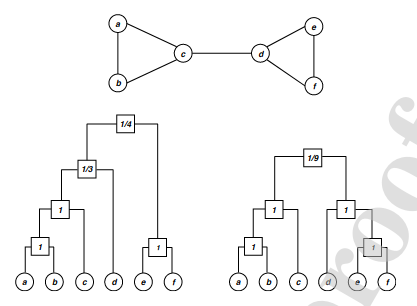
\includegraphics[width=8cm, keepaspectratio]{capitoli/methods/imgs/img8.png}
    \caption{ An illustrating example of \texttt{HSM} for a graph of 6 nodes and its
        two possible dendrograms. The internal nodes of each dendrogram are
        labeled as the maximum likelihood probability \(\overline{p}_r\). The
        likelihoods of the left and the right dendrograms are
        \(L(D1) = (1/3)(2/3)^2 (1/4)^2(3/4)^6\) \(= 0.00165\), and
        \(L(D2) = (1/9)(8/9)^8 = 0.0433\). Thus, the second (i.e., right)
        dendrogram is most probable as it divides the network in a balanced one
        at the first level.}
\end{figure}

\subsection{Stochastic block model (SMB)}

Hierarchical structures may not represent most networks. A more general
approach to represent these networks is block model where vertices are
distributed (partitioned) into blocks or communities and the connecting
probability between two vertices depends on blocks they belong to.
\textbf{Guimera et al.} presented a novel framework where stochastic
block model representation of a network is employed to find missing and
spurious links. The authors compute the reliability of the existence of
links given an observed network that is further used to find missing
links (non-existing links with higher reliabilities) and spurious links
(existing links with lower probabilities).\\

The link reliability \(R_{xy}\) between the two vertices \(x\) and \(y\)
is

\[R_{xy} = p_{BM} (A_{xy} = 1 | A^0).\]

i.e.~probability that the link truly exists given the observed network
\(A^0\), the block model \(BM\).\\

Generally, complex networks are outcomes of combination of mechanisms,
including modularity, role structure, and other factors. In \(SBM\),
partitioning vertices of network based on these mechanisms may result in
different block models that capture different correlations (patterns) of
the network. Assume that no prior knowledge of suitable models, the
reliability is expressed as

\[
    R_{xy} = \frac{1}{Z} \sum_{P \in P^{\star}} \left( \frac{l^{0}_{\sigma_x \sigma_y} + 1}{r^{0}_{\sigma_x \sigma_y + 2}} \right) \text{ exp } \left[ -H(P) \right],
\]

where the sum is over all possible partitions \(P^{\star}\) of the
network into groups, \(\sigma_x\) and \(\sigma_y\) are vertices \(x\)
and \(y\) groups in partition \(P\) respectively. Moreover, \(l^0_1\)
and \(r^0_{\sigma_{\alpha} \sigma_{\beta}}\) are the number of links and
maximum possible links in the observed network between groups \(\alpha\)
and \(\beta\) . The function \(H(P)\) is

\[H(P) = \sum_{\alpha \leq \beta} \left[ \ln \left( r_{\alpha \beta} \right) + \ln \binom {r_{\alpha \beta}}{l^0_{\alpha \beta}} \right],\]

and \(Z = \sum_{P \in P^{\star}} \text{ exp } \left[ -H(P) \right]\).\\

Practically, solving equation \(R_{xy} = \ldots\) , i.e., summing over
all possible partitions is too complex even for a small network.
However, the Metropolis algorithm can be used to correctly sample the
relevant partitions and obtain link reliability estimates.\\

The authors employed the link reliability concept to find missing links
and to identify the spurious link in the networks with the following
procedure.

\begin{itemize}
    \item
          \((i)\) Generate the observed network \(A^0\) by removing/adding some
          random links (for finding missing/spurious links) from/to the true
          network \(A^t\) .
    \item
          \((ii)\) Compute the link reliability for non-observed links (i.e.
          non-existing \(+\) missing/spurious links).
    \item
          \((iii)\) Arrange these links with their reliability score in
          decreasing order and decide the top-l links as desired ones (i.e.,
          missing/spurious links).
\end{itemize}

Probabilistic and maximum likelihood methods extract useful features and
valuable correlation among the data using hierarchical and stochastic
block models, which result in significant improvements in prediction
results as compared to some similarity-based methods. However, these are
\textbf{quite complex and time-consuming even on small datasets} that
limit their applicability on large scale real-world network datasets.

\subsection{Exponential random graph model (ERGM) or P-star model}

\section{Link prediction using Dimensionality Reduction}

The curse of dimensionality is a well-known problem in machine learning.
Some researchers employ dimension reduction techniques to tackle the
above problem and apply it in the \textbf{link prediction} scenario.

\subsection{Embedding-based link prediction}

The network embedding is considered as a dimensionality reduction
technique in which higher \(D\) dimensional nodes (vertices) in the
graphs are mapped to a lower \(d\) (\(d << D\)) \textbf{dimensional
    representation (embedding)} space by preserving the node neighborhood
structures. In other words, \textbf{\emph{find the embedding of nodes to
        a lower d-dimensions such that similar nodes (in the original network)
        have similar embedding (in the representation space)}}.\\ In the Figure
below you can see an application example of a dimensionality reduction
technique to a graph that represent a social network.

\begin{figure}[H]
    \centering
    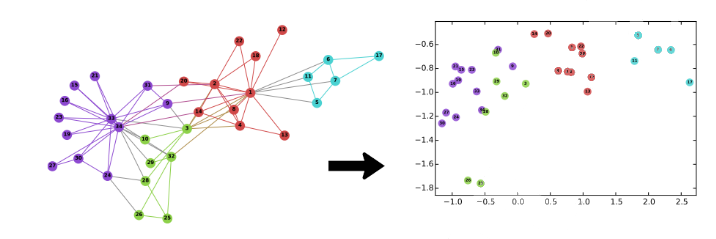
\includegraphics[width=12cm, keepaspectratio]{capitoli/methods/imgs/img4.png}
\end{figure}

The main component of the network embedding is the encoding function or
encoder \(f_{en}\) that map each node to the embedding space
\[f_{en}(x) = z_x\] where \(z_x\) is the \(d\)-dimensional embedding of
the node \(x\). The embedding matrix is \(Z \in R^{d x |V|}\), each
column of which represents an embedding vector of a node.\\

\begin{figure}[H]
    \centering
    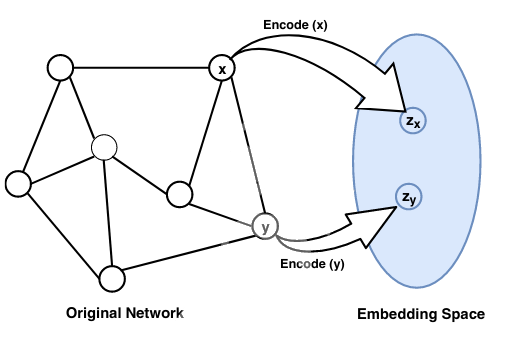
\includegraphics[width=10cm, keepaspectratio]{capitoli/methods/imgs/img5.png}
\end{figure}

Now, a similarity function is \(S(x, y)\) is defined that specifies how
to model the vector (embedding) space relationships equivalent to the
relationships in the original network, i.e.,
\[S(x, y) \approx z_x^T z_y\]

Here \(S(x, y)\) is the function that reconstructs pairwise similarity
values from the generated embedding. The term \(S(x, y)\) is the one
that differ according to the function used in different
factorization-based embedding approaches.\\

For example, \texttt{graph\ factorization} directly employ adjacency
matrix \(A\) i.e.~\((S(x, y) \overset{\Delta}{=} A_{(x,y)})\) to capture
first order proximity, \texttt{GraRep} selects
\((S(x, y) \overset{\Delta}{=} A^2_{(x,y)})\) and \texttt{HOPE} uses
other similarity measures(e.g. Jaccard neighborhood overlap). Most
embedding methods realize the reconstruction objective by minimizing the
loss function, L
\[L = \sum_{(x, y) \in \{V x V \}} l(z_x^T z_y, S(x, y))\]

Once the previous equation is \textbf{converged}
(i.e.~\textbf{trained}), one can use the trained encoder to generate
nodes embedding, which can further be employed to infer missing link and
other downstream machine learning tasks.\\

Recently, some network embedding techniques have been proposed and
applied successfully in link prediction problem. The
\texttt{Laplacian\ eigenmaps},
\texttt{Logically\ linear\ embedding\ (LLE)}, and \texttt{Isomap} are
examples based on the simple notion of embedding. Such embedding
techniques are having quite complex in nature and face scalability
issues. To tackle the scalability issue, graph embedding techniques have
leveraged the sparsity of real-world networks. For example,
\texttt{DeepWalk} extracts local information of truncated random walk
and embeds the nodes in representation space by considering the walk as
a sentence in the language model. It preserves higher order proximity by
maximizing the probability of co-occurrence of random walk of length
\(2k + 1\) (previous and next \(k\) nodes centered at a given node).
\texttt{Node2vec} also uses a random walk to preserves higher order
proximity but it is biased which is a trade-off between the
\texttt{breadth-first\ search\ (BFS)} and
\texttt{depth-first\ search\ (DFS)}.\\

The experimental results show that the \texttt{Node2vec} performs better
than the \texttt{Deepwalk}.\\

In next step, \textbf{Trouillon et al.} introduced complex embedding in
which simple matrix and tensor factorization have been used for link
prediction that uses a vector with complex values. Such composition of
complex embedding includes all possible binary relations especially
symmetric and anti-symmetric relations. Recently, some more studies have
been published in link prediction using embedding, for example,
\textbf{Cao et al.~subgraph embedding}, \textbf{Li et al.~deep dynamic
    network embedding}, \textbf{Kazemi et al.}, etc.

\subsection{Matrix factorization/decomposition-based link prediction}

From last decade, matrix factorization has been used in lots of papers
based on link prediction and recommendation systems. Typically, the
latent features are extracted and using these features, each vertex is
represented in latent space, and such representations are used in a
supervised or unsupervised framework for link prediction. To further
\textbf{improve the prediction results, some additional node/link or
    other attribute information can be used}. In most of the works,
non-negative matrix factorization has been used. Some authors also
applied the singular value decomposition technique. Let the input data
matrix is represented by \(X = (x_1, x_2, ..., x_n)\) that contains
\(n\) data vectors as columns. Now, factorization of this matrix can be
expressed as \[X \approx FG^T\] where
\(X \in R^{p x n}, F \in R^{p x k} , and G \in R^{n x k}\) . Here, \(F\)
contains the bases of the latent space and is called the basis matrix.
\(G\) contains combination of coefficients of the bases for
reconstructing the matrix \(X\) , and is called the coefficient matrix.
\(k\) is the dimension of latent space \((k < n)\). Several well-known
matrix factorizations are expressed based on some constraints on either
of the three matrices, for example

\begin{itemize}
    \item \texttt{SVD}:
          \(X_\pm \approx F_\pm G_\pm^T\)
    \item \texttt{NMF}:
          \(X_+ \approx F_+ G_+^T\)
    \item \texttt{Semi-NMF}:
          $X_\pm \approx F_\pm G_+\^{T} $
    \item \texttt{Convex-NMF}:
          $X_\pm \approx  X_\pm W_+ G_\pm^{T}$
\end{itemize}

In the above four equations, \(Z_\pm\) represents the nature of the
entries in the matrix \(Z\), i.e.~both positive and negative entries
allowed in the matrix \(Z\). In the last equation, \(F = XW\) represents
the convex combinations of the columns of \(F\) . Generally, such a
factorization problem can be modeled as the following
\texttt{Frobenius\ norm\ optimization\ problem}
\[min_{f, g} ||X - FG^T||^2_{fro}\]
\[\text{subject to} F \ge 0, G \ge 0\] Here \(||Z||^2_{fro}\) is the
frobenius norm of \(Z\) and the constraints represent NMF factorization.
However, any of the above four constraints can be used depending on the
requirement of the problem underlying. After solving the above
optimization problem, the similarity between a non-existing pair
\((x, y)\) can be computed by the similarity of the \(x^{th}\) and
\(y^{th}\) row vectors in the coefficient matrix \(G\).

\begin{itemize}
    % \tightlist
    \item
          \texttt{Acar\ et\ al.} expressed temporal link prediction as a matrix
          completion problem and solve it through the
          \texttt{matrix\ and\ tensor\ factorization}. They proposed a weighted
          method to collapsed the temporal data in a single matrix and factorize
          it using \texttt{CANDECOMP/PARAFAC\ (CP)} tensor decomposition method.
    \item
          \texttt{Ma\ et\ al.} also applied matrix factorization to temporal
          networks where features of each network are extracted using
          \texttt{graph\ communicability} and then collapsed into a single
          feature matrix using \texttt{weighted\ collapsing\ tensor\ (WCT)}.
          They showed the equivalence between eigen decomposition of
          \texttt{Katz\ matrix} and
          \texttt{non-negative\ matrix\ factorization\ (NMF)} of the
          communicability matrix that serves as the foundation of their
          framework.
    \item
          \texttt{Menon\ et\ al.} proposed a work for structural link
          prediction. Here, the problem is modeled as
          \texttt{matrix\ completion\ problem}, and
          \texttt{matrix\ factorization} are used to solve it. They introduced a
          supervised matrix decomposition framework that learns latent
          (unobserved) structural features of the graph and incorporates it with
          additional node/link explicit feature information to make a better
          prediction. Additionally, they allowed the factorization model to
          solve class imbalance problem by optimizing ranking loss.
    \item
          \texttt{Chen\ et\ al.} proposed a work, where the authors extracted
          topological matrix and attribute matrix and factorized these matrices
          using \texttt{non-negative\ matrix\ factorization}. The final score
          matrix is obtained by integrating these two matrices in the latent
          space.
\end{itemize}
\section{Other approaches}

\subsection{Learning-based frameworks for link prediction}

Earlier described approaches (e.g., similarity and probabilistic
methods) deal with the computing a score of each non-observed link
either by a similarity or a probabilistic function. However, \textbf{the
    link prediction problem can also be modeled as a learning-based model}
to exploit graph topological features and attribute information. The
problem is cast as a \textbf{supervised classification model} where a
\textbf{point} (i.e., training data) \textbf{corresponds to a
    vertex-pair in the network}, and the \textbf{label} of the point
\textbf{represents the presence or absence of an edge (link) between the
    pair}.\\ In other words, \emph{consider a vertex-pair} \(\mathit{(x, y)}\)
\emph{in the graph} \(\mathit{G(V, E)}\) \emph{and the label of the
    corresponding data point in the classification model is}
\(\mathit{l_{(x,y)}}\) . Then,

\[l_{(x, y)}=
    \begin{cases}
        +1 \ \text{ if } (x, y) \in E \\
        -1 \ \text{ if } (x, y) \notin E
    \end{cases}
\]

\textbf{This is typically a binary classification task} where several
classifiers (e.g.,
\texttt{decision\ tree,\ naive\ Bayes,\ support\ vector\ machine}, etc.)
can be employed to predict the label of unknown data points
(corresponding to missing links in the network). One of the major
challenges of this model (i.e., machine learning) is the
\textbf{selection of appropriate feature set}. Majority of the existing
research works extract feature sets from the network topology (i.e.,
topological information of the network). These \textbf{features are
    generic} and domain-independent that are \textbf{applicable to any
    network}. Such features are typical,
\texttt{neighborhood,\ and\ path-based\ features}.\\ Some other works
concentrate on extracting node and edge features that play a crucial
role to improve the performance of link prediction. The cost of
extraction of such features is cheap and easy, while the main
disadvantage is the domain-specific nature of them.

\subsection{Information theory-based link prediction}

Several complex networks have utilized the concept of
\textbf{information theory to compute their complexity on different
    scales}. They defined several correlation measures and modeled some
networks (e.g., \texttt{star,\ tree,\ lattice,\ ER\ graph}, etc.).
\textbf{Bauer et al.} used the \texttt{maximum\ entropy\ principle} to
assign a statistical weight to any graph and introduced random graph
construction with arbitrary degree distribution.\\

\textbf{Tan et al.} posed the link prediction problem in the
\texttt{framework\ of\ information\ theory}. They mainly focus on local
assortativity to capture local structural properties of the network and
showed that \texttt{mutual\ information\ (MI)} method performs well on
both low and highly correlated networks. Motivated by, \textbf{Zhu, B.
    and Xia} added more local features (i.e., links information of neighbors
of the seed nodes as well as their common neighbors) in their framework
and called it as \texttt{neighbor\ set\ information\ (NSI)\ index}.
Thus, they showed that the different features could be combined in an
information-theoretic model to improve the link prediction accuracy.\\

\textbf{Xu et al.} considered path entropy as a similarity metric for
the link prediction problem. The authors assumed that there is no
correlation among the degrees of the nodes in the network. Consider the
following notations based on their paper: \(L^0_{xy}\) shows no link
exists between two vertices \(x\) and \(y\), and the corresponding
existence is represented by \(L^1_{xy}\). Probability of existence of a
link between the above two vertices is given as

\[
    P(L^1_{xy}) = 1 - P(L^0_{xy}) = 1 - \frac{C^{k_y}_{M-k_x}}{C^{k_y}_M}
\]

where \(C_M^{k_Y}\) represents the number of candidate link sets for the
vertex \(y\) with all links incident with \(y\) and \(C^{k_y}_{M-k_x}\)
denotes the number of candidate link sets for the vertex \(y\) with all
links incident with \(y\) but none of them is incident with \(x\).
Outcome results on several networks demonstrate that the similarity
index based on path entropy performs better than other indices in terms
of prediction accuracy and precision. \textbf{Xu et al.} extend the
previous work to the weighted network by considering the weight of the
paths. Recently, some more efforts have been applied in this direction
based on different features of the networks like influential nodes,
combining node attributes with
\texttt{structural\ similarity,\ local\ likelihood,\ and\ maximal\ entropy\ random\ walk}.

\subsection{Clustering-based Link Prediction}

\textbf{Huang} presented a paper on
\texttt{graph\ topology-based\ link\ prediction} where a
\texttt{generalized\ clustering\ coefficient} is used as a
\textbf{predictive parameter}. The author introduces a \textbf{cycle
    formation model} that shows the relationship between link occurrence
probability and its ability to form different length cycles. This model
suggests that the occurrence probability of a particular link depends on
the number of different lengths cycles formed by adding this link. The
model is based on the assumption of the stationary property of the
degree of clustering of the network. This model captures longer cycles
by extending the higher-order clustering coefficients and defines the
generalized clustering coefficient \(C(k)\) as

\[C(k) = \frac{\textit{number of j-length cycles}}{\textit{number of k-length paths}}\]

where \(k\) is the \textbf{degree} of the cycle formation model.

The author treats the link occurrence probability as governed by \(t\)
link generation mechanisms \(g(1), g(2),...,g(k)\) of cycle formation
model, each described by a single parameter \(c_1, c_2,...,c_k\) . The
above mentioned link generation mechanism can be understood with the
help of the Figure below.

\begin{figure}[H]
    \centering
    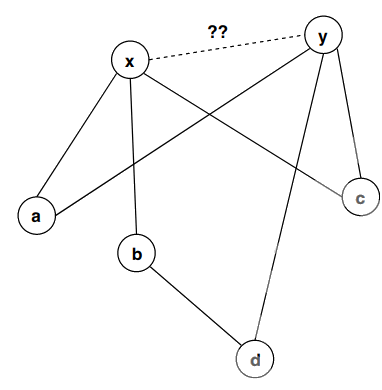
\includegraphics[width=7cm, keepaspectratio]{capitoli/methods/imgs/img6.png}
    \caption{An example illustrating the cycle formation link probability model.}
\end{figure}

Consider a cycle formation model ( \(CF (k)\) ) of degree \((k = 3)\).
The Seed link \((x, y)\), here, can be generated by the following three
mechanisms: - \texttt{random\ link\ occurrence\ g(1)} -
\texttt{length-2\ cycle\ generation\ g(2)}
i.e.~\((x −a −y and x −c −y)\) -
\texttt{length-4\ cycle\ generation\ g(3)} i.e.~\((x −b −d −y)\).

The main issue is to combine several generation mechanisms to compute
total link occurrence probability. The author posits a method to combine
both path and cycle (of different lengths) generation mechanism in the
framework. The expected general clustering coefficient of degree \(k\)
for this model can be estimated as
\[E[C(k)] = f(c_1, c_2, ..., c_k) = \sum_{i} |G_i|p(G_i)p((e_{l, k+1} \in E|G_i)) \]
where \(|G_i|\) is the number of subgraph possible corresponding to the
graph pattern \(G_i\), \(p(G_i)\) is the probability of occurrence of
one of such graphs \(G_i\), and \(p(e_{l,k+l})\) is the probability of
edge \(e_{l,l+1}\) to occur given the pattern \(G_i\). Finally, given
the coefficients, the probability of existence of link is
\[p_{x,y}(c_1, ..., c_k) = \frac{c_1 \prod_{i=2}^{k} c_i^{|path^i_{x,y}|}}{c_1 \prod_{i=2}^{k} c_i^{|path^i_{x,y}|} + (1-c_1)\prod_{i=2}^{k} (1-c_i)^{|path^i_{x,y}|}}\]

\textbf{Liu et al.} proposed degree related clustering coefficient to
quantify the clustering ability of nodes. They applied the same to paths
of shorter lengths and introduced a new index
\texttt{Degree\ related\ Clustering\ ability\ Path\ (DCP)}. They
performed the \texttt{degree\ of\ robustness\ (DR)} test for their index
and showed that missing links have a small effect on the index. Recently
\textbf{Wu et al.} extracted triangle structure information in the form
of node clustering coefficient of common neighbors. Their experiments on
several real datasets show comparable results to the \texttt{CAR} index.
The same concept of the clustering coefficient also introduced in the
work presented by \textbf{Wu et al.}. Authors introduce both node and
link clustering information in their work. Their experiments on
different network datasets showed better performance results against
existing methods, especially on middle and large network datasets.
\textbf{Kumar et al.} explored the concept of node clustering
coefficient to the next level (level-2) that captures more clustering
information of a network. The comprehensive results on several
real-world datasets show better performance compared to local methods
and comparable to the node embedding method \texttt{Node2vec}.
Meanwhile, \textbf{Benson et al.} studied simplicial closure events to
capture higher-order structures in several temporal networks. The
simplicial closure events are the process of closure of timestamped
simplices (simplicial complexes 2 are set of nodes with different sizes)
available in a dataset. These structures are common in several real-time
complex systems, for example, communication in a group, collaboration of
authors for a paper, etc. To assess these higher-order structures, the
authors study the simplicial closure events on triples of nodes (for
simplicity) and suggest that the open triangles or triples of nodes with
strong ties are more likely to close in the future.

\subsection{Structural Perturbation Method}

\textbf{\emph{Lu et al.}} introduced a new framework of computing
predictability of links in the networks. They coined a
\textbf{structural consistency index} to quantify the link
predictability. This index is based on the assumption that ``\emph{links
    in a network are highly predictable if no significant changes occur in
    the structural feature after the addition or deletion of a small
    fraction of the link}''. Based on this index, they proposed a new
similarity index, namely
\texttt{structural\ perturbation\ method\ (SPM)}. The experimental
results show the outstanding performance compared to the
state-of-the-art in their paper.


\tableofcontents

% \chapter{Existing Methods \normalfont{\emoji{bookmark-tabs}}}

Recently, numerous methodologies of link prediction have been
implemented. These methods can be grouped into several categories, like
\textbf{similarity-based, probabilistic models, learning-based models},
etc.

\begin{figure}[H]
    \centering
    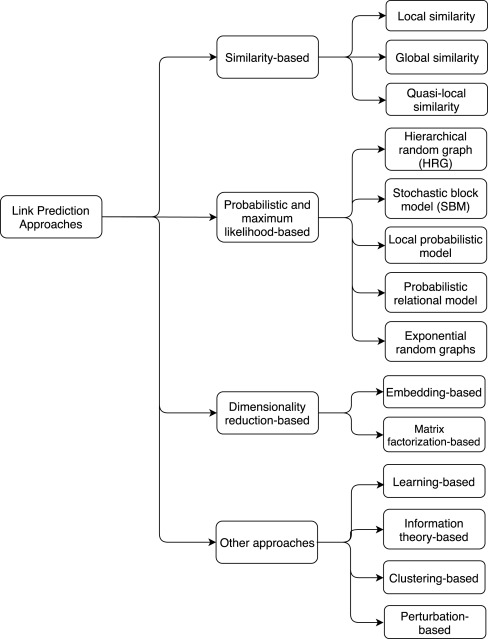
\includegraphics[width=9cm, keepaspectratio]{capitoli/methods/imgs/img2.jpg}
\end{figure}

\section{Similarity-based Methods}

Similarity-based metrics are the simplest one in link prediction, in
which for each pair \(x\) and \(y\), a similarity score \(S(x, y)\) is
calculated. The score \(S(x, y)\) is based on the structural or node's
properties of the considered pair. The non-observed links (i.e.,
\(U - E^T\) ) are assigned scores according to their similarities.
\textbf{The pair of nodes having a higher score represents the predicted
    link between them}. The similarity measures between every pair \emph{can
    be calculated using several properties of the network}, one of which is
structural property. Scores based on this property can be grouped in
several categories like \textbf{local and global}, and so on.

\subsection{Local similarity indices}

Local indices are generally calculated using information about common
neighbors and node degree. These indices \textbf{consider immediate
    neighbors of a node}. The following are some examples of local
similarity indices with a description and method to calculate them:

\begin{itemize}
    \item \texttt{Common\ Neighbors\ (CN)}: In a given network or graph, the size
          of common neighbors for a given pair of nodes \(x\) and \(y\) is
          calculated as the size of the intersection of the two nodes
          neighborhoods ( \(\Gamma\) ). \[S(x, y) = |\Gamma(x) \cap \Gamma(y)|\]
          The likelihood of the existence of a link between x and y increases with
          the number of common neighbors between them.
    \item \texttt{Jaccard\ Coefficient}: This metric is similar to the Common
          Neighbors. Additionally, it normalizes the above score, as given below:
          \[S(x, y) = \frac{|\Gamma(x) \cap \Gamma(y)|}{|\Gamma(x) \cup \Gamma(y)|}\]
          The Jaccard coefficient is defined as the probability of selection of
          common neighbors of pairwise vertices from all the neighbors of either
          vertex. The pairwise Jaccard score increases with the number of common
          neighbors between the two vertices considered. Some researcher
          (\textbf{Liben-Nowell et al.}) demonstrated that this similarity metric
          \textbf{performs worse} as compared to Common Neighbors.
    \item \texttt{Adamic/Adar\ Index\ (AA)}: Adamic and Adar presented a metric to
          calculate a similarity score between two web pages based on shared
          features, which are further used in link prediction after some
          modification
          \[S(x, y) = \sum_{z \in \Gamma(x) \cap \Gamma(y)} \frac{1}{log k_z}\]
          where \(k_z\) is the degree of the node \(z\). It is clear from the
          equation that more weights are assigned to the common neighbors having
          smaller degrees. This is also intuitive in the real-world scenario, for
          example, a person with more number of friends spend less time/resource
          with an individual friend as compared to the less number of friends.
    \item \texttt{Preferential\ Attachment\ (PA)}: The idea of preferential
          attachment is applied to generate a growing scale-free network. The term
          \textbf{growing} represents the incremental nature of nodes over time in
          the network. The likelihood incrementing new connection associated with
          a node \(x\) is proportional to \(k_x\) , the degree of the node.
          Preferential attachment score between two nodes x and y can be computed
          as: \[S(x, y) = k_x k_y\] This index shows the worst performance on most
          networks. The \textbf{simplicity} (as it requires the least information
          for the score calculation) and the \textbf{computational time} of this
          metric are the main advantages. PA shows better results if larger degree
          nodes are densely connected, and lower degree nodes are rarely
          connected. In the above equation, summation can also be used instead of
          multiplication as an aggregate function.
    \item \texttt{Resource\ Allocation\ Index\ (RA)}: Consider two non-adjacent
          vertices \(x\) and \(y\). Suppose node \(x\) sends some resources to
          \(y\) through the common nodes of both \(x\) and \(y\) then the
          similarity between the two vertices is computed in terms of
          \textbf{resources sent} from \(x\) to \(y\). This is expressed
          mathematically as:
          \[S(x, y) = \sum_{z \in \Gamma(x) \cap \Gamma(y)} \frac{1}{k_z}\] The
          difference between \textbf{RA} and \textbf{AA} is that the RA index
          heavily penalizes to higher degree nodes compared to the AA index.
          Prediction results of these indices become almost the same for smaller
          average degree networks. This index shows good performance on
          heterogeneous networks with a high clustering coefficient, especially on
          transportation networks.
    \item \texttt{Cosine\ similarity\ or\ Salton\ Index\ (SI)}: This similarity
          index between two records (documents) is measured by calculating the
          Cosine of the angle between them. The metric is all about the
          orientation and not magnitude. The Cosine similarity can be computed as
          \[S(x, y) = \frac{|\Gamma(x) \cap \Gamma(y)|}{\sqrt{(k_x k_y)}}\] -
          \texttt{Sorensen\ Index}: It is very similar to the Jaccard index.
          \textbf{McCune et al.} show that it \textbf{is more robust than Jaccard
              against the outliers}.
          \[S(x, y) = \frac{2|\Gamma(x) \cap \Gamma(y)|}{k_X + k_y}\]
    \item \texttt{CAR-based\ Common\ Neighbor\ Index\ (CAR)}: CAR-based indices
          are presented based on the assumption that the link existence between
          two nodes is more likely if their common neighbors are members of a
          local community (local-community-paradigm (LCP) theory). In other words,
          the likelihood existence increases with the number of links among the
          common neighbors (local community links (LCLs)) of the seed node pair as
          described in the following figure.
          \[S(x, y) = CN(x, y) \text{ x } LCL(x, y) = CN(x, y) \text{ x } \sum_{z \in \Gamma(x) \cap \Gamma(y)} \frac{|\gamma(z)|}{2} \]
          where \(CN(x, y) = |\Gamma(x) ∩ \Gamma(y)|\) is number of common
          neighbors. \(LCL(x, y)\) refers to the number of local community links
          which are defined as the links among the common neighbors of seed nodes
          x and y. \(\gamma(z)\) is the subset of neighbors of node \(z\) that are
          also common neighbors of \(x\) and \(y\).

          \begin{figure}[H]
              \centering
              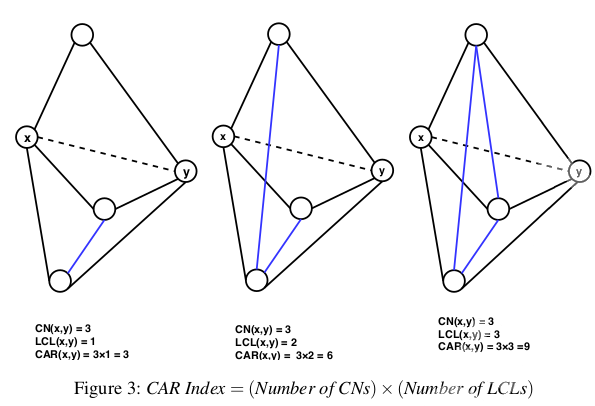
\includegraphics[width=8cm, keepaspectratio]{capitoli/methods/imgs/img3.png}
          \end{figure}
    \item \texttt{CAR-based\ Adamic/Adar\ Index\ (CAA)}: If \(LCL\) is considered
          as an accuracy enhancer, then the \(CAA\) index is obtained by
          incorporating the \(LCL\) theory to the well known AA index and
          mathematically expressed by the equation given below.
          \[S(x, y) = \sum_{z \in \Gamma(x) \cap \Gamma(y)} \frac{|\gamma(z)|}{\log_2(k_z)} \]
    \item \texttt{CAR-based\ Resource\ Allocation\ Index\ (CRA)}: Is a general
          application of the LCL theory to other indices and generate the CRA
          index by incorporating this concept into the existing RA index of the
          literature. Mathematically, the CRA can be expressed as
          \[S(x, y) = \sum_{z \in \Gamma(x) \cap \Gamma(y)} \frac{|\gamma(z)|}{k_z}\]
    \item \texttt{CAR-based\ Preferential\ Attachment\ Index\ (CPA)}: This is
          the preferential attachment index based on the CAR index. CPA is
          obtained by incorporating the LCL theory to the original PA method and
          expressed mathematically by
          \[S(x, y) = e_x e_y + e_x CAR(x, y) + e_y CAR(x, y) + CAR(x, y)^2\]
          where \(e_x\) is the number of neighbors of \(x\) not shared by \(y\)
          and \(CAR(x, y)\) is the similarity score of the node pair \(x\) and
          \(y\) using CAR index. CAR-based methods listed above show the best
          performance on LCP networks. The LCP networks are related to dynamic and
          heterogeneous systems and facilitate network evolution of social and
          biological networks.
    \item \texttt{Hub\ Promoted\ Index\ (HPI)}: This
          similarity index promotes the formation of links between the sparsely
          connected nodes and hubs. It also tries to prevent links formation
          between the hub nodes. This similarity metric can be expressed
          mathematically as
          \[S(x, y) = \frac{|\Gamma(x) \cap \Gamma(y)|}{min(k_x, k_y)}\]
    \item \texttt{Hub\ Depressed\ Index\ (HDI)}: This index is the same as the
          previous one but with the opposite goal as it avoids the formation of
          links between hubs and low degree nodes in the networks. The Hub
          depressed index promotes the links evolution between the hubs as well as
          the low degree nodes. The mathematical expression for this index is
          given below.
          \[S(x, y) = \frac{|\Gamma(x) \cap \Gamma(y)|}{max(k_x, k_y)}\]
    \item \texttt{Local\ Naive\ Bayes-based\ Common\ Neighbors\ (LNBCN)}: The
          above similarity indices are somehow based on common neighbors of the
          node pair where each of the which are equally weighted. This method is
          based on the Naive Bayes theory and arguments that different common
          neighbors play different role in the network and hence contributes
          differently to the score function computed for non-observed node pairs
          \[S(x, y) = \sum_{z \in \Gamma(x) \cap \Gamma(y)} [log(\frac{C(z)}{1 - C(z)}) + log(\frac{1 - \rho}{\rho})]\]
          where \(C(z)\) is node clustering coefficient and \(\rho\) is the
          network density expressed as \[\rho = \frac{|E|}{n(n-1)/2}\]
    \item \texttt{Leicht-Holme-Newman\ Local\ Index\ (LHNL)}: The logic below this
          index is that two vertices are similar to each other if their
          corresponding neighbors are self-similar to themselves. This score is
          defined by the ratio of the path of length two that exits between two
          vertices and the expected path of the same length between them.
          \[S(x, y) = \frac{|\Gamma(x) \cap \Gamma(y)|}{k_x k_y}\]
    \item \texttt{Node\ Clustering\ Coefficient\ (CCLP)}: This index is also based
          on the clustering coefficient property of the network in which the
          clustering coefficients of all the common neighbors of a seed node pair
          are computed and summed to find the final similarity score of the pair.
          Mathematically \[S(x, y) = \sum_{z \in \Gamma(x) \cap \Gamma(y)} C(z)\]
          where \[C(z) = \frac{t(z)}{k_z(k_z - 1)}\] is clustering coefficient of
          the node \(z\) and \(t(z)\) is the total triangles passing through the
          node \(z\).
    \item \texttt{Node\ and\ Link\ Clustering\ coefficient\ (NLC)}:
          This similarity index is based on the basic topological feature of a
          network called ''\emph{Clustering Coefficient}''. The clustering
          coefficients of both nodes and links are incorporated to compute the
          similarity score.
          \[S(x, y) = \sum_{z \in \Gamma(x) \cap \Gamma(y)} \frac{|\Gamma(x) \cap \Gamma(z)|}{k_z -1} \text{ x }C(z) + \frac{|\Gamma(y) \cap \Gamma(z)|}{k_z -1} \text{ x }C(z)\]

\end{itemize}

\subsection{Global similarity indices}

Global indices are computed using entire topological information of a
network. The computational complexities of such methods are higher and
seem to be infeasible for large networks.

\begin{itemize}
    \item \texttt{Katz\ Index}: This
          index can be considered as a variant of the shortest path metric. It
          directly aggregates over all the paths between x and y and dumps
          exponentially for longer paths to penalize them. It can be expressed
          mathematically as:
          \[S(x, y) = \sum_{l = 1}^{\infty}\beta^l|paths_{x, y}^{<l>}| = \sum_{l = 1}^{\infty}\beta^l(A)^l_{x, y}\]
          where, \(paths_{x, y}^{<l>}\) is considered as the set of total \(l\)
          length paths between \(x\) and \(y\), \(\beta\) is a damping factor that
          controls the path weights and A is the adjacency matrix. For the
          convergence of above equation, \[\beta < \frac{1}{\lambda_1} \] where
          \(\lambda_1\) is the maximum eigenvalue of the matrix A. If 1 is added
          to each element of the diagonal of the resulting similarity matrix S,
          this expression can be written in matrix terms as \[S = \beta AS + I\]
          where \(I\) is the identity matrix of the proper dimension. The
          similarity between all pairs of nodes can be directly computed using the
          closed-form by rearranging for \(S\) in the previous expression and
          subtracting the previously added 1 to the elements in the diagonal. Katz
          score for each pair of nodes in the network is calculated by finding the
          similarity matrix as \[S = (I - \beta A)^{- 1} - I\] The computational
          complexity of the given metric is high, and it can be roughly estimated
          to be cubic complexity which is not feasible for a large network.
    \item \texttt{Random\ Walk\ with\ Restart\ (RWR)}: Let \(\alpha\) be a
          probability that a random walker iteratively moves to an arbitrary
          neighbor and returns to the same starting vertex with probability
          \((1 - \alpha)\). Consider \(q_{xy}\) to be the probability that a
          random walker who starts walking from vertex \(x\) and located at the
          vertex \(y\) in steady-state. Now, this probability of walker to reach
          the vertex \(y\) is expressed mathematically as
          \[\overrightarrow{q_x} = \alpha P^T \overrightarrow{q_x} + (1-\alpha) \overrightarrow{e_x}\]
          where \(\overrightarrow{e_x}\) is the seed vector of length \(|V|\)
          (i.e., the total number of vertices in the graph). This vector consists
          of zeros for all components except the elements \(x\) itself. The
          transition matrix \(P\) can be expressed as
          \[\overrightarrow{q_x} = (1-\alpha)(I - \alpha P^T)^{-1} \overrightarrow{e_x}\]
          Since this similarity is not symmetric, the final score between the node
          pair (x, y) can be computed as \[S(x, y) = q_{xy} + q_{yx}\] It is clear
          from the above equation that matrix inversion is required to solve,
          which is quite expensive and prohibitive for large networks.
    \item \texttt{Shortest\ Path}: The inverse relation between the similarity and
          length of the shortest path is captured by the following mathematical
          equation given below. \[S(x, y) = -|d(x, y)|\] where Dijkstra algorithm
          is applied to efficiently compute the shortest path d(x, y) between the
          node pair (x, y). The prediction accuracy of this index is low compared
          to most local indices.
    \item \texttt{Leicht-Holme-Newman\ Global\ Index\ (LHNG)}: This global index
          is based on the principle that two nodes are similar if either of them
          has an immediate neighbor, which is similar to the other node. This is a
          recursive definition of similarity where a termination condition is
          needed. The termination condition is introduced in terms of
          self-similarity, i.e., a node is similar to itself. Thus, the similarity
          score equation consists of two terms: first, the neighbor similarity,
          and the second, self-similarity, as given below.
          \[S(x, y) = \phi  \sum_z A_{x, z} S_{z, y} + \psi \delta_{x, y}\] Here,
          the first term is neighborhood similarity and the second term is
          self-similarity. \(\psi\) and \(\phi\) are free parameters that make a
          balance between these two terms. When the free parameter \(\psi\) = 1,
          this index resembles to the Katz index.
    \item \texttt{Cosine\ based\ on\ L+\ (Cos+)}: Laplacian matrix is extensively
          used as an alternative representation of graphs in spectral graph
          theory. This matrix can be defined as \(L = D - A\), where, \(D\) is the
          diagonal matrix consisting of the degrees of each node of the matrix and
          \(A\) is the adjacency matrix of the graph. The pseudo-inverse of the
          matrix defined by Moore-Penrose is represented as \(L^+\) and each entry
          of this matrix is used to represent the similarity score between the two
          corresponding nodes. The most common way to compute this pseudo-inverse
          is by computing the \textbf{singular value decomposition (SVD)} of the
          Laplacian matrix [$(L = U \Sigma V^{}T)$, where \(U\) and \(V\)
                  are left and right singular vectors of \(SVD\)] as follows
          \[L^+ = V \Sigma^+ U^T\] \(\Sigma^+\) is obtained by taking the inverse
          of each nonzero element of the \(\Sigma\). Further, the similarity
          between two nodes \(x\) and \(y\) can be computed using any inner
          product measure such as Cosine similarity given as
          \[S(x, y) = \frac{L_{x, y}^+}{\sqrt{L_{x, x}^+ L_{y, y}^+}}\]
    \item \texttt{Average\ Commute\ Time\ (ACT)}: This index is based on the
          random walk concept. A random walk is a Markov chain which describes the
          movements of a walker. It defined as the average number of
          movements/steps required by a random walker to reach the destination
          node \(y\), and come back to the starting node \(x\). If \(m(x, y)\) be
          the number of steps required by the walker to reach \(y\) from \(x\),
          then the following expression captures this concept.
          \[n(x, y) = |E| (l_{xx}^+ + l_{yy}^+ - 2l_{xy}^+) \] where \(l_{xy}^+\)
          denotes the \((x, y)\) entry of the matrix \(L^+\) . Pseudo-inverse of
          the Laplacian, \(L^+\) can be computed as
          \[L^+ = (L - \frac{ee^T}{n})^{-1} + \frac{ee^T}{n}\] where \(e\) is a
          column vector consisting of 1's. Smaller value of this equation will
          represent higher similarity. The final expression is the following
          \[S(x, y) = \frac{1}{l_{xx}^+ + l_{yy}^+ - 2l_{xy}^+}\]
    \item \texttt{Normalized\ Average\ Commute\ Time\ (NACT)}: This is a variant
          of ACT that takes into account node degrees. For a high degree node
          (hub) \(y\), \(m(x, y)\) is usually small regardless of \(x\), the
          similarity measure is normalized with stationary distribution \(\pi\) of
          the Markov chain describing random walker on the graph. This normalized
          measure can be computed with the following equation
          \[S(x, y) = \frac{1}{(m(x, y)\pi_y + m(y, x)\pi_x)}\]
    \item \texttt{Matrix\ Forest\ Index\ (MF)}: his index is based on the concept
          of spanning tree which is defined as the subgraph that spans total nodes
          without forming any cycle. The spanning tree may contain total or less
          number of links as compared to the original graph. Chebotarev and Shamis
          proposed a theorem called matrix-forest theorem which states that the
          number of spanning tree in a graph is equal to the co-factor of any
          entry of Laplacian matrix of the graph. Here, the term forest represents
          the union of all rooted disjoint spanning trees. The similarity between
          two nodes \(x\) and \(y\) can be computed with the equation given below
          \[S = (I + L)^{-1}\] where \((I + L)\_{(x,y)}\) is the number of
          spanning rooted forests ( \(x\) as root ) consisting of both the nodes
          \(x\) and \(y\). Moreover, this quantity is equal to the co-factor of
          \((I + L)_{(x,y)}\) .
    \item \texttt{SimRank}: This is a measure of
          structural context similarity and shows object-to-object relationships.
          It is not domain-specific and recommends to apply in directed or mixed
          networks. The basic assumption of this measure is that two objects are
          similar if they are related to similar objects. SimRank computes how
          soon two random walkers meet each other, starting from two different
          positions. This measure can be represented in matrix form as
          \[S(x,y) = \alpha W^T SW + (1 - \alpha)I\] where, \(\alpha \in (0, 1)\)
          is a constant. \(W\) is the transformation matrix and computed by
          normalizing each column of adjacency matrix \(A\) as
          \[
              W_{ij} = \frac{a_{ij}}{\sum_{k=1}^{n}}
          \]
          The computational complexity
          of this measure is high for a large network, and to reduce its time, the
          authors suggest pruning recursive branches.
    \item \texttt{Rooted\ Pagerank\ (RPR)}: The idea of PageRank was originally
          proposed to rank the web pages based on the importance of those pages.
          The algorithm is based on the assumption that a random walker randomly
          goes to a web page with probability \(\alpha\) and follows hyper-link
          embedded in the page with probability \((1 - \alpha)\). Chung et
          al.~used this concept incorporated with a random walk in link prediction
          framework. The importance of web pages, in a random walk, can be
          replaced by stationary distribution. The similarity between two vertices
          \(x\) and \(y\) can be measured by the stationary probability of \(y\)
          from \(x\) in a random walk where the walker moves to an arbitrary
          neighboring vertex with probability \(\alpha\) and returns to \(x\) with
          probability \((1 - \alpha)\). Mathematically, this score can be computed
          for all pair of vertices as
          \[RPR = (1 - \alpha)(I - \alpha \hat{N})^{-1}\] where
          \(\hat{N} = D^{-1} A\) is the normalized adjacency matrix with the
          diagonal degree matrix \(D[i, i] = \sum_j A[i, j]\).
\end{itemize}

\subsection{Quasi-local indices}

Quasi-local indices have been introduced as a trade-off between local
and global approaches or performance and complexity. These metrics are
as efficient to compute as local indices. Some of these indices extract
the entire topological information of the network. The time complexities
of these indices are still below compared to the global approaches.

\begin{itemize}
    \item \texttt{Local\ Path\ Index\ (LP)}: This metric has the intent to furnish
          a good trade-off between accuracy and computational complexity. The
          metric is expressed mathematically as \[S^{LP} = A^2 + \epsilon A^3\]
          where $\epsilon$ represents a free parameter. Clearly, the measurement
          converges to common neighbor when \(\epsilon = 0\). If there is no
          direct connection between \(x\) and \(y\), \((A^3)_{xy}\) is equated to
          the total different paths of length 3 between \(x\) and \(y\). The index
          can also be expanded to generalized form
          \[S^{LP} = A^2 + \epsilon A^3 + \epsilon^2 A^4 + ... + \epsilon^{(n−2)} A^n\]
          where \(n\) is the maximal order. Computing this index becomes more
          complicated with the increasing value of \(n\). The LP index outperforms
          the proximity-based indices, such as RA, AA, and CN.
    \item \texttt{Path\ of\ Length\ 3\ (L3)}: Georg Simmel, a German sociologist,
          first coined the concept ``triadic closure'' and made popular by Mark
          Granovetter in his work ``\emph{The Strength of Weak Ties}''. The
          authors proposed a similarity index in protein-protein interaction (PPI)
          network, called \textbf{\emph{path of length 3 (or L3)}} published in
          the Nature Communication. They experimentally show that the triadic
          closure principle (TCP) does not work well with PPI networks. They
          showed the paradoxical behavior of the TCP (i.e., the path of length 2),
          which does not follow the structural and evolutionary mechanism that
          governs protein interaction. The TCP predicts well to the interaction of
          self-interaction proteins (SIPs), which are very small (4\%) in PPI
          networks and fails in prediction between SIP and non SIP that amounts to
          96\%. They showed that the L3 index performs well in such conditions and
          give mathematical expression to compute this index as
          \[S(x, y) = \sum \frac{a_{x,u} a_{u,v} a_{v,y}}{k_u k_v}\]
    \item \texttt{Similarity\ based\ on\ Local\ Random\ Walk\ and\ Superposed\ Random\ Walk\ (LRW\ and\ SRW)}:
          This metric propose a new similarity measures by exploiting the random
          walk concept on graphs with limited walk steps. They defined node
          similarity based on random walks of lower computational complexity
          compared to the other random walk based methods. Given a random walker,
          starting from the node \(x\), the probability of reaching the random
          walker to the node \(y\) in \(t\) steps is
          \[\overrightarrow{\pi}\_x(t) = P^T \overrightarrow{\pi}\_x(t-1)\] where
          \(\overrightarrow{\pi}\_x(0)\) is a column vector with \(x^{th}\)
          element as 1 while others are 0's and \(P^T\) is the transpose of the
          transition probability matrix \(P\). \(P_{xy}\) entry of this matrix
          defines the probability of a random walker at node \(x\) will move to
          the next node \(y\). It is expressed as \(P_{xy} = \frac{a_{kx}}{k_x}\)
          , where \(a_{xy}\) is 1 when there is a link between \(x\) and \(y\) and
          0, otherwise. The authors computed the similarity score ( \(LRW\) )
          between two nodes based on the above concept as
          \[S^{LRW}(x, y) = \frac{k_x}{2|E|}\pi_{xy}(t) + \frac{k_y}{2|E|}\pi_{xy}(t)\]
          This similarity measure focus on only few steps covered by the random
          walker (hence quasi-local) and not the stationary state compared to
          other approaches. Random walk based methods suffer from the situation
          where a random walker moves far away with a certain probability from the
          target node whether the target node is closer or not. This is an obvious
          problem in social networks that show a high clustering index i.e.,
          clustering property of the social networks. This degrades the similarity
          score between the two nodes and results in low prediction accuracy. One
          way to counter this problem is that continuously release the walkers at
          the starting point, which results in a higher similarity between the
          target node and the nearby nodes. By superposing the contribution of
          each walker (walkers move independently), SRW is expressed as
          \[S^{SRW} (x, y) (t) = \sum_{l=1}^{t} S^{LRW} (l)\]
\end{itemize}

\subsection{Some Remarks}

Similarity-based approaches mostly focus on the structural properties of
the networks to compute the similarity score. \textbf{\emph{Local
        approaches}} consider, in general, neighborhood information (direct
neighbors or neighbors of neighbor), which take less time for
computation. This is the property that makes the local approaches
feasible for massive real-world network datasets. \textbf{\emph{Global
        approaches}} consider the entire structural information of the network;
that is why time required to capture this information is more than local
and quasi-local approaches. Also, sometimes, entire topological
information may not be available at the time of computation, especially
in a decentralized environment. So, parallelization over the global
approaches may not possible or very complex compared to the local and
quasi-local approaches. The performance or prediction accuracy of these
approaches (i.e., global approaches) is better compared to local and
quasi-local. \textbf{\emph{Quasi-local approaches}} extract more
structural information than local and somehow less information compared
to the global.


\section{Probabilistic and maximum likelihood models}

For a given network \(G(V, E)\), \textbf{\emph{the probabilistic model
        optimizes an objective function to set up a model that is composed of
        several parameters}}. Observed data of the given network can be
estimated by this model nicely. At that point, the likelihood of the
presence of a non-existing link \((i, j)\) is evaluated using
conditional probability \(P(A_{i j} = 1 | \Theta )\). Several
\texttt{probabilistic\ models} and \texttt{maximum\ likelihood\ models}
have been proposed in the literature to \textbf{infer missing links in
    the networks}.\\

\textbf{The probabilistic models normally require more information like
    node or edge attribute knowledge in addition to structural information}
Extracting these attribute information is not easy; moreover, the
parameter tuning is also a big deal in such models that limit their
applicability. \emph{Maximum likelihood methods are complex and
    time-consuming}, so these models are not suitable for real large
networks.

\subsection{Local probabilistic model for link prediction}

\textbf{Wang et al.} proposed a \texttt{local\ probabilistic\ model} for
link prediction in an \emph{undirected network}. They employed three
different types of features viz., topological, semantic, and
cooccurrence probability features extracted from different sources of
information.\\

They presented an idea of a central neighborhood set derived from the
local topology of the considered node-pair, which is relevant
information for the estimation of a link between them. They computed
non-derivable frequent itemsets (i.e., those itemsets whose occurrence
statistics can not be derived from other itemset patterns) from the
network events log data, which is further used as training data for the
model. An event corresponds to a publication of a paper (i.e., authors'
interactions in the paper is a an event, and a set of such events is the
event log) in the Coauthorship network. The model is shown in the
following Figure, which considers the approach described below.\\

First, the central neighborhood set between \(x\) and \(y\) is
calculated based on local event log data. One of the usual ways to find
the central neighborhood set is to find the \textbf{shortest path
    between two vertices of specified length}, and the vertices are lying on
this path can be included in the required set. There can be more than
one shortest path between two vertices, so more neighborhood sets can be
possible. Neighborhood sets of shorter lengths and more frequent
(frequency score is used when more shortest paths of the same length are
available) are chosen for the central neighborhood set. The authors
considered the shortest path up to length 4 since the nodes lying on the
shorter length path are more relevant.\\

In the second step, for a given central neighborhood set, non-derivable
frequent itemsets are used to learn the local probabilistic model.
\textbf{Calders et al.} proposed a depth-first search method to
calculate non-derivable itemsets and the same algorithm used by the
authors. Why non-derivable frequent itemsets? \textbf{Pavlov et al.}
first introduced the concept of frequent itemset to construct an
\texttt{MRF}. They argued that a \(K-itemset\) and its support
represents a \(K-way\) statistics, which can be viewed as a constraint
on the true underlying distribution that generates the data. Given a set
of itemset constraints, a maximum entropy distribution satisfying all
these constraints is selected as the estimate for the true underlying
distribution. This maximum entropy distribution is equivalent to an
\texttt{MRF}. Since the number formed links are very few compared to all
possible links in a sparse network, the authors used a support threshold
of one to extract all frequent itemsets. Theses extracted itemsets are
large in number that results in expensive learning for the \texttt{MRF}.
To reduce this cost, only non-derivable itemsets are extracted. They
find all such itemsets that lie entirely within the central neighborhood
set. Using these itemsets, a \texttt{Markov\ Random\ Field} is
\textbf{learned}.\\

In the last step, the \texttt{iterative\ scaling\ algorithm} is used to
learn a local \texttt{MRF} for the given central neighborhood set. This
process continues overall itemset constraints and continuously updates
the model until the model converges. Once the model learning process is
over, one can infer the co-occurrence probability by computing the
marginal probability over the constructed model. The
\texttt{Junction\ tree\ inference\ algorithm} is used to infer
co-occurrence probability. The algorithm to induce co-occurrence
probability feature for a pair of vertices can be found in
\href{https://static.aminer.org/pdf/PDF/000/303/209a_parameterized_probabilistic_model_of_network_evolution_for_supervised_link.pdf}{Local
    Probabilistic Models for Link Prediction}.

\subsection{Probabilistic relational model for link prediction (PRM)}

Existing works show that \textbf{node attributes play a significant role
    to improve the link prediction accuracy}. However, \textbf{no generic
    framework is available to incorporate node and link attributes} and
hence, not applicable to all scenarios. To this end, \textbf{the
    probabilistic model is a good and concrete solution that provides a
    systematic approach to incorporate both node and link attributes in the
    link prediction framework}. Pioneering works on \texttt{PRM} include
\textbf{Getoor et al.} study on directed networks, \textbf{Taskar et
    al.} study on undirected networks, \textbf{Jennifer Neville}
work on for both networks, etc. published in \texttt{JMLR} is based on
\texttt{Relational\ Bayesian\ network\ (RBN)} where relation links are
directed and published in NIPS is based on
\texttt{Relational\ Markov\ network\ (RMN)} where relational links are
undirected.\\

\texttt{PRM} was originally designed for attribute prediction in
relational data, and it later extended to link prediction task. The
authors employed the attribute prediction framework to link prediction.
This casting can be understood with the following example: - Consider
the problem of link prediction in a coauthorship network. Non-relational
frameworks of link prediction consider only one entity type
``\emph{person}'' as node and one relationship; however, relational
framework (\texttt{PRMs}) include more entity types like article,
conference venue, institution, etc. Each entity can have attributes like
a person (attributes: name, affiliation institute, status (student,
professor)), article (attributes: publication year, type (regular,
review)), etc. Several relational links may possible among these
entities like advisor-advisee/research scholar relation between two
persons, author relationship between person and paper entities, and
paper can be related to the conference venue with publish relationship.
Moreover, relationships (links) among these entities can also have
attributes viz., exists (if there is a link between the two involved
entities), or not-exist (no link between the involved entities). This
way, the link prediction can be reduced to an attribute prediction
framework/model.\\

During the model training, a single link graph is constructed that
incorporates above heterogeneous entities and relationships among them.
Model parameters are estimated discriminatively to maximize the
probability of the link existence and other parameters with the given
graph attribute information. The learned model is then applied using
probabilistic inference to predict missing links.\\

\subsection{Hierarchical structure model (HSM)}

These models are based on the assumption that the structures of many
real networks are hierarchically organized, where nodes are divided into
groups, which are further subdivided into subgroups and so forth over
multiple scales. Some representative work systematically encodes such
structures from network data to build a model that estimates model
parameters using statistical methods. These parameters are then used in
estimating the link formation probability of unobserved links.\\

Some studies suggest that many real networks, like biochemical networks
(protein interaction networks, metabolic networks, or genetic regulatory
networks), Internet domains, etc. are hierarchically structured. In
hierarchical networks, vertices are divided into groups, which are
further sub-divided into subgroups and so forth over multiple scales.
\textbf{Clauset et al.} proposed a probabilistic model that takes a
hierarchical structure of the network into account. The model infers
hierarchical information from the network data and further applies it to
predict missing links.\\

The hierarchical structures are represented using a tree (binary), or
dendrogram, where, the leaves (i.e., \(n\) ) represent the number of
total vertices in the network and each internal vertex out of (
\(n - 1\) ) corresponds to the group of vertices descended from it. Each
internal vertex \(r\) is associated with a probability \(p_r\) , then
the existing edge probability \(p_{xy}\) between two vertices \(x\) and
\(y\) is given by \(p_{xy} = p_r\) where, \(r\) is their lowest common
ancestor. The hierarchical random graph is then, represented by the
dendrogram \(D^{\star}\) with the set of probability \(\{ p_r \}\) as
\(\left( D^{\star},\{p_r\} \right)\). Now the learning task is to find
the hierarchical random graph(s) that best estimates the observed
real-world network data. Assuming all possible dendrograms to be equally
likely, Bayes theorem says that the probability of the dendrogram
\(\left(D^{\star}, \{p_r\} \right)\) that best estimates the data is
proportional to the posterior probability or likelihood, \(L\) from
which the model generates the observed network and our goal is to
maximize \(L\) . The likelihood of a hierarchical random graph
\(\left(D^{\star},\{p_r\} \right)\) is computed using the following
equation

\[
    L(D^{\star}, \{p_r\}) = \prod_{r \in D^{\star}} p_r^{E_r} (1-p_r)^{L_r R_r - Er},
\]

where \(L_r\) and \(R_r\) are the left and right subtree rooted at
\(r\), and \(E_r\) is the number of links in the network whose endpoints
have \(r\) as their lowest common ancestor in \(D^{\star}\) . The above
equation assumes the convention \(0^0 = 1\). For a given dendrogram
\(D^{\star}\) , it is easy to compute the probability \(p_r\) that
maximizes \(L(D^{\star}, \{p_r\})\) i.e.

\[
    \overline{p_r} = \frac{E_r}{L_r R_r}.
\]

This can be understood with the following example illustrated in the
next Figure. Now, this model can be used to estimate the missing links
of the network as follows. Sample a large number of dendrograms with
probability proportional to their likelihood. Then, compute the mean
connecting probability \(\overline{p_{xy}}\) of each nonexisting pair
\((x, y)\) by averaging the corresponding probability \(p_{xy}\) overall
sampled dendrograms. Sort these vertices pairs scores in descending
order and selects top-l links to be predicted.

\begin{figure}[H]
    \centering
    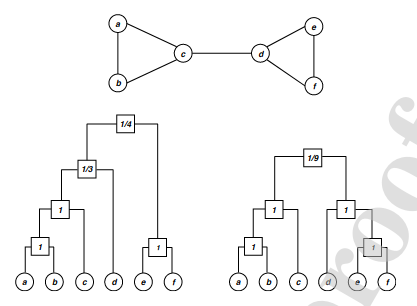
\includegraphics[width=8cm, keepaspectratio]{capitoli/methods/imgs/img8.png}
    \caption{ An illustrating example of \texttt{HSM} for a graph of 6 nodes and its
        two possible dendrograms. The internal nodes of each dendrogram are
        labeled as the maximum likelihood probability \(\overline{p}_r\). The
        likelihoods of the left and the right dendrograms are
        \(L(D1) = (1/3)(2/3)^2 (1/4)^2(3/4)^6\) \(= 0.00165\), and
        \(L(D2) = (1/9)(8/9)^8 = 0.0433\). Thus, the second (i.e., right)
        dendrogram is most probable as it divides the network in a balanced one
        at the first level.}
\end{figure}

\subsection{Stochastic block model (SMB)}

Hierarchical structures may not represent most networks. A more general
approach to represent these networks is block model where vertices are
distributed (partitioned) into blocks or communities and the connecting
probability between two vertices depends on blocks they belong to.
\textbf{Guimera et al.} presented a novel framework where stochastic
block model representation of a network is employed to find missing and
spurious links. The authors compute the reliability of the existence of
links given an observed network that is further used to find missing
links (non-existing links with higher reliabilities) and spurious links
(existing links with lower probabilities).\\

The link reliability \(R_{xy}\) between the two vertices \(x\) and \(y\)
is

\[R_{xy} = p_{BM} (A_{xy} = 1 | A^0).\]

i.e.~probability that the link truly exists given the observed network
\(A^0\), the block model \(BM\).\\

Generally, complex networks are outcomes of combination of mechanisms,
including modularity, role structure, and other factors. In \(SBM\),
partitioning vertices of network based on these mechanisms may result in
different block models that capture different correlations (patterns) of
the network. Assume that no prior knowledge of suitable models, the
reliability is expressed as

\[
    R_{xy} = \frac{1}{Z} \sum_{P \in P^{\star}} \left( \frac{l^{0}_{\sigma_x \sigma_y} + 1}{r^{0}_{\sigma_x \sigma_y + 2}} \right) \text{ exp } \left[ -H(P) \right],
\]

where the sum is over all possible partitions \(P^{\star}\) of the
network into groups, \(\sigma_x\) and \(\sigma_y\) are vertices \(x\)
and \(y\) groups in partition \(P\) respectively. Moreover, \(l^0_1\)
and \(r^0_{\sigma_{\alpha} \sigma_{\beta}}\) are the number of links and
maximum possible links in the observed network between groups \(\alpha\)
and \(\beta\) . The function \(H(P)\) is

\[H(P) = \sum_{\alpha \leq \beta} \left[ \ln \left( r_{\alpha \beta} \right) + \ln \binom {r_{\alpha \beta}}{l^0_{\alpha \beta}} \right],\]

and \(Z = \sum_{P \in P^{\star}} \text{ exp } \left[ -H(P) \right]\).\\

Practically, solving equation \(R_{xy} = \ldots\) , i.e., summing over
all possible partitions is too complex even for a small network.
However, the Metropolis algorithm can be used to correctly sample the
relevant partitions and obtain link reliability estimates.\\

The authors employed the link reliability concept to find missing links
and to identify the spurious link in the networks with the following
procedure.

\begin{itemize}
    \item
          \((i)\) Generate the observed network \(A^0\) by removing/adding some
          random links (for finding missing/spurious links) from/to the true
          network \(A^t\) .
    \item
          \((ii)\) Compute the link reliability for non-observed links (i.e.
          non-existing \(+\) missing/spurious links).
    \item
          \((iii)\) Arrange these links with their reliability score in
          decreasing order and decide the top-l links as desired ones (i.e.,
          missing/spurious links).
\end{itemize}

Probabilistic and maximum likelihood methods extract useful features and
valuable correlation among the data using hierarchical and stochastic
block models, which result in significant improvements in prediction
results as compared to some similarity-based methods. However, these are
\textbf{quite complex and time-consuming even on small datasets} that
limit their applicability on large scale real-world network datasets.

\subsection{Exponential random graph model (ERGM) or P-star model}

\section{Link prediction using Dimensionality Reduction}

The curse of dimensionality is a well-known problem in machine learning.
Some researchers employ dimension reduction techniques to tackle the
above problem and apply it in the \textbf{link prediction} scenario.

\subsection{Embedding-based link prediction}

The network embedding is considered as a dimensionality reduction
technique in which higher \(D\) dimensional nodes (vertices) in the
graphs are mapped to a lower \(d\) (\(d << D\)) \textbf{dimensional
    representation (embedding)} space by preserving the node neighborhood
structures. In other words, \textbf{\emph{find the embedding of nodes to
        a lower d-dimensions such that similar nodes (in the original network)
        have similar embedding (in the representation space)}}.\\ In the Figure
below you can see an application example of a dimensionality reduction
technique to a graph that represent a social network.

\begin{figure}[H]
    \centering
    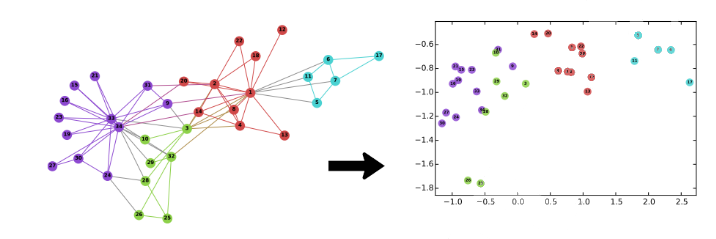
\includegraphics[width=12cm, keepaspectratio]{capitoli/methods/imgs/img4.png}
\end{figure}

The main component of the network embedding is the encoding function or
encoder \(f_{en}\) that map each node to the embedding space
\[f_{en}(x) = z_x\] where \(z_x\) is the \(d\)-dimensional embedding of
the node \(x\). The embedding matrix is \(Z \in R^{d x |V|}\), each
column of which represents an embedding vector of a node.\\

\begin{figure}[H]
    \centering
    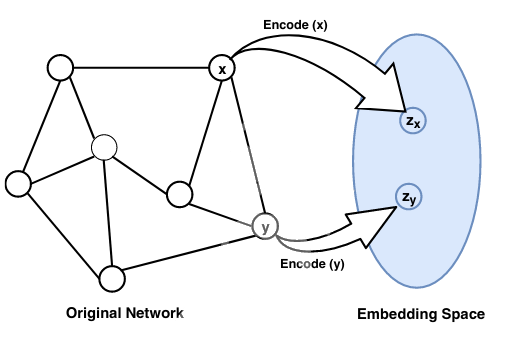
\includegraphics[width=10cm, keepaspectratio]{capitoli/methods/imgs/img5.png}
\end{figure}

Now, a similarity function is \(S(x, y)\) is defined that specifies how
to model the vector (embedding) space relationships equivalent to the
relationships in the original network, i.e.,
\[S(x, y) \approx z_x^T z_y\]

Here \(S(x, y)\) is the function that reconstructs pairwise similarity
values from the generated embedding. The term \(S(x, y)\) is the one
that differ according to the function used in different
factorization-based embedding approaches.\\

For example, \texttt{graph\ factorization} directly employ adjacency
matrix \(A\) i.e.~\((S(x, y) \overset{\Delta}{=} A_{(x,y)})\) to capture
first order proximity, \texttt{GraRep} selects
\((S(x, y) \overset{\Delta}{=} A^2_{(x,y)})\) and \texttt{HOPE} uses
other similarity measures(e.g. Jaccard neighborhood overlap). Most
embedding methods realize the reconstruction objective by minimizing the
loss function, L
\[L = \sum_{(x, y) \in \{V x V \}} l(z_x^T z_y, S(x, y))\]

Once the previous equation is \textbf{converged}
(i.e.~\textbf{trained}), one can use the trained encoder to generate
nodes embedding, which can further be employed to infer missing link and
other downstream machine learning tasks.\\

Recently, some network embedding techniques have been proposed and
applied successfully in link prediction problem. The
\texttt{Laplacian\ eigenmaps},
\texttt{Logically\ linear\ embedding\ (LLE)}, and \texttt{Isomap} are
examples based on the simple notion of embedding. Such embedding
techniques are having quite complex in nature and face scalability
issues. To tackle the scalability issue, graph embedding techniques have
leveraged the sparsity of real-world networks. For example,
\texttt{DeepWalk} extracts local information of truncated random walk
and embeds the nodes in representation space by considering the walk as
a sentence in the language model. It preserves higher order proximity by
maximizing the probability of co-occurrence of random walk of length
\(2k + 1\) (previous and next \(k\) nodes centered at a given node).
\texttt{Node2vec} also uses a random walk to preserves higher order
proximity but it is biased which is a trade-off between the
\texttt{breadth-first\ search\ (BFS)} and
\texttt{depth-first\ search\ (DFS)}.\\

The experimental results show that the \texttt{Node2vec} performs better
than the \texttt{Deepwalk}.\\

In next step, \textbf{Trouillon et al.} introduced complex embedding in
which simple matrix and tensor factorization have been used for link
prediction that uses a vector with complex values. Such composition of
complex embedding includes all possible binary relations especially
symmetric and anti-symmetric relations. Recently, some more studies have
been published in link prediction using embedding, for example,
\textbf{Cao et al.~subgraph embedding}, \textbf{Li et al.~deep dynamic
    network embedding}, \textbf{Kazemi et al.}, etc.

\subsection{Matrix factorization/decomposition-based link prediction}

From last decade, matrix factorization has been used in lots of papers
based on link prediction and recommendation systems. Typically, the
latent features are extracted and using these features, each vertex is
represented in latent space, and such representations are used in a
supervised or unsupervised framework for link prediction. To further
\textbf{improve the prediction results, some additional node/link or
    other attribute information can be used}. In most of the works,
non-negative matrix factorization has been used. Some authors also
applied the singular value decomposition technique. Let the input data
matrix is represented by \(X = (x_1, x_2, ..., x_n)\) that contains
\(n\) data vectors as columns. Now, factorization of this matrix can be
expressed as \[X \approx FG^T\] where
\(X \in R^{p x n}, F \in R^{p x k} , and G \in R^{n x k}\) . Here, \(F\)
contains the bases of the latent space and is called the basis matrix.
\(G\) contains combination of coefficients of the bases for
reconstructing the matrix \(X\) , and is called the coefficient matrix.
\(k\) is the dimension of latent space \((k < n)\). Several well-known
matrix factorizations are expressed based on some constraints on either
of the three matrices, for example

\begin{itemize}
    \item \texttt{SVD}:
          \(X_\pm \approx F_\pm G_\pm^T\)
    \item \texttt{NMF}:
          \(X_+ \approx F_+ G_+^T\)
    \item \texttt{Semi-NMF}:
          $X_\pm \approx F_\pm G_+\^{T} $
    \item \texttt{Convex-NMF}:
          $X_\pm \approx  X_\pm W_+ G_\pm^{T}$
\end{itemize}

In the above four equations, \(Z_\pm\) represents the nature of the
entries in the matrix \(Z\), i.e.~both positive and negative entries
allowed in the matrix \(Z\). In the last equation, \(F = XW\) represents
the convex combinations of the columns of \(F\) . Generally, such a
factorization problem can be modeled as the following
\texttt{Frobenius\ norm\ optimization\ problem}
\[min_{f, g} ||X - FG^T||^2_{fro}\]
\[\text{subject to} F \ge 0, G \ge 0\] Here \(||Z||^2_{fro}\) is the
frobenius norm of \(Z\) and the constraints represent NMF factorization.
However, any of the above four constraints can be used depending on the
requirement of the problem underlying. After solving the above
optimization problem, the similarity between a non-existing pair
\((x, y)\) can be computed by the similarity of the \(x^{th}\) and
\(y^{th}\) row vectors in the coefficient matrix \(G\).

\begin{itemize}
    % \tightlist
    \item
          \texttt{Acar\ et\ al.} expressed temporal link prediction as a matrix
          completion problem and solve it through the
          \texttt{matrix\ and\ tensor\ factorization}. They proposed a weighted
          method to collapsed the temporal data in a single matrix and factorize
          it using \texttt{CANDECOMP/PARAFAC\ (CP)} tensor decomposition method.
    \item
          \texttt{Ma\ et\ al.} also applied matrix factorization to temporal
          networks where features of each network are extracted using
          \texttt{graph\ communicability} and then collapsed into a single
          feature matrix using \texttt{weighted\ collapsing\ tensor\ (WCT)}.
          They showed the equivalence between eigen decomposition of
          \texttt{Katz\ matrix} and
          \texttt{non-negative\ matrix\ factorization\ (NMF)} of the
          communicability matrix that serves as the foundation of their
          framework.
    \item
          \texttt{Menon\ et\ al.} proposed a work for structural link
          prediction. Here, the problem is modeled as
          \texttt{matrix\ completion\ problem}, and
          \texttt{matrix\ factorization} are used to solve it. They introduced a
          supervised matrix decomposition framework that learns latent
          (unobserved) structural features of the graph and incorporates it with
          additional node/link explicit feature information to make a better
          prediction. Additionally, they allowed the factorization model to
          solve class imbalance problem by optimizing ranking loss.
    \item
          \texttt{Chen\ et\ al.} proposed a work, where the authors extracted
          topological matrix and attribute matrix and factorized these matrices
          using \texttt{non-negative\ matrix\ factorization}. The final score
          matrix is obtained by integrating these two matrices in the latent
          space.
\end{itemize}
\section{Other approaches}

\subsection{Learning-based frameworks for link prediction}

Earlier described approaches (e.g., similarity and probabilistic
methods) deal with the computing a score of each non-observed link
either by a similarity or a probabilistic function. However, \textbf{the
    link prediction problem can also be modeled as a learning-based model}
to exploit graph topological features and attribute information. The
problem is cast as a \textbf{supervised classification model} where a
\textbf{point} (i.e., training data) \textbf{corresponds to a
    vertex-pair in the network}, and the \textbf{label} of the point
\textbf{represents the presence or absence of an edge (link) between the
    pair}.\\ In other words, \emph{consider a vertex-pair} \(\mathit{(x, y)}\)
\emph{in the graph} \(\mathit{G(V, E)}\) \emph{and the label of the
    corresponding data point in the classification model is}
\(\mathit{l_{(x,y)}}\) . Then,

\[l_{(x, y)}=
    \begin{cases}
        +1 \ \text{ if } (x, y) \in E \\
        -1 \ \text{ if } (x, y) \notin E
    \end{cases}
\]

\textbf{This is typically a binary classification task} where several
classifiers (e.g.,
\texttt{decision\ tree,\ naive\ Bayes,\ support\ vector\ machine}, etc.)
can be employed to predict the label of unknown data points
(corresponding to missing links in the network). One of the major
challenges of this model (i.e., machine learning) is the
\textbf{selection of appropriate feature set}. Majority of the existing
research works extract feature sets from the network topology (i.e.,
topological information of the network). These \textbf{features are
    generic} and domain-independent that are \textbf{applicable to any
    network}. Such features are typical,
\texttt{neighborhood,\ and\ path-based\ features}.\\ Some other works
concentrate on extracting node and edge features that play a crucial
role to improve the performance of link prediction. The cost of
extraction of such features is cheap and easy, while the main
disadvantage is the domain-specific nature of them.

\subsection{Information theory-based link prediction}

Several complex networks have utilized the concept of
\textbf{information theory to compute their complexity on different
    scales}. They defined several correlation measures and modeled some
networks (e.g., \texttt{star,\ tree,\ lattice,\ ER\ graph}, etc.).
\textbf{Bauer et al.} used the \texttt{maximum\ entropy\ principle} to
assign a statistical weight to any graph and introduced random graph
construction with arbitrary degree distribution.\\

\textbf{Tan et al.} posed the link prediction problem in the
\texttt{framework\ of\ information\ theory}. They mainly focus on local
assortativity to capture local structural properties of the network and
showed that \texttt{mutual\ information\ (MI)} method performs well on
both low and highly correlated networks. Motivated by, \textbf{Zhu, B.
    and Xia} added more local features (i.e., links information of neighbors
of the seed nodes as well as their common neighbors) in their framework
and called it as \texttt{neighbor\ set\ information\ (NSI)\ index}.
Thus, they showed that the different features could be combined in an
information-theoretic model to improve the link prediction accuracy.\\

\textbf{Xu et al.} considered path entropy as a similarity metric for
the link prediction problem. The authors assumed that there is no
correlation among the degrees of the nodes in the network. Consider the
following notations based on their paper: \(L^0_{xy}\) shows no link
exists between two vertices \(x\) and \(y\), and the corresponding
existence is represented by \(L^1_{xy}\). Probability of existence of a
link between the above two vertices is given as

\[
    P(L^1_{xy}) = 1 - P(L^0_{xy}) = 1 - \frac{C^{k_y}_{M-k_x}}{C^{k_y}_M}
\]

where \(C_M^{k_Y}\) represents the number of candidate link sets for the
vertex \(y\) with all links incident with \(y\) and \(C^{k_y}_{M-k_x}\)
denotes the number of candidate link sets for the vertex \(y\) with all
links incident with \(y\) but none of them is incident with \(x\).
Outcome results on several networks demonstrate that the similarity
index based on path entropy performs better than other indices in terms
of prediction accuracy and precision. \textbf{Xu et al.} extend the
previous work to the weighted network by considering the weight of the
paths. Recently, some more efforts have been applied in this direction
based on different features of the networks like influential nodes,
combining node attributes with
\texttt{structural\ similarity,\ local\ likelihood,\ and\ maximal\ entropy\ random\ walk}.

\subsection{Clustering-based Link Prediction}

\textbf{Huang} presented a paper on
\texttt{graph\ topology-based\ link\ prediction} where a
\texttt{generalized\ clustering\ coefficient} is used as a
\textbf{predictive parameter}. The author introduces a \textbf{cycle
    formation model} that shows the relationship between link occurrence
probability and its ability to form different length cycles. This model
suggests that the occurrence probability of a particular link depends on
the number of different lengths cycles formed by adding this link. The
model is based on the assumption of the stationary property of the
degree of clustering of the network. This model captures longer cycles
by extending the higher-order clustering coefficients and defines the
generalized clustering coefficient \(C(k)\) as

\[C(k) = \frac{\textit{number of j-length cycles}}{\textit{number of k-length paths}}\]

where \(k\) is the \textbf{degree} of the cycle formation model.

The author treats the link occurrence probability as governed by \(t\)
link generation mechanisms \(g(1), g(2),...,g(k)\) of cycle formation
model, each described by a single parameter \(c_1, c_2,...,c_k\) . The
above mentioned link generation mechanism can be understood with the
help of the Figure below.

\begin{figure}[H]
    \centering
    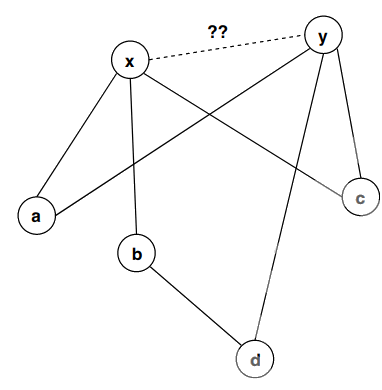
\includegraphics[width=7cm, keepaspectratio]{capitoli/methods/imgs/img6.png}
    \caption{An example illustrating the cycle formation link probability model.}
\end{figure}

Consider a cycle formation model ( \(CF (k)\) ) of degree \((k = 3)\).
The Seed link \((x, y)\), here, can be generated by the following three
mechanisms: - \texttt{random\ link\ occurrence\ g(1)} -
\texttt{length-2\ cycle\ generation\ g(2)}
i.e.~\((x −a −y and x −c −y)\) -
\texttt{length-4\ cycle\ generation\ g(3)} i.e.~\((x −b −d −y)\).

The main issue is to combine several generation mechanisms to compute
total link occurrence probability. The author posits a method to combine
both path and cycle (of different lengths) generation mechanism in the
framework. The expected general clustering coefficient of degree \(k\)
for this model can be estimated as
\[E[C(k)] = f(c_1, c_2, ..., c_k) = \sum_{i} |G_i|p(G_i)p((e_{l, k+1} \in E|G_i)) \]
where \(|G_i|\) is the number of subgraph possible corresponding to the
graph pattern \(G_i\), \(p(G_i)\) is the probability of occurrence of
one of such graphs \(G_i\), and \(p(e_{l,k+l})\) is the probability of
edge \(e_{l,l+1}\) to occur given the pattern \(G_i\). Finally, given
the coefficients, the probability of existence of link is
\[p_{x,y}(c_1, ..., c_k) = \frac{c_1 \prod_{i=2}^{k} c_i^{|path^i_{x,y}|}}{c_1 \prod_{i=2}^{k} c_i^{|path^i_{x,y}|} + (1-c_1)\prod_{i=2}^{k} (1-c_i)^{|path^i_{x,y}|}}\]

\textbf{Liu et al.} proposed degree related clustering coefficient to
quantify the clustering ability of nodes. They applied the same to paths
of shorter lengths and introduced a new index
\texttt{Degree\ related\ Clustering\ ability\ Path\ (DCP)}. They
performed the \texttt{degree\ of\ robustness\ (DR)} test for their index
and showed that missing links have a small effect on the index. Recently
\textbf{Wu et al.} extracted triangle structure information in the form
of node clustering coefficient of common neighbors. Their experiments on
several real datasets show comparable results to the \texttt{CAR} index.
The same concept of the clustering coefficient also introduced in the
work presented by \textbf{Wu et al.}. Authors introduce both node and
link clustering information in their work. Their experiments on
different network datasets showed better performance results against
existing methods, especially on middle and large network datasets.
\textbf{Kumar et al.} explored the concept of node clustering
coefficient to the next level (level-2) that captures more clustering
information of a network. The comprehensive results on several
real-world datasets show better performance compared to local methods
and comparable to the node embedding method \texttt{Node2vec}.
Meanwhile, \textbf{Benson et al.} studied simplicial closure events to
capture higher-order structures in several temporal networks. The
simplicial closure events are the process of closure of timestamped
simplices (simplicial complexes 2 are set of nodes with different sizes)
available in a dataset. These structures are common in several real-time
complex systems, for example, communication in a group, collaboration of
authors for a paper, etc. To assess these higher-order structures, the
authors study the simplicial closure events on triples of nodes (for
simplicity) and suggest that the open triangles or triples of nodes with
strong ties are more likely to close in the future.

\subsection{Structural Perturbation Method}

\textbf{\emph{Lu et al.}} introduced a new framework of computing
predictability of links in the networks. They coined a
\textbf{structural consistency index} to quantify the link
predictability. This index is based on the assumption that ``\emph{links
    in a network are highly predictable if no significant changes occur in
    the structural feature after the addition or deletion of a small
    fraction of the link}''. Based on this index, they proposed a new
similarity index, namely
\texttt{structural\ perturbation\ method\ (SPM)}. The experimental
results show the outstanding performance compared to the
state-of-the-art in their paper.


%% Aggiungere i capitoli qui sotto
\chapter{Existing Methods \normalfont{\emoji{bookmark-tabs}}}

Recently, numerous methodologies of link prediction have been
implemented. These methods can be grouped into several categories, like
\textbf{similarity-based, probabilistic models, learning-based models},
etc.

\begin{figure}[H]
    \centering
    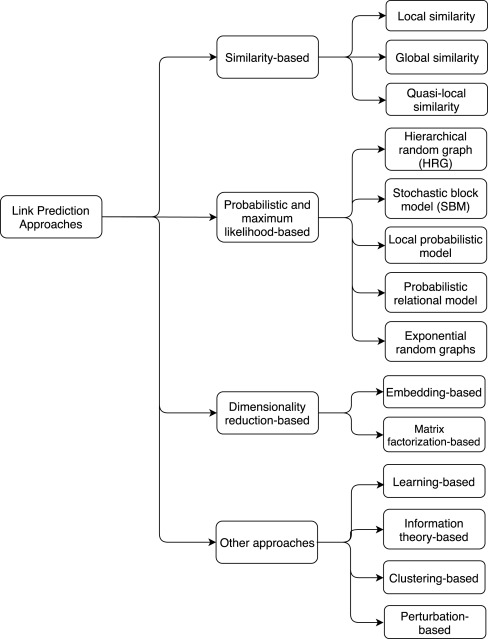
\includegraphics[width=9cm, keepaspectratio]{capitoli/methods/imgs/img2.jpg}
\end{figure}

\section{Similarity-based Methods}

Similarity-based metrics are the simplest one in link prediction, in
which for each pair \(x\) and \(y\), a similarity score \(S(x, y)\) is
calculated. The score \(S(x, y)\) is based on the structural or node's
properties of the considered pair. The non-observed links (i.e.,
\(U - E^T\) ) are assigned scores according to their similarities.
\textbf{The pair of nodes having a higher score represents the predicted
    link between them}. The similarity measures between every pair \emph{can
    be calculated using several properties of the network}, one of which is
structural property. Scores based on this property can be grouped in
several categories like \textbf{local and global}, and so on.

\subsection{Local similarity indices}

Local indices are generally calculated using information about common
neighbors and node degree. These indices \textbf{consider immediate
    neighbors of a node}. The following are some examples of local
similarity indices with a description and method to calculate them:

\begin{itemize}
    \item \texttt{Common\ Neighbors\ (CN)}: In a given network or graph, the size
          of common neighbors for a given pair of nodes \(x\) and \(y\) is
          calculated as the size of the intersection of the two nodes
          neighborhoods ( \(\Gamma\) ). \[S(x, y) = |\Gamma(x) \cap \Gamma(y)|\]
          The likelihood of the existence of a link between x and y increases with
          the number of common neighbors between them.
    \item \texttt{Jaccard\ Coefficient}: This metric is similar to the Common
          Neighbors. Additionally, it normalizes the above score, as given below:
          \[S(x, y) = \frac{|\Gamma(x) \cap \Gamma(y)|}{|\Gamma(x) \cup \Gamma(y)|}\]
          The Jaccard coefficient is defined as the probability of selection of
          common neighbors of pairwise vertices from all the neighbors of either
          vertex. The pairwise Jaccard score increases with the number of common
          neighbors between the two vertices considered. Some researcher
          (\textbf{Liben-Nowell et al.}) demonstrated that this similarity metric
          \textbf{performs worse} as compared to Common Neighbors.
    \item \texttt{Adamic/Adar\ Index\ (AA)}: Adamic and Adar presented a metric to
          calculate a similarity score between two web pages based on shared
          features, which are further used in link prediction after some
          modification
          \[S(x, y) = \sum_{z \in \Gamma(x) \cap \Gamma(y)} \frac{1}{log k_z}\]
          where \(k_z\) is the degree of the node \(z\). It is clear from the
          equation that more weights are assigned to the common neighbors having
          smaller degrees. This is also intuitive in the real-world scenario, for
          example, a person with more number of friends spend less time/resource
          with an individual friend as compared to the less number of friends.
    \item \texttt{Preferential\ Attachment\ (PA)}: The idea of preferential
          attachment is applied to generate a growing scale-free network. The term
          \textbf{growing} represents the incremental nature of nodes over time in
          the network. The likelihood incrementing new connection associated with
          a node \(x\) is proportional to \(k_x\) , the degree of the node.
          Preferential attachment score between two nodes x and y can be computed
          as: \[S(x, y) = k_x k_y\] This index shows the worst performance on most
          networks. The \textbf{simplicity} (as it requires the least information
          for the score calculation) and the \textbf{computational time} of this
          metric are the main advantages. PA shows better results if larger degree
          nodes are densely connected, and lower degree nodes are rarely
          connected. In the above equation, summation can also be used instead of
          multiplication as an aggregate function.
    \item \texttt{Resource\ Allocation\ Index\ (RA)}: Consider two non-adjacent
          vertices \(x\) and \(y\). Suppose node \(x\) sends some resources to
          \(y\) through the common nodes of both \(x\) and \(y\) then the
          similarity between the two vertices is computed in terms of
          \textbf{resources sent} from \(x\) to \(y\). This is expressed
          mathematically as:
          \[S(x, y) = \sum_{z \in \Gamma(x) \cap \Gamma(y)} \frac{1}{k_z}\] The
          difference between \textbf{RA} and \textbf{AA} is that the RA index
          heavily penalizes to higher degree nodes compared to the AA index.
          Prediction results of these indices become almost the same for smaller
          average degree networks. This index shows good performance on
          heterogeneous networks with a high clustering coefficient, especially on
          transportation networks.
    \item \texttt{Cosine\ similarity\ or\ Salton\ Index\ (SI)}: This similarity
          index between two records (documents) is measured by calculating the
          Cosine of the angle between them. The metric is all about the
          orientation and not magnitude. The Cosine similarity can be computed as
          \[S(x, y) = \frac{|\Gamma(x) \cap \Gamma(y)|}{\sqrt{(k_x k_y)}}\] -
          \texttt{Sorensen\ Index}: It is very similar to the Jaccard index.
          \textbf{McCune et al.} show that it \textbf{is more robust than Jaccard
              against the outliers}.
          \[S(x, y) = \frac{2|\Gamma(x) \cap \Gamma(y)|}{k_X + k_y}\]
    \item \texttt{CAR-based\ Common\ Neighbor\ Index\ (CAR)}: CAR-based indices
          are presented based on the assumption that the link existence between
          two nodes is more likely if their common neighbors are members of a
          local community (local-community-paradigm (LCP) theory). In other words,
          the likelihood existence increases with the number of links among the
          common neighbors (local community links (LCLs)) of the seed node pair as
          described in the following figure.
          \[S(x, y) = CN(x, y) \text{ x } LCL(x, y) = CN(x, y) \text{ x } \sum_{z \in \Gamma(x) \cap \Gamma(y)} \frac{|\gamma(z)|}{2} \]
          where \(CN(x, y) = |\Gamma(x) ∩ \Gamma(y)|\) is number of common
          neighbors. \(LCL(x, y)\) refers to the number of local community links
          which are defined as the links among the common neighbors of seed nodes
          x and y. \(\gamma(z)\) is the subset of neighbors of node \(z\) that are
          also common neighbors of \(x\) and \(y\).

          \begin{figure}[H]
              \centering
              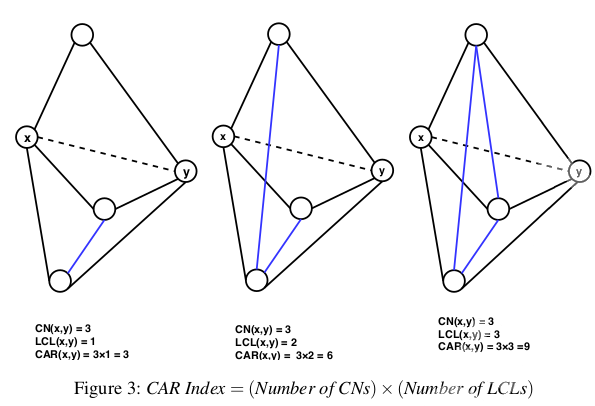
\includegraphics[width=8cm, keepaspectratio]{capitoli/methods/imgs/img3.png}
          \end{figure}
    \item \texttt{CAR-based\ Adamic/Adar\ Index\ (CAA)}: If \(LCL\) is considered
          as an accuracy enhancer, then the \(CAA\) index is obtained by
          incorporating the \(LCL\) theory to the well known AA index and
          mathematically expressed by the equation given below.
          \[S(x, y) = \sum_{z \in \Gamma(x) \cap \Gamma(y)} \frac{|\gamma(z)|}{\log_2(k_z)} \]
    \item \texttt{CAR-based\ Resource\ Allocation\ Index\ (CRA)}: Is a general
          application of the LCL theory to other indices and generate the CRA
          index by incorporating this concept into the existing RA index of the
          literature. Mathematically, the CRA can be expressed as
          \[S(x, y) = \sum_{z \in \Gamma(x) \cap \Gamma(y)} \frac{|\gamma(z)|}{k_z}\]
    \item \texttt{CAR-based\ Preferential\ Attachment\ Index\ (CPA)}: This is
          the preferential attachment index based on the CAR index. CPA is
          obtained by incorporating the LCL theory to the original PA method and
          expressed mathematically by
          \[S(x, y) = e_x e_y + e_x CAR(x, y) + e_y CAR(x, y) + CAR(x, y)^2\]
          where \(e_x\) is the number of neighbors of \(x\) not shared by \(y\)
          and \(CAR(x, y)\) is the similarity score of the node pair \(x\) and
          \(y\) using CAR index. CAR-based methods listed above show the best
          performance on LCP networks. The LCP networks are related to dynamic and
          heterogeneous systems and facilitate network evolution of social and
          biological networks.
    \item \texttt{Hub\ Promoted\ Index\ (HPI)}: This
          similarity index promotes the formation of links between the sparsely
          connected nodes and hubs. It also tries to prevent links formation
          between the hub nodes. This similarity metric can be expressed
          mathematically as
          \[S(x, y) = \frac{|\Gamma(x) \cap \Gamma(y)|}{min(k_x, k_y)}\]
    \item \texttt{Hub\ Depressed\ Index\ (HDI)}: This index is the same as the
          previous one but with the opposite goal as it avoids the formation of
          links between hubs and low degree nodes in the networks. The Hub
          depressed index promotes the links evolution between the hubs as well as
          the low degree nodes. The mathematical expression for this index is
          given below.
          \[S(x, y) = \frac{|\Gamma(x) \cap \Gamma(y)|}{max(k_x, k_y)}\]
    \item \texttt{Local\ Naive\ Bayes-based\ Common\ Neighbors\ (LNBCN)}: The
          above similarity indices are somehow based on common neighbors of the
          node pair where each of the which are equally weighted. This method is
          based on the Naive Bayes theory and arguments that different common
          neighbors play different role in the network and hence contributes
          differently to the score function computed for non-observed node pairs
          \[S(x, y) = \sum_{z \in \Gamma(x) \cap \Gamma(y)} [log(\frac{C(z)}{1 - C(z)}) + log(\frac{1 - \rho}{\rho})]\]
          where \(C(z)\) is node clustering coefficient and \(\rho\) is the
          network density expressed as \[\rho = \frac{|E|}{n(n-1)/2}\]
    \item \texttt{Leicht-Holme-Newman\ Local\ Index\ (LHNL)}: The logic below this
          index is that two vertices are similar to each other if their
          corresponding neighbors are self-similar to themselves. This score is
          defined by the ratio of the path of length two that exits between two
          vertices and the expected path of the same length between them.
          \[S(x, y) = \frac{|\Gamma(x) \cap \Gamma(y)|}{k_x k_y}\]
    \item \texttt{Node\ Clustering\ Coefficient\ (CCLP)}: This index is also based
          on the clustering coefficient property of the network in which the
          clustering coefficients of all the common neighbors of a seed node pair
          are computed and summed to find the final similarity score of the pair.
          Mathematically \[S(x, y) = \sum_{z \in \Gamma(x) \cap \Gamma(y)} C(z)\]
          where \[C(z) = \frac{t(z)}{k_z(k_z - 1)}\] is clustering coefficient of
          the node \(z\) and \(t(z)\) is the total triangles passing through the
          node \(z\).
    \item \texttt{Node\ and\ Link\ Clustering\ coefficient\ (NLC)}:
          This similarity index is based on the basic topological feature of a
          network called ''\emph{Clustering Coefficient}''. The clustering
          coefficients of both nodes and links are incorporated to compute the
          similarity score.
          \[S(x, y) = \sum_{z \in \Gamma(x) \cap \Gamma(y)} \frac{|\Gamma(x) \cap \Gamma(z)|}{k_z -1} \text{ x }C(z) + \frac{|\Gamma(y) \cap \Gamma(z)|}{k_z -1} \text{ x }C(z)\]

\end{itemize}

\subsection{Global similarity indices}

Global indices are computed using entire topological information of a
network. The computational complexities of such methods are higher and
seem to be infeasible for large networks.

\begin{itemize}
    \item \texttt{Katz\ Index}: This
          index can be considered as a variant of the shortest path metric. It
          directly aggregates over all the paths between x and y and dumps
          exponentially for longer paths to penalize them. It can be expressed
          mathematically as:
          \[S(x, y) = \sum_{l = 1}^{\infty}\beta^l|paths_{x, y}^{<l>}| = \sum_{l = 1}^{\infty}\beta^l(A)^l_{x, y}\]
          where, \(paths_{x, y}^{<l>}\) is considered as the set of total \(l\)
          length paths between \(x\) and \(y\), \(\beta\) is a damping factor that
          controls the path weights and A is the adjacency matrix. For the
          convergence of above equation, \[\beta < \frac{1}{\lambda_1} \] where
          \(\lambda_1\) is the maximum eigenvalue of the matrix A. If 1 is added
          to each element of the diagonal of the resulting similarity matrix S,
          this expression can be written in matrix terms as \[S = \beta AS + I\]
          where \(I\) is the identity matrix of the proper dimension. The
          similarity between all pairs of nodes can be directly computed using the
          closed-form by rearranging for \(S\) in the previous expression and
          subtracting the previously added 1 to the elements in the diagonal. Katz
          score for each pair of nodes in the network is calculated by finding the
          similarity matrix as \[S = (I - \beta A)^{- 1} - I\] The computational
          complexity of the given metric is high, and it can be roughly estimated
          to be cubic complexity which is not feasible for a large network.
    \item \texttt{Random\ Walk\ with\ Restart\ (RWR)}: Let \(\alpha\) be a
          probability that a random walker iteratively moves to an arbitrary
          neighbor and returns to the same starting vertex with probability
          \((1 - \alpha)\). Consider \(q_{xy}\) to be the probability that a
          random walker who starts walking from vertex \(x\) and located at the
          vertex \(y\) in steady-state. Now, this probability of walker to reach
          the vertex \(y\) is expressed mathematically as
          \[\overrightarrow{q_x} = \alpha P^T \overrightarrow{q_x} + (1-\alpha) \overrightarrow{e_x}\]
          where \(\overrightarrow{e_x}\) is the seed vector of length \(|V|\)
          (i.e., the total number of vertices in the graph). This vector consists
          of zeros for all components except the elements \(x\) itself. The
          transition matrix \(P\) can be expressed as
          \[\overrightarrow{q_x} = (1-\alpha)(I - \alpha P^T)^{-1} \overrightarrow{e_x}\]
          Since this similarity is not symmetric, the final score between the node
          pair (x, y) can be computed as \[S(x, y) = q_{xy} + q_{yx}\] It is clear
          from the above equation that matrix inversion is required to solve,
          which is quite expensive and prohibitive for large networks.
    \item \texttt{Shortest\ Path}: The inverse relation between the similarity and
          length of the shortest path is captured by the following mathematical
          equation given below. \[S(x, y) = -|d(x, y)|\] where Dijkstra algorithm
          is applied to efficiently compute the shortest path d(x, y) between the
          node pair (x, y). The prediction accuracy of this index is low compared
          to most local indices.
    \item \texttt{Leicht-Holme-Newman\ Global\ Index\ (LHNG)}: This global index
          is based on the principle that two nodes are similar if either of them
          has an immediate neighbor, which is similar to the other node. This is a
          recursive definition of similarity where a termination condition is
          needed. The termination condition is introduced in terms of
          self-similarity, i.e., a node is similar to itself. Thus, the similarity
          score equation consists of two terms: first, the neighbor similarity,
          and the second, self-similarity, as given below.
          \[S(x, y) = \phi  \sum_z A_{x, z} S_{z, y} + \psi \delta_{x, y}\] Here,
          the first term is neighborhood similarity and the second term is
          self-similarity. \(\psi\) and \(\phi\) are free parameters that make a
          balance between these two terms. When the free parameter \(\psi\) = 1,
          this index resembles to the Katz index.
    \item \texttt{Cosine\ based\ on\ L+\ (Cos+)}: Laplacian matrix is extensively
          used as an alternative representation of graphs in spectral graph
          theory. This matrix can be defined as \(L = D - A\), where, \(D\) is the
          diagonal matrix consisting of the degrees of each node of the matrix and
          \(A\) is the adjacency matrix of the graph. The pseudo-inverse of the
          matrix defined by Moore-Penrose is represented as \(L^+\) and each entry
          of this matrix is used to represent the similarity score between the two
          corresponding nodes. The most common way to compute this pseudo-inverse
          is by computing the \textbf{singular value decomposition (SVD)} of the
          Laplacian matrix [$(L = U \Sigma V^{}T)$, where \(U\) and \(V\)
                  are left and right singular vectors of \(SVD\)] as follows
          \[L^+ = V \Sigma^+ U^T\] \(\Sigma^+\) is obtained by taking the inverse
          of each nonzero element of the \(\Sigma\). Further, the similarity
          between two nodes \(x\) and \(y\) can be computed using any inner
          product measure such as Cosine similarity given as
          \[S(x, y) = \frac{L_{x, y}^+}{\sqrt{L_{x, x}^+ L_{y, y}^+}}\]
    \item \texttt{Average\ Commute\ Time\ (ACT)}: This index is based on the
          random walk concept. A random walk is a Markov chain which describes the
          movements of a walker. It defined as the average number of
          movements/steps required by a random walker to reach the destination
          node \(y\), and come back to the starting node \(x\). If \(m(x, y)\) be
          the number of steps required by the walker to reach \(y\) from \(x\),
          then the following expression captures this concept.
          \[n(x, y) = |E| (l_{xx}^+ + l_{yy}^+ - 2l_{xy}^+) \] where \(l_{xy}^+\)
          denotes the \((x, y)\) entry of the matrix \(L^+\) . Pseudo-inverse of
          the Laplacian, \(L^+\) can be computed as
          \[L^+ = (L - \frac{ee^T}{n})^{-1} + \frac{ee^T}{n}\] where \(e\) is a
          column vector consisting of 1's. Smaller value of this equation will
          represent higher similarity. The final expression is the following
          \[S(x, y) = \frac{1}{l_{xx}^+ + l_{yy}^+ - 2l_{xy}^+}\]
    \item \texttt{Normalized\ Average\ Commute\ Time\ (NACT)}: This is a variant
          of ACT that takes into account node degrees. For a high degree node
          (hub) \(y\), \(m(x, y)\) is usually small regardless of \(x\), the
          similarity measure is normalized with stationary distribution \(\pi\) of
          the Markov chain describing random walker on the graph. This normalized
          measure can be computed with the following equation
          \[S(x, y) = \frac{1}{(m(x, y)\pi_y + m(y, x)\pi_x)}\]
    \item \texttt{Matrix\ Forest\ Index\ (MF)}: his index is based on the concept
          of spanning tree which is defined as the subgraph that spans total nodes
          without forming any cycle. The spanning tree may contain total or less
          number of links as compared to the original graph. Chebotarev and Shamis
          proposed a theorem called matrix-forest theorem which states that the
          number of spanning tree in a graph is equal to the co-factor of any
          entry of Laplacian matrix of the graph. Here, the term forest represents
          the union of all rooted disjoint spanning trees. The similarity between
          two nodes \(x\) and \(y\) can be computed with the equation given below
          \[S = (I + L)^{-1}\] where \((I + L)\_{(x,y)}\) is the number of
          spanning rooted forests ( \(x\) as root ) consisting of both the nodes
          \(x\) and \(y\). Moreover, this quantity is equal to the co-factor of
          \((I + L)_{(x,y)}\) .
    \item \texttt{SimRank}: This is a measure of
          structural context similarity and shows object-to-object relationships.
          It is not domain-specific and recommends to apply in directed or mixed
          networks. The basic assumption of this measure is that two objects are
          similar if they are related to similar objects. SimRank computes how
          soon two random walkers meet each other, starting from two different
          positions. This measure can be represented in matrix form as
          \[S(x,y) = \alpha W^T SW + (1 - \alpha)I\] where, \(\alpha \in (0, 1)\)
          is a constant. \(W\) is the transformation matrix and computed by
          normalizing each column of adjacency matrix \(A\) as
          \[
              W_{ij} = \frac{a_{ij}}{\sum_{k=1}^{n}}
          \]
          The computational complexity
          of this measure is high for a large network, and to reduce its time, the
          authors suggest pruning recursive branches.
    \item \texttt{Rooted\ Pagerank\ (RPR)}: The idea of PageRank was originally
          proposed to rank the web pages based on the importance of those pages.
          The algorithm is based on the assumption that a random walker randomly
          goes to a web page with probability \(\alpha\) and follows hyper-link
          embedded in the page with probability \((1 - \alpha)\). Chung et
          al.~used this concept incorporated with a random walk in link prediction
          framework. The importance of web pages, in a random walk, can be
          replaced by stationary distribution. The similarity between two vertices
          \(x\) and \(y\) can be measured by the stationary probability of \(y\)
          from \(x\) in a random walk where the walker moves to an arbitrary
          neighboring vertex with probability \(\alpha\) and returns to \(x\) with
          probability \((1 - \alpha)\). Mathematically, this score can be computed
          for all pair of vertices as
          \[RPR = (1 - \alpha)(I - \alpha \hat{N})^{-1}\] where
          \(\hat{N} = D^{-1} A\) is the normalized adjacency matrix with the
          diagonal degree matrix \(D[i, i] = \sum_j A[i, j]\).
\end{itemize}

\subsection{Quasi-local indices}

Quasi-local indices have been introduced as a trade-off between local
and global approaches or performance and complexity. These metrics are
as efficient to compute as local indices. Some of these indices extract
the entire topological information of the network. The time complexities
of these indices are still below compared to the global approaches.

\begin{itemize}
    \item \texttt{Local\ Path\ Index\ (LP)}: This metric has the intent to furnish
          a good trade-off between accuracy and computational complexity. The
          metric is expressed mathematically as \[S^{LP} = A^2 + \epsilon A^3\]
          where $\epsilon$ represents a free parameter. Clearly, the measurement
          converges to common neighbor when \(\epsilon = 0\). If there is no
          direct connection between \(x\) and \(y\), \((A^3)_{xy}\) is equated to
          the total different paths of length 3 between \(x\) and \(y\). The index
          can also be expanded to generalized form
          \[S^{LP} = A^2 + \epsilon A^3 + \epsilon^2 A^4 + ... + \epsilon^{(n−2)} A^n\]
          where \(n\) is the maximal order. Computing this index becomes more
          complicated with the increasing value of \(n\). The LP index outperforms
          the proximity-based indices, such as RA, AA, and CN.
    \item \texttt{Path\ of\ Length\ 3\ (L3)}: Georg Simmel, a German sociologist,
          first coined the concept ``triadic closure'' and made popular by Mark
          Granovetter in his work ``\emph{The Strength of Weak Ties}''. The
          authors proposed a similarity index in protein-protein interaction (PPI)
          network, called \textbf{\emph{path of length 3 (or L3)}} published in
          the Nature Communication. They experimentally show that the triadic
          closure principle (TCP) does not work well with PPI networks. They
          showed the paradoxical behavior of the TCP (i.e., the path of length 2),
          which does not follow the structural and evolutionary mechanism that
          governs protein interaction. The TCP predicts well to the interaction of
          self-interaction proteins (SIPs), which are very small (4\%) in PPI
          networks and fails in prediction between SIP and non SIP that amounts to
          96\%. They showed that the L3 index performs well in such conditions and
          give mathematical expression to compute this index as
          \[S(x, y) = \sum \frac{a_{x,u} a_{u,v} a_{v,y}}{k_u k_v}\]
    \item \texttt{Similarity\ based\ on\ Local\ Random\ Walk\ and\ Superposed\ Random\ Walk\ (LRW\ and\ SRW)}:
          This metric propose a new similarity measures by exploiting the random
          walk concept on graphs with limited walk steps. They defined node
          similarity based on random walks of lower computational complexity
          compared to the other random walk based methods. Given a random walker,
          starting from the node \(x\), the probability of reaching the random
          walker to the node \(y\) in \(t\) steps is
          \[\overrightarrow{\pi}\_x(t) = P^T \overrightarrow{\pi}\_x(t-1)\] where
          \(\overrightarrow{\pi}\_x(0)\) is a column vector with \(x^{th}\)
          element as 1 while others are 0's and \(P^T\) is the transpose of the
          transition probability matrix \(P\). \(P_{xy}\) entry of this matrix
          defines the probability of a random walker at node \(x\) will move to
          the next node \(y\). It is expressed as \(P_{xy} = \frac{a_{kx}}{k_x}\)
          , where \(a_{xy}\) is 1 when there is a link between \(x\) and \(y\) and
          0, otherwise. The authors computed the similarity score ( \(LRW\) )
          between two nodes based on the above concept as
          \[S^{LRW}(x, y) = \frac{k_x}{2|E|}\pi_{xy}(t) + \frac{k_y}{2|E|}\pi_{xy}(t)\]
          This similarity measure focus on only few steps covered by the random
          walker (hence quasi-local) and not the stationary state compared to
          other approaches. Random walk based methods suffer from the situation
          where a random walker moves far away with a certain probability from the
          target node whether the target node is closer or not. This is an obvious
          problem in social networks that show a high clustering index i.e.,
          clustering property of the social networks. This degrades the similarity
          score between the two nodes and results in low prediction accuracy. One
          way to counter this problem is that continuously release the walkers at
          the starting point, which results in a higher similarity between the
          target node and the nearby nodes. By superposing the contribution of
          each walker (walkers move independently), SRW is expressed as
          \[S^{SRW} (x, y) (t) = \sum_{l=1}^{t} S^{LRW} (l)\]
\end{itemize}

\subsection{Some Remarks}

Similarity-based approaches mostly focus on the structural properties of
the networks to compute the similarity score. \textbf{\emph{Local
        approaches}} consider, in general, neighborhood information (direct
neighbors or neighbors of neighbor), which take less time for
computation. This is the property that makes the local approaches
feasible for massive real-world network datasets. \textbf{\emph{Global
        approaches}} consider the entire structural information of the network;
that is why time required to capture this information is more than local
and quasi-local approaches. Also, sometimes, entire topological
information may not be available at the time of computation, especially
in a decentralized environment. So, parallelization over the global
approaches may not possible or very complex compared to the local and
quasi-local approaches. The performance or prediction accuracy of these
approaches (i.e., global approaches) is better compared to local and
quasi-local. \textbf{\emph{Quasi-local approaches}} extract more
structural information than local and somehow less information compared
to the global.


\section{Probabilistic and maximum likelihood models}

For a given network \(G(V, E)\), \textbf{\emph{the probabilistic model
        optimizes an objective function to set up a model that is composed of
        several parameters}}. Observed data of the given network can be
estimated by this model nicely. At that point, the likelihood of the
presence of a non-existing link \((i, j)\) is evaluated using
conditional probability \(P(A_{i j} = 1 | \Theta )\). Several
\texttt{probabilistic\ models} and \texttt{maximum\ likelihood\ models}
have been proposed in the literature to \textbf{infer missing links in
    the networks}.\\

\textbf{The probabilistic models normally require more information like
    node or edge attribute knowledge in addition to structural information}
Extracting these attribute information is not easy; moreover, the
parameter tuning is also a big deal in such models that limit their
applicability. \emph{Maximum likelihood methods are complex and
    time-consuming}, so these models are not suitable for real large
networks.

\subsection{Local probabilistic model for link prediction}

\textbf{Wang et al.} proposed a \texttt{local\ probabilistic\ model} for
link prediction in an \emph{undirected network}. They employed three
different types of features viz., topological, semantic, and
cooccurrence probability features extracted from different sources of
information.\\

They presented an idea of a central neighborhood set derived from the
local topology of the considered node-pair, which is relevant
information for the estimation of a link between them. They computed
non-derivable frequent itemsets (i.e., those itemsets whose occurrence
statistics can not be derived from other itemset patterns) from the
network events log data, which is further used as training data for the
model. An event corresponds to a publication of a paper (i.e., authors'
interactions in the paper is a an event, and a set of such events is the
event log) in the Coauthorship network. The model is shown in the
following Figure, which considers the approach described below.\\

First, the central neighborhood set between \(x\) and \(y\) is
calculated based on local event log data. One of the usual ways to find
the central neighborhood set is to find the \textbf{shortest path
    between two vertices of specified length}, and the vertices are lying on
this path can be included in the required set. There can be more than
one shortest path between two vertices, so more neighborhood sets can be
possible. Neighborhood sets of shorter lengths and more frequent
(frequency score is used when more shortest paths of the same length are
available) are chosen for the central neighborhood set. The authors
considered the shortest path up to length 4 since the nodes lying on the
shorter length path are more relevant.\\

In the second step, for a given central neighborhood set, non-derivable
frequent itemsets are used to learn the local probabilistic model.
\textbf{Calders et al.} proposed a depth-first search method to
calculate non-derivable itemsets and the same algorithm used by the
authors. Why non-derivable frequent itemsets? \textbf{Pavlov et al.}
first introduced the concept of frequent itemset to construct an
\texttt{MRF}. They argued that a \(K-itemset\) and its support
represents a \(K-way\) statistics, which can be viewed as a constraint
on the true underlying distribution that generates the data. Given a set
of itemset constraints, a maximum entropy distribution satisfying all
these constraints is selected as the estimate for the true underlying
distribution. This maximum entropy distribution is equivalent to an
\texttt{MRF}. Since the number formed links are very few compared to all
possible links in a sparse network, the authors used a support threshold
of one to extract all frequent itemsets. Theses extracted itemsets are
large in number that results in expensive learning for the \texttt{MRF}.
To reduce this cost, only non-derivable itemsets are extracted. They
find all such itemsets that lie entirely within the central neighborhood
set. Using these itemsets, a \texttt{Markov\ Random\ Field} is
\textbf{learned}.\\

In the last step, the \texttt{iterative\ scaling\ algorithm} is used to
learn a local \texttt{MRF} for the given central neighborhood set. This
process continues overall itemset constraints and continuously updates
the model until the model converges. Once the model learning process is
over, one can infer the co-occurrence probability by computing the
marginal probability over the constructed model. The
\texttt{Junction\ tree\ inference\ algorithm} is used to infer
co-occurrence probability. The algorithm to induce co-occurrence
probability feature for a pair of vertices can be found in
\href{https://static.aminer.org/pdf/PDF/000/303/209a_parameterized_probabilistic_model_of_network_evolution_for_supervised_link.pdf}{Local
    Probabilistic Models for Link Prediction}.

\subsection{Probabilistic relational model for link prediction (PRM)}

Existing works show that \textbf{node attributes play a significant role
    to improve the link prediction accuracy}. However, \textbf{no generic
    framework is available to incorporate node and link attributes} and
hence, not applicable to all scenarios. To this end, \textbf{the
    probabilistic model is a good and concrete solution that provides a
    systematic approach to incorporate both node and link attributes in the
    link prediction framework}. Pioneering works on \texttt{PRM} include
\textbf{Getoor et al.} study on directed networks, \textbf{Taskar et
    al.} study on undirected networks, \textbf{Jennifer Neville}
work on for both networks, etc. published in \texttt{JMLR} is based on
\texttt{Relational\ Bayesian\ network\ (RBN)} where relation links are
directed and published in NIPS is based on
\texttt{Relational\ Markov\ network\ (RMN)} where relational links are
undirected.\\

\texttt{PRM} was originally designed for attribute prediction in
relational data, and it later extended to link prediction task. The
authors employed the attribute prediction framework to link prediction.
This casting can be understood with the following example: - Consider
the problem of link prediction in a coauthorship network. Non-relational
frameworks of link prediction consider only one entity type
``\emph{person}'' as node and one relationship; however, relational
framework (\texttt{PRMs}) include more entity types like article,
conference venue, institution, etc. Each entity can have attributes like
a person (attributes: name, affiliation institute, status (student,
professor)), article (attributes: publication year, type (regular,
review)), etc. Several relational links may possible among these
entities like advisor-advisee/research scholar relation between two
persons, author relationship between person and paper entities, and
paper can be related to the conference venue with publish relationship.
Moreover, relationships (links) among these entities can also have
attributes viz., exists (if there is a link between the two involved
entities), or not-exist (no link between the involved entities). This
way, the link prediction can be reduced to an attribute prediction
framework/model.\\

During the model training, a single link graph is constructed that
incorporates above heterogeneous entities and relationships among them.
Model parameters are estimated discriminatively to maximize the
probability of the link existence and other parameters with the given
graph attribute information. The learned model is then applied using
probabilistic inference to predict missing links.\\

\subsection{Hierarchical structure model (HSM)}

These models are based on the assumption that the structures of many
real networks are hierarchically organized, where nodes are divided into
groups, which are further subdivided into subgroups and so forth over
multiple scales. Some representative work systematically encodes such
structures from network data to build a model that estimates model
parameters using statistical methods. These parameters are then used in
estimating the link formation probability of unobserved links.\\

Some studies suggest that many real networks, like biochemical networks
(protein interaction networks, metabolic networks, or genetic regulatory
networks), Internet domains, etc. are hierarchically structured. In
hierarchical networks, vertices are divided into groups, which are
further sub-divided into subgroups and so forth over multiple scales.
\textbf{Clauset et al.} proposed a probabilistic model that takes a
hierarchical structure of the network into account. The model infers
hierarchical information from the network data and further applies it to
predict missing links.\\

The hierarchical structures are represented using a tree (binary), or
dendrogram, where, the leaves (i.e., \(n\) ) represent the number of
total vertices in the network and each internal vertex out of (
\(n - 1\) ) corresponds to the group of vertices descended from it. Each
internal vertex \(r\) is associated with a probability \(p_r\) , then
the existing edge probability \(p_{xy}\) between two vertices \(x\) and
\(y\) is given by \(p_{xy} = p_r\) where, \(r\) is their lowest common
ancestor. The hierarchical random graph is then, represented by the
dendrogram \(D^{\star}\) with the set of probability \(\{ p_r \}\) as
\(\left( D^{\star},\{p_r\} \right)\). Now the learning task is to find
the hierarchical random graph(s) that best estimates the observed
real-world network data. Assuming all possible dendrograms to be equally
likely, Bayes theorem says that the probability of the dendrogram
\(\left(D^{\star}, \{p_r\} \right)\) that best estimates the data is
proportional to the posterior probability or likelihood, \(L\) from
which the model generates the observed network and our goal is to
maximize \(L\) . The likelihood of a hierarchical random graph
\(\left(D^{\star},\{p_r\} \right)\) is computed using the following
equation

\[
    L(D^{\star}, \{p_r\}) = \prod_{r \in D^{\star}} p_r^{E_r} (1-p_r)^{L_r R_r - Er},
\]

where \(L_r\) and \(R_r\) are the left and right subtree rooted at
\(r\), and \(E_r\) is the number of links in the network whose endpoints
have \(r\) as their lowest common ancestor in \(D^{\star}\) . The above
equation assumes the convention \(0^0 = 1\). For a given dendrogram
\(D^{\star}\) , it is easy to compute the probability \(p_r\) that
maximizes \(L(D^{\star}, \{p_r\})\) i.e.

\[
    \overline{p_r} = \frac{E_r}{L_r R_r}.
\]

This can be understood with the following example illustrated in the
next Figure. Now, this model can be used to estimate the missing links
of the network as follows. Sample a large number of dendrograms with
probability proportional to their likelihood. Then, compute the mean
connecting probability \(\overline{p_{xy}}\) of each nonexisting pair
\((x, y)\) by averaging the corresponding probability \(p_{xy}\) overall
sampled dendrograms. Sort these vertices pairs scores in descending
order and selects top-l links to be predicted.

\begin{figure}[H]
    \centering
    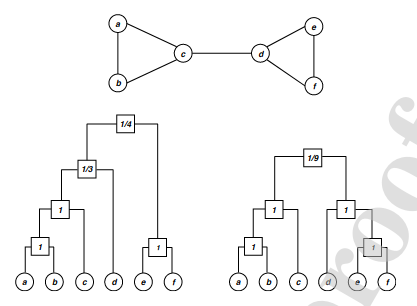
\includegraphics[width=8cm, keepaspectratio]{capitoli/methods/imgs/img8.png}
    \caption{ An illustrating example of \texttt{HSM} for a graph of 6 nodes and its
        two possible dendrograms. The internal nodes of each dendrogram are
        labeled as the maximum likelihood probability \(\overline{p}_r\). The
        likelihoods of the left and the right dendrograms are
        \(L(D1) = (1/3)(2/3)^2 (1/4)^2(3/4)^6\) \(= 0.00165\), and
        \(L(D2) = (1/9)(8/9)^8 = 0.0433\). Thus, the second (i.e., right)
        dendrogram is most probable as it divides the network in a balanced one
        at the first level.}
\end{figure}

\subsection{Stochastic block model (SMB)}

Hierarchical structures may not represent most networks. A more general
approach to represent these networks is block model where vertices are
distributed (partitioned) into blocks or communities and the connecting
probability between two vertices depends on blocks they belong to.
\textbf{Guimera et al.} presented a novel framework where stochastic
block model representation of a network is employed to find missing and
spurious links. The authors compute the reliability of the existence of
links given an observed network that is further used to find missing
links (non-existing links with higher reliabilities) and spurious links
(existing links with lower probabilities).\\

The link reliability \(R_{xy}\) between the two vertices \(x\) and \(y\)
is

\[R_{xy} = p_{BM} (A_{xy} = 1 | A^0).\]

i.e.~probability that the link truly exists given the observed network
\(A^0\), the block model \(BM\).\\

Generally, complex networks are outcomes of combination of mechanisms,
including modularity, role structure, and other factors. In \(SBM\),
partitioning vertices of network based on these mechanisms may result in
different block models that capture different correlations (patterns) of
the network. Assume that no prior knowledge of suitable models, the
reliability is expressed as

\[
    R_{xy} = \frac{1}{Z} \sum_{P \in P^{\star}} \left( \frac{l^{0}_{\sigma_x \sigma_y} + 1}{r^{0}_{\sigma_x \sigma_y + 2}} \right) \text{ exp } \left[ -H(P) \right],
\]

where the sum is over all possible partitions \(P^{\star}\) of the
network into groups, \(\sigma_x\) and \(\sigma_y\) are vertices \(x\)
and \(y\) groups in partition \(P\) respectively. Moreover, \(l^0_1\)
and \(r^0_{\sigma_{\alpha} \sigma_{\beta}}\) are the number of links and
maximum possible links in the observed network between groups \(\alpha\)
and \(\beta\) . The function \(H(P)\) is

\[H(P) = \sum_{\alpha \leq \beta} \left[ \ln \left( r_{\alpha \beta} \right) + \ln \binom {r_{\alpha \beta}}{l^0_{\alpha \beta}} \right],\]

and \(Z = \sum_{P \in P^{\star}} \text{ exp } \left[ -H(P) \right]\).\\

Practically, solving equation \(R_{xy} = \ldots\) , i.e., summing over
all possible partitions is too complex even for a small network.
However, the Metropolis algorithm can be used to correctly sample the
relevant partitions and obtain link reliability estimates.\\

The authors employed the link reliability concept to find missing links
and to identify the spurious link in the networks with the following
procedure.

\begin{itemize}
    \item
          \((i)\) Generate the observed network \(A^0\) by removing/adding some
          random links (for finding missing/spurious links) from/to the true
          network \(A^t\) .
    \item
          \((ii)\) Compute the link reliability for non-observed links (i.e.
          non-existing \(+\) missing/spurious links).
    \item
          \((iii)\) Arrange these links with their reliability score in
          decreasing order and decide the top-l links as desired ones (i.e.,
          missing/spurious links).
\end{itemize}

Probabilistic and maximum likelihood methods extract useful features and
valuable correlation among the data using hierarchical and stochastic
block models, which result in significant improvements in prediction
results as compared to some similarity-based methods. However, these are
\textbf{quite complex and time-consuming even on small datasets} that
limit their applicability on large scale real-world network datasets.

\subsection{Exponential random graph model (ERGM) or P-star model}

\section{Link prediction using Dimensionality Reduction}

The curse of dimensionality is a well-known problem in machine learning.
Some researchers employ dimension reduction techniques to tackle the
above problem and apply it in the \textbf{link prediction} scenario.

\subsection{Embedding-based link prediction}

The network embedding is considered as a dimensionality reduction
technique in which higher \(D\) dimensional nodes (vertices) in the
graphs are mapped to a lower \(d\) (\(d << D\)) \textbf{dimensional
    representation (embedding)} space by preserving the node neighborhood
structures. In other words, \textbf{\emph{find the embedding of nodes to
        a lower d-dimensions such that similar nodes (in the original network)
        have similar embedding (in the representation space)}}.\\ In the Figure
below you can see an application example of a dimensionality reduction
technique to a graph that represent a social network.

\begin{figure}[H]
    \centering
    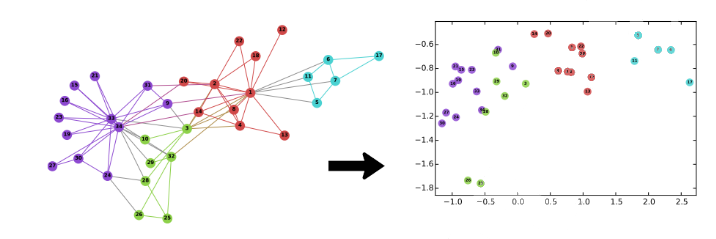
\includegraphics[width=12cm, keepaspectratio]{capitoli/methods/imgs/img4.png}
\end{figure}

The main component of the network embedding is the encoding function or
encoder \(f_{en}\) that map each node to the embedding space
\[f_{en}(x) = z_x\] where \(z_x\) is the \(d\)-dimensional embedding of
the node \(x\). The embedding matrix is \(Z \in R^{d x |V|}\), each
column of which represents an embedding vector of a node.\\

\begin{figure}[H]
    \centering
    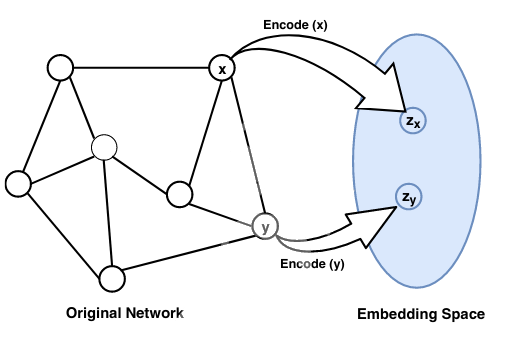
\includegraphics[width=10cm, keepaspectratio]{capitoli/methods/imgs/img5.png}
\end{figure}

Now, a similarity function is \(S(x, y)\) is defined that specifies how
to model the vector (embedding) space relationships equivalent to the
relationships in the original network, i.e.,
\[S(x, y) \approx z_x^T z_y\]

Here \(S(x, y)\) is the function that reconstructs pairwise similarity
values from the generated embedding. The term \(S(x, y)\) is the one
that differ according to the function used in different
factorization-based embedding approaches.\\

For example, \texttt{graph\ factorization} directly employ adjacency
matrix \(A\) i.e.~\((S(x, y) \overset{\Delta}{=} A_{(x,y)})\) to capture
first order proximity, \texttt{GraRep} selects
\((S(x, y) \overset{\Delta}{=} A^2_{(x,y)})\) and \texttt{HOPE} uses
other similarity measures(e.g. Jaccard neighborhood overlap). Most
embedding methods realize the reconstruction objective by minimizing the
loss function, L
\[L = \sum_{(x, y) \in \{V x V \}} l(z_x^T z_y, S(x, y))\]

Once the previous equation is \textbf{converged}
(i.e.~\textbf{trained}), one can use the trained encoder to generate
nodes embedding, which can further be employed to infer missing link and
other downstream machine learning tasks.\\

Recently, some network embedding techniques have been proposed and
applied successfully in link prediction problem. The
\texttt{Laplacian\ eigenmaps},
\texttt{Logically\ linear\ embedding\ (LLE)}, and \texttt{Isomap} are
examples based on the simple notion of embedding. Such embedding
techniques are having quite complex in nature and face scalability
issues. To tackle the scalability issue, graph embedding techniques have
leveraged the sparsity of real-world networks. For example,
\texttt{DeepWalk} extracts local information of truncated random walk
and embeds the nodes in representation space by considering the walk as
a sentence in the language model. It preserves higher order proximity by
maximizing the probability of co-occurrence of random walk of length
\(2k + 1\) (previous and next \(k\) nodes centered at a given node).
\texttt{Node2vec} also uses a random walk to preserves higher order
proximity but it is biased which is a trade-off between the
\texttt{breadth-first\ search\ (BFS)} and
\texttt{depth-first\ search\ (DFS)}.\\

The experimental results show that the \texttt{Node2vec} performs better
than the \texttt{Deepwalk}.\\

In next step, \textbf{Trouillon et al.} introduced complex embedding in
which simple matrix and tensor factorization have been used for link
prediction that uses a vector with complex values. Such composition of
complex embedding includes all possible binary relations especially
symmetric and anti-symmetric relations. Recently, some more studies have
been published in link prediction using embedding, for example,
\textbf{Cao et al.~subgraph embedding}, \textbf{Li et al.~deep dynamic
    network embedding}, \textbf{Kazemi et al.}, etc.

\subsection{Matrix factorization/decomposition-based link prediction}

From last decade, matrix factorization has been used in lots of papers
based on link prediction and recommendation systems. Typically, the
latent features are extracted and using these features, each vertex is
represented in latent space, and such representations are used in a
supervised or unsupervised framework for link prediction. To further
\textbf{improve the prediction results, some additional node/link or
    other attribute information can be used}. In most of the works,
non-negative matrix factorization has been used. Some authors also
applied the singular value decomposition technique. Let the input data
matrix is represented by \(X = (x_1, x_2, ..., x_n)\) that contains
\(n\) data vectors as columns. Now, factorization of this matrix can be
expressed as \[X \approx FG^T\] where
\(X \in R^{p x n}, F \in R^{p x k} , and G \in R^{n x k}\) . Here, \(F\)
contains the bases of the latent space and is called the basis matrix.
\(G\) contains combination of coefficients of the bases for
reconstructing the matrix \(X\) , and is called the coefficient matrix.
\(k\) is the dimension of latent space \((k < n)\). Several well-known
matrix factorizations are expressed based on some constraints on either
of the three matrices, for example

\begin{itemize}
    \item \texttt{SVD}:
          \(X_\pm \approx F_\pm G_\pm^T\)
    \item \texttt{NMF}:
          \(X_+ \approx F_+ G_+^T\)
    \item \texttt{Semi-NMF}:
          $X_\pm \approx F_\pm G_+\^{T} $
    \item \texttt{Convex-NMF}:
          $X_\pm \approx  X_\pm W_+ G_\pm^{T}$
\end{itemize}

In the above four equations, \(Z_\pm\) represents the nature of the
entries in the matrix \(Z\), i.e.~both positive and negative entries
allowed in the matrix \(Z\). In the last equation, \(F = XW\) represents
the convex combinations of the columns of \(F\) . Generally, such a
factorization problem can be modeled as the following
\texttt{Frobenius\ norm\ optimization\ problem}
\[min_{f, g} ||X - FG^T||^2_{fro}\]
\[\text{subject to} F \ge 0, G \ge 0\] Here \(||Z||^2_{fro}\) is the
frobenius norm of \(Z\) and the constraints represent NMF factorization.
However, any of the above four constraints can be used depending on the
requirement of the problem underlying. After solving the above
optimization problem, the similarity between a non-existing pair
\((x, y)\) can be computed by the similarity of the \(x^{th}\) and
\(y^{th}\) row vectors in the coefficient matrix \(G\).

\begin{itemize}
    % \tightlist
    \item
          \texttt{Acar\ et\ al.} expressed temporal link prediction as a matrix
          completion problem and solve it through the
          \texttt{matrix\ and\ tensor\ factorization}. They proposed a weighted
          method to collapsed the temporal data in a single matrix and factorize
          it using \texttt{CANDECOMP/PARAFAC\ (CP)} tensor decomposition method.
    \item
          \texttt{Ma\ et\ al.} also applied matrix factorization to temporal
          networks where features of each network are extracted using
          \texttt{graph\ communicability} and then collapsed into a single
          feature matrix using \texttt{weighted\ collapsing\ tensor\ (WCT)}.
          They showed the equivalence between eigen decomposition of
          \texttt{Katz\ matrix} and
          \texttt{non-negative\ matrix\ factorization\ (NMF)} of the
          communicability matrix that serves as the foundation of their
          framework.
    \item
          \texttt{Menon\ et\ al.} proposed a work for structural link
          prediction. Here, the problem is modeled as
          \texttt{matrix\ completion\ problem}, and
          \texttt{matrix\ factorization} are used to solve it. They introduced a
          supervised matrix decomposition framework that learns latent
          (unobserved) structural features of the graph and incorporates it with
          additional node/link explicit feature information to make a better
          prediction. Additionally, they allowed the factorization model to
          solve class imbalance problem by optimizing ranking loss.
    \item
          \texttt{Chen\ et\ al.} proposed a work, where the authors extracted
          topological matrix and attribute matrix and factorized these matrices
          using \texttt{non-negative\ matrix\ factorization}. The final score
          matrix is obtained by integrating these two matrices in the latent
          space.
\end{itemize}
\section{Other approaches}

\subsection{Learning-based frameworks for link prediction}

Earlier described approaches (e.g., similarity and probabilistic
methods) deal with the computing a score of each non-observed link
either by a similarity or a probabilistic function. However, \textbf{the
    link prediction problem can also be modeled as a learning-based model}
to exploit graph topological features and attribute information. The
problem is cast as a \textbf{supervised classification model} where a
\textbf{point} (i.e., training data) \textbf{corresponds to a
    vertex-pair in the network}, and the \textbf{label} of the point
\textbf{represents the presence or absence of an edge (link) between the
    pair}.\\ In other words, \emph{consider a vertex-pair} \(\mathit{(x, y)}\)
\emph{in the graph} \(\mathit{G(V, E)}\) \emph{and the label of the
    corresponding data point in the classification model is}
\(\mathit{l_{(x,y)}}\) . Then,

\[l_{(x, y)}=
    \begin{cases}
        +1 \ \text{ if } (x, y) \in E \\
        -1 \ \text{ if } (x, y) \notin E
    \end{cases}
\]

\textbf{This is typically a binary classification task} where several
classifiers (e.g.,
\texttt{decision\ tree,\ naive\ Bayes,\ support\ vector\ machine}, etc.)
can be employed to predict the label of unknown data points
(corresponding to missing links in the network). One of the major
challenges of this model (i.e., machine learning) is the
\textbf{selection of appropriate feature set}. Majority of the existing
research works extract feature sets from the network topology (i.e.,
topological information of the network). These \textbf{features are
    generic} and domain-independent that are \textbf{applicable to any
    network}. Such features are typical,
\texttt{neighborhood,\ and\ path-based\ features}.\\ Some other works
concentrate on extracting node and edge features that play a crucial
role to improve the performance of link prediction. The cost of
extraction of such features is cheap and easy, while the main
disadvantage is the domain-specific nature of them.

\subsection{Information theory-based link prediction}

Several complex networks have utilized the concept of
\textbf{information theory to compute their complexity on different
    scales}. They defined several correlation measures and modeled some
networks (e.g., \texttt{star,\ tree,\ lattice,\ ER\ graph}, etc.).
\textbf{Bauer et al.} used the \texttt{maximum\ entropy\ principle} to
assign a statistical weight to any graph and introduced random graph
construction with arbitrary degree distribution.\\

\textbf{Tan et al.} posed the link prediction problem in the
\texttt{framework\ of\ information\ theory}. They mainly focus on local
assortativity to capture local structural properties of the network and
showed that \texttt{mutual\ information\ (MI)} method performs well on
both low and highly correlated networks. Motivated by, \textbf{Zhu, B.
    and Xia} added more local features (i.e., links information of neighbors
of the seed nodes as well as their common neighbors) in their framework
and called it as \texttt{neighbor\ set\ information\ (NSI)\ index}.
Thus, they showed that the different features could be combined in an
information-theoretic model to improve the link prediction accuracy.\\

\textbf{Xu et al.} considered path entropy as a similarity metric for
the link prediction problem. The authors assumed that there is no
correlation among the degrees of the nodes in the network. Consider the
following notations based on their paper: \(L^0_{xy}\) shows no link
exists between two vertices \(x\) and \(y\), and the corresponding
existence is represented by \(L^1_{xy}\). Probability of existence of a
link between the above two vertices is given as

\[
    P(L^1_{xy}) = 1 - P(L^0_{xy}) = 1 - \frac{C^{k_y}_{M-k_x}}{C^{k_y}_M}
\]

where \(C_M^{k_Y}\) represents the number of candidate link sets for the
vertex \(y\) with all links incident with \(y\) and \(C^{k_y}_{M-k_x}\)
denotes the number of candidate link sets for the vertex \(y\) with all
links incident with \(y\) but none of them is incident with \(x\).
Outcome results on several networks demonstrate that the similarity
index based on path entropy performs better than other indices in terms
of prediction accuracy and precision. \textbf{Xu et al.} extend the
previous work to the weighted network by considering the weight of the
paths. Recently, some more efforts have been applied in this direction
based on different features of the networks like influential nodes,
combining node attributes with
\texttt{structural\ similarity,\ local\ likelihood,\ and\ maximal\ entropy\ random\ walk}.

\subsection{Clustering-based Link Prediction}

\textbf{Huang} presented a paper on
\texttt{graph\ topology-based\ link\ prediction} where a
\texttt{generalized\ clustering\ coefficient} is used as a
\textbf{predictive parameter}. The author introduces a \textbf{cycle
    formation model} that shows the relationship between link occurrence
probability and its ability to form different length cycles. This model
suggests that the occurrence probability of a particular link depends on
the number of different lengths cycles formed by adding this link. The
model is based on the assumption of the stationary property of the
degree of clustering of the network. This model captures longer cycles
by extending the higher-order clustering coefficients and defines the
generalized clustering coefficient \(C(k)\) as

\[C(k) = \frac{\textit{number of j-length cycles}}{\textit{number of k-length paths}}\]

where \(k\) is the \textbf{degree} of the cycle formation model.

The author treats the link occurrence probability as governed by \(t\)
link generation mechanisms \(g(1), g(2),...,g(k)\) of cycle formation
model, each described by a single parameter \(c_1, c_2,...,c_k\) . The
above mentioned link generation mechanism can be understood with the
help of the Figure below.

\begin{figure}[H]
    \centering
    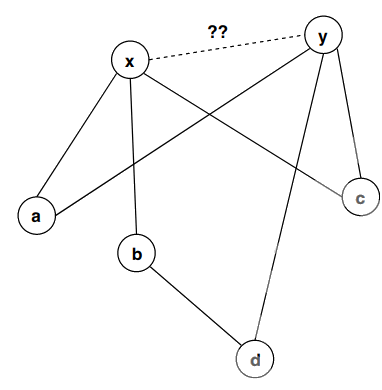
\includegraphics[width=7cm, keepaspectratio]{capitoli/methods/imgs/img6.png}
    \caption{An example illustrating the cycle formation link probability model.}
\end{figure}

Consider a cycle formation model ( \(CF (k)\) ) of degree \((k = 3)\).
The Seed link \((x, y)\), here, can be generated by the following three
mechanisms: - \texttt{random\ link\ occurrence\ g(1)} -
\texttt{length-2\ cycle\ generation\ g(2)}
i.e.~\((x −a −y and x −c −y)\) -
\texttt{length-4\ cycle\ generation\ g(3)} i.e.~\((x −b −d −y)\).

The main issue is to combine several generation mechanisms to compute
total link occurrence probability. The author posits a method to combine
both path and cycle (of different lengths) generation mechanism in the
framework. The expected general clustering coefficient of degree \(k\)
for this model can be estimated as
\[E[C(k)] = f(c_1, c_2, ..., c_k) = \sum_{i} |G_i|p(G_i)p((e_{l, k+1} \in E|G_i)) \]
where \(|G_i|\) is the number of subgraph possible corresponding to the
graph pattern \(G_i\), \(p(G_i)\) is the probability of occurrence of
one of such graphs \(G_i\), and \(p(e_{l,k+l})\) is the probability of
edge \(e_{l,l+1}\) to occur given the pattern \(G_i\). Finally, given
the coefficients, the probability of existence of link is
\[p_{x,y}(c_1, ..., c_k) = \frac{c_1 \prod_{i=2}^{k} c_i^{|path^i_{x,y}|}}{c_1 \prod_{i=2}^{k} c_i^{|path^i_{x,y}|} + (1-c_1)\prod_{i=2}^{k} (1-c_i)^{|path^i_{x,y}|}}\]

\textbf{Liu et al.} proposed degree related clustering coefficient to
quantify the clustering ability of nodes. They applied the same to paths
of shorter lengths and introduced a new index
\texttt{Degree\ related\ Clustering\ ability\ Path\ (DCP)}. They
performed the \texttt{degree\ of\ robustness\ (DR)} test for their index
and showed that missing links have a small effect on the index. Recently
\textbf{Wu et al.} extracted triangle structure information in the form
of node clustering coefficient of common neighbors. Their experiments on
several real datasets show comparable results to the \texttt{CAR} index.
The same concept of the clustering coefficient also introduced in the
work presented by \textbf{Wu et al.}. Authors introduce both node and
link clustering information in their work. Their experiments on
different network datasets showed better performance results against
existing methods, especially on middle and large network datasets.
\textbf{Kumar et al.} explored the concept of node clustering
coefficient to the next level (level-2) that captures more clustering
information of a network. The comprehensive results on several
real-world datasets show better performance compared to local methods
and comparable to the node embedding method \texttt{Node2vec}.
Meanwhile, \textbf{Benson et al.} studied simplicial closure events to
capture higher-order structures in several temporal networks. The
simplicial closure events are the process of closure of timestamped
simplices (simplicial complexes 2 are set of nodes with different sizes)
available in a dataset. These structures are common in several real-time
complex systems, for example, communication in a group, collaboration of
authors for a paper, etc. To assess these higher-order structures, the
authors study the simplicial closure events on triples of nodes (for
simplicity) and suggest that the open triangles or triples of nodes with
strong ties are more likely to close in the future.

\subsection{Structural Perturbation Method}

\textbf{\emph{Lu et al.}} introduced a new framework of computing
predictability of links in the networks. They coined a
\textbf{structural consistency index} to quantify the link
predictability. This index is based on the assumption that ``\emph{links
    in a network are highly predictable if no significant changes occur in
    the structural feature after the addition or deletion of a small
    fraction of the link}''. Based on this index, they proposed a new
similarity index, namely
\texttt{structural\ perturbation\ method\ (SPM)}. The experimental
results show the outstanding performance compared to the
state-of-the-art in their paper.

\chapter{Existing Methods \normalfont{\emoji{bookmark-tabs}}}

Recently, numerous methodologies of link prediction have been
implemented. These methods can be grouped into several categories, like
\textbf{similarity-based, probabilistic models, learning-based models},
etc.

\begin{figure}[H]
    \centering
    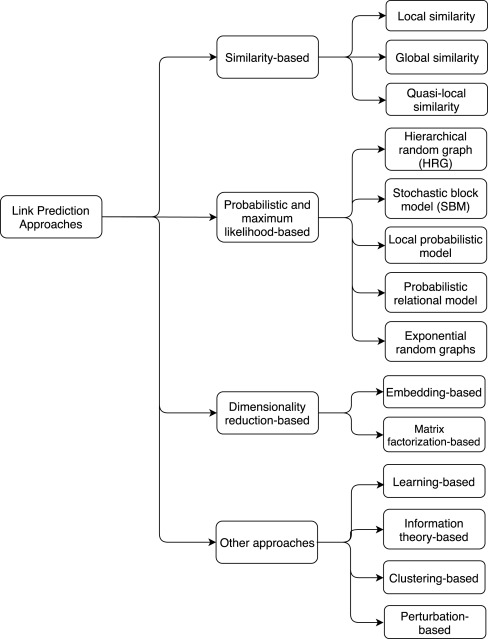
\includegraphics[width=9cm, keepaspectratio]{capitoli/methods/imgs/img2.jpg}
\end{figure}

\section{Similarity-based Methods}

Similarity-based metrics are the simplest one in link prediction, in
which for each pair \(x\) and \(y\), a similarity score \(S(x, y)\) is
calculated. The score \(S(x, y)\) is based on the structural or node's
properties of the considered pair. The non-observed links (i.e.,
\(U - E^T\) ) are assigned scores according to their similarities.
\textbf{The pair of nodes having a higher score represents the predicted
    link between them}. The similarity measures between every pair \emph{can
    be calculated using several properties of the network}, one of which is
structural property. Scores based on this property can be grouped in
several categories like \textbf{local and global}, and so on.

\subsection{Local similarity indices}

Local indices are generally calculated using information about common
neighbors and node degree. These indices \textbf{consider immediate
    neighbors of a node}. The following are some examples of local
similarity indices with a description and method to calculate them:

\begin{itemize}
    \item \texttt{Common\ Neighbors\ (CN)}: In a given network or graph, the size
          of common neighbors for a given pair of nodes \(x\) and \(y\) is
          calculated as the size of the intersection of the two nodes
          neighborhoods ( \(\Gamma\) ). \[S(x, y) = |\Gamma(x) \cap \Gamma(y)|\]
          The likelihood of the existence of a link between x and y increases with
          the number of common neighbors between them.
    \item \texttt{Jaccard\ Coefficient}: This metric is similar to the Common
          Neighbors. Additionally, it normalizes the above score, as given below:
          \[S(x, y) = \frac{|\Gamma(x) \cap \Gamma(y)|}{|\Gamma(x) \cup \Gamma(y)|}\]
          The Jaccard coefficient is defined as the probability of selection of
          common neighbors of pairwise vertices from all the neighbors of either
          vertex. The pairwise Jaccard score increases with the number of common
          neighbors between the two vertices considered. Some researcher
          (\textbf{Liben-Nowell et al.}) demonstrated that this similarity metric
          \textbf{performs worse} as compared to Common Neighbors.
    \item \texttt{Adamic/Adar\ Index\ (AA)}: Adamic and Adar presented a metric to
          calculate a similarity score between two web pages based on shared
          features, which are further used in link prediction after some
          modification
          \[S(x, y) = \sum_{z \in \Gamma(x) \cap \Gamma(y)} \frac{1}{log k_z}\]
          where \(k_z\) is the degree of the node \(z\). It is clear from the
          equation that more weights are assigned to the common neighbors having
          smaller degrees. This is also intuitive in the real-world scenario, for
          example, a person with more number of friends spend less time/resource
          with an individual friend as compared to the less number of friends.
    \item \texttt{Preferential\ Attachment\ (PA)}: The idea of preferential
          attachment is applied to generate a growing scale-free network. The term
          \textbf{growing} represents the incremental nature of nodes over time in
          the network. The likelihood incrementing new connection associated with
          a node \(x\) is proportional to \(k_x\) , the degree of the node.
          Preferential attachment score between two nodes x and y can be computed
          as: \[S(x, y) = k_x k_y\] This index shows the worst performance on most
          networks. The \textbf{simplicity} (as it requires the least information
          for the score calculation) and the \textbf{computational time} of this
          metric are the main advantages. PA shows better results if larger degree
          nodes are densely connected, and lower degree nodes are rarely
          connected. In the above equation, summation can also be used instead of
          multiplication as an aggregate function.
    \item \texttt{Resource\ Allocation\ Index\ (RA)}: Consider two non-adjacent
          vertices \(x\) and \(y\). Suppose node \(x\) sends some resources to
          \(y\) through the common nodes of both \(x\) and \(y\) then the
          similarity between the two vertices is computed in terms of
          \textbf{resources sent} from \(x\) to \(y\). This is expressed
          mathematically as:
          \[S(x, y) = \sum_{z \in \Gamma(x) \cap \Gamma(y)} \frac{1}{k_z}\] The
          difference between \textbf{RA} and \textbf{AA} is that the RA index
          heavily penalizes to higher degree nodes compared to the AA index.
          Prediction results of these indices become almost the same for smaller
          average degree networks. This index shows good performance on
          heterogeneous networks with a high clustering coefficient, especially on
          transportation networks.
    \item \texttt{Cosine\ similarity\ or\ Salton\ Index\ (SI)}: This similarity
          index between two records (documents) is measured by calculating the
          Cosine of the angle between them. The metric is all about the
          orientation and not magnitude. The Cosine similarity can be computed as
          \[S(x, y) = \frac{|\Gamma(x) \cap \Gamma(y)|}{\sqrt{(k_x k_y)}}\] -
          \texttt{Sorensen\ Index}: It is very similar to the Jaccard index.
          \textbf{McCune et al.} show that it \textbf{is more robust than Jaccard
              against the outliers}.
          \[S(x, y) = \frac{2|\Gamma(x) \cap \Gamma(y)|}{k_X + k_y}\]
    \item \texttt{CAR-based\ Common\ Neighbor\ Index\ (CAR)}: CAR-based indices
          are presented based on the assumption that the link existence between
          two nodes is more likely if their common neighbors are members of a
          local community (local-community-paradigm (LCP) theory). In other words,
          the likelihood existence increases with the number of links among the
          common neighbors (local community links (LCLs)) of the seed node pair as
          described in the following figure.
          \[S(x, y) = CN(x, y) \text{ x } LCL(x, y) = CN(x, y) \text{ x } \sum_{z \in \Gamma(x) \cap \Gamma(y)} \frac{|\gamma(z)|}{2} \]
          where \(CN(x, y) = |\Gamma(x) ∩ \Gamma(y)|\) is number of common
          neighbors. \(LCL(x, y)\) refers to the number of local community links
          which are defined as the links among the common neighbors of seed nodes
          x and y. \(\gamma(z)\) is the subset of neighbors of node \(z\) that are
          also common neighbors of \(x\) and \(y\).

          \begin{figure}[H]
              \centering
              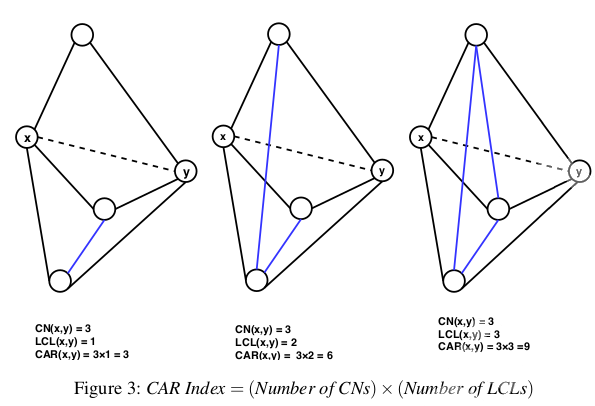
\includegraphics[width=8cm, keepaspectratio]{capitoli/methods/imgs/img3.png}
          \end{figure}
    \item \texttt{CAR-based\ Adamic/Adar\ Index\ (CAA)}: If \(LCL\) is considered
          as an accuracy enhancer, then the \(CAA\) index is obtained by
          incorporating the \(LCL\) theory to the well known AA index and
          mathematically expressed by the equation given below.
          \[S(x, y) = \sum_{z \in \Gamma(x) \cap \Gamma(y)} \frac{|\gamma(z)|}{\log_2(k_z)} \]
    \item \texttt{CAR-based\ Resource\ Allocation\ Index\ (CRA)}: Is a general
          application of the LCL theory to other indices and generate the CRA
          index by incorporating this concept into the existing RA index of the
          literature. Mathematically, the CRA can be expressed as
          \[S(x, y) = \sum_{z \in \Gamma(x) \cap \Gamma(y)} \frac{|\gamma(z)|}{k_z}\]
    \item \texttt{CAR-based\ Preferential\ Attachment\ Index\ (CPA)}: This is
          the preferential attachment index based on the CAR index. CPA is
          obtained by incorporating the LCL theory to the original PA method and
          expressed mathematically by
          \[S(x, y) = e_x e_y + e_x CAR(x, y) + e_y CAR(x, y) + CAR(x, y)^2\]
          where \(e_x\) is the number of neighbors of \(x\) not shared by \(y\)
          and \(CAR(x, y)\) is the similarity score of the node pair \(x\) and
          \(y\) using CAR index. CAR-based methods listed above show the best
          performance on LCP networks. The LCP networks are related to dynamic and
          heterogeneous systems and facilitate network evolution of social and
          biological networks.
    \item \texttt{Hub\ Promoted\ Index\ (HPI)}: This
          similarity index promotes the formation of links between the sparsely
          connected nodes and hubs. It also tries to prevent links formation
          between the hub nodes. This similarity metric can be expressed
          mathematically as
          \[S(x, y) = \frac{|\Gamma(x) \cap \Gamma(y)|}{min(k_x, k_y)}\]
    \item \texttt{Hub\ Depressed\ Index\ (HDI)}: This index is the same as the
          previous one but with the opposite goal as it avoids the formation of
          links between hubs and low degree nodes in the networks. The Hub
          depressed index promotes the links evolution between the hubs as well as
          the low degree nodes. The mathematical expression for this index is
          given below.
          \[S(x, y) = \frac{|\Gamma(x) \cap \Gamma(y)|}{max(k_x, k_y)}\]
    \item \texttt{Local\ Naive\ Bayes-based\ Common\ Neighbors\ (LNBCN)}: The
          above similarity indices are somehow based on common neighbors of the
          node pair where each of the which are equally weighted. This method is
          based on the Naive Bayes theory and arguments that different common
          neighbors play different role in the network and hence contributes
          differently to the score function computed for non-observed node pairs
          \[S(x, y) = \sum_{z \in \Gamma(x) \cap \Gamma(y)} [log(\frac{C(z)}{1 - C(z)}) + log(\frac{1 - \rho}{\rho})]\]
          where \(C(z)\) is node clustering coefficient and \(\rho\) is the
          network density expressed as \[\rho = \frac{|E|}{n(n-1)/2}\]
    \item \texttt{Leicht-Holme-Newman\ Local\ Index\ (LHNL)}: The logic below this
          index is that two vertices are similar to each other if their
          corresponding neighbors are self-similar to themselves. This score is
          defined by the ratio of the path of length two that exits between two
          vertices and the expected path of the same length between them.
          \[S(x, y) = \frac{|\Gamma(x) \cap \Gamma(y)|}{k_x k_y}\]
    \item \texttt{Node\ Clustering\ Coefficient\ (CCLP)}: This index is also based
          on the clustering coefficient property of the network in which the
          clustering coefficients of all the common neighbors of a seed node pair
          are computed and summed to find the final similarity score of the pair.
          Mathematically \[S(x, y) = \sum_{z \in \Gamma(x) \cap \Gamma(y)} C(z)\]
          where \[C(z) = \frac{t(z)}{k_z(k_z - 1)}\] is clustering coefficient of
          the node \(z\) and \(t(z)\) is the total triangles passing through the
          node \(z\).
    \item \texttt{Node\ and\ Link\ Clustering\ coefficient\ (NLC)}:
          This similarity index is based on the basic topological feature of a
          network called ''\emph{Clustering Coefficient}''. The clustering
          coefficients of both nodes and links are incorporated to compute the
          similarity score.
          \[S(x, y) = \sum_{z \in \Gamma(x) \cap \Gamma(y)} \frac{|\Gamma(x) \cap \Gamma(z)|}{k_z -1} \text{ x }C(z) + \frac{|\Gamma(y) \cap \Gamma(z)|}{k_z -1} \text{ x }C(z)\]

\end{itemize}

\subsection{Global similarity indices}

Global indices are computed using entire topological information of a
network. The computational complexities of such methods are higher and
seem to be infeasible for large networks.

\begin{itemize}
    \item \texttt{Katz\ Index}: This
          index can be considered as a variant of the shortest path metric. It
          directly aggregates over all the paths between x and y and dumps
          exponentially for longer paths to penalize them. It can be expressed
          mathematically as:
          \[S(x, y) = \sum_{l = 1}^{\infty}\beta^l|paths_{x, y}^{<l>}| = \sum_{l = 1}^{\infty}\beta^l(A)^l_{x, y}\]
          where, \(paths_{x, y}^{<l>}\) is considered as the set of total \(l\)
          length paths between \(x\) and \(y\), \(\beta\) is a damping factor that
          controls the path weights and A is the adjacency matrix. For the
          convergence of above equation, \[\beta < \frac{1}{\lambda_1} \] where
          \(\lambda_1\) is the maximum eigenvalue of the matrix A. If 1 is added
          to each element of the diagonal of the resulting similarity matrix S,
          this expression can be written in matrix terms as \[S = \beta AS + I\]
          where \(I\) is the identity matrix of the proper dimension. The
          similarity between all pairs of nodes can be directly computed using the
          closed-form by rearranging for \(S\) in the previous expression and
          subtracting the previously added 1 to the elements in the diagonal. Katz
          score for each pair of nodes in the network is calculated by finding the
          similarity matrix as \[S = (I - \beta A)^{- 1} - I\] The computational
          complexity of the given metric is high, and it can be roughly estimated
          to be cubic complexity which is not feasible for a large network.
    \item \texttt{Random\ Walk\ with\ Restart\ (RWR)}: Let \(\alpha\) be a
          probability that a random walker iteratively moves to an arbitrary
          neighbor and returns to the same starting vertex with probability
          \((1 - \alpha)\). Consider \(q_{xy}\) to be the probability that a
          random walker who starts walking from vertex \(x\) and located at the
          vertex \(y\) in steady-state. Now, this probability of walker to reach
          the vertex \(y\) is expressed mathematically as
          \[\overrightarrow{q_x} = \alpha P^T \overrightarrow{q_x} + (1-\alpha) \overrightarrow{e_x}\]
          where \(\overrightarrow{e_x}\) is the seed vector of length \(|V|\)
          (i.e., the total number of vertices in the graph). This vector consists
          of zeros for all components except the elements \(x\) itself. The
          transition matrix \(P\) can be expressed as
          \[\overrightarrow{q_x} = (1-\alpha)(I - \alpha P^T)^{-1} \overrightarrow{e_x}\]
          Since this similarity is not symmetric, the final score between the node
          pair (x, y) can be computed as \[S(x, y) = q_{xy} + q_{yx}\] It is clear
          from the above equation that matrix inversion is required to solve,
          which is quite expensive and prohibitive for large networks.
    \item \texttt{Shortest\ Path}: The inverse relation between the similarity and
          length of the shortest path is captured by the following mathematical
          equation given below. \[S(x, y) = -|d(x, y)|\] where Dijkstra algorithm
          is applied to efficiently compute the shortest path d(x, y) between the
          node pair (x, y). The prediction accuracy of this index is low compared
          to most local indices.
    \item \texttt{Leicht-Holme-Newman\ Global\ Index\ (LHNG)}: This global index
          is based on the principle that two nodes are similar if either of them
          has an immediate neighbor, which is similar to the other node. This is a
          recursive definition of similarity where a termination condition is
          needed. The termination condition is introduced in terms of
          self-similarity, i.e., a node is similar to itself. Thus, the similarity
          score equation consists of two terms: first, the neighbor similarity,
          and the second, self-similarity, as given below.
          \[S(x, y) = \phi  \sum_z A_{x, z} S_{z, y} + \psi \delta_{x, y}\] Here,
          the first term is neighborhood similarity and the second term is
          self-similarity. \(\psi\) and \(\phi\) are free parameters that make a
          balance between these two terms. When the free parameter \(\psi\) = 1,
          this index resembles to the Katz index.
    \item \texttt{Cosine\ based\ on\ L+\ (Cos+)}: Laplacian matrix is extensively
          used as an alternative representation of graphs in spectral graph
          theory. This matrix can be defined as \(L = D - A\), where, \(D\) is the
          diagonal matrix consisting of the degrees of each node of the matrix and
          \(A\) is the adjacency matrix of the graph. The pseudo-inverse of the
          matrix defined by Moore-Penrose is represented as \(L^+\) and each entry
          of this matrix is used to represent the similarity score between the two
          corresponding nodes. The most common way to compute this pseudo-inverse
          is by computing the \textbf{singular value decomposition (SVD)} of the
          Laplacian matrix [$(L = U \Sigma V^{}T)$, where \(U\) and \(V\)
                  are left and right singular vectors of \(SVD\)] as follows
          \[L^+ = V \Sigma^+ U^T\] \(\Sigma^+\) is obtained by taking the inverse
          of each nonzero element of the \(\Sigma\). Further, the similarity
          between two nodes \(x\) and \(y\) can be computed using any inner
          product measure such as Cosine similarity given as
          \[S(x, y) = \frac{L_{x, y}^+}{\sqrt{L_{x, x}^+ L_{y, y}^+}}\]
    \item \texttt{Average\ Commute\ Time\ (ACT)}: This index is based on the
          random walk concept. A random walk is a Markov chain which describes the
          movements of a walker. It defined as the average number of
          movements/steps required by a random walker to reach the destination
          node \(y\), and come back to the starting node \(x\). If \(m(x, y)\) be
          the number of steps required by the walker to reach \(y\) from \(x\),
          then the following expression captures this concept.
          \[n(x, y) = |E| (l_{xx}^+ + l_{yy}^+ - 2l_{xy}^+) \] where \(l_{xy}^+\)
          denotes the \((x, y)\) entry of the matrix \(L^+\) . Pseudo-inverse of
          the Laplacian, \(L^+\) can be computed as
          \[L^+ = (L - \frac{ee^T}{n})^{-1} + \frac{ee^T}{n}\] where \(e\) is a
          column vector consisting of 1's. Smaller value of this equation will
          represent higher similarity. The final expression is the following
          \[S(x, y) = \frac{1}{l_{xx}^+ + l_{yy}^+ - 2l_{xy}^+}\]
    \item \texttt{Normalized\ Average\ Commute\ Time\ (NACT)}: This is a variant
          of ACT that takes into account node degrees. For a high degree node
          (hub) \(y\), \(m(x, y)\) is usually small regardless of \(x\), the
          similarity measure is normalized with stationary distribution \(\pi\) of
          the Markov chain describing random walker on the graph. This normalized
          measure can be computed with the following equation
          \[S(x, y) = \frac{1}{(m(x, y)\pi_y + m(y, x)\pi_x)}\]
    \item \texttt{Matrix\ Forest\ Index\ (MF)}: his index is based on the concept
          of spanning tree which is defined as the subgraph that spans total nodes
          without forming any cycle. The spanning tree may contain total or less
          number of links as compared to the original graph. Chebotarev and Shamis
          proposed a theorem called matrix-forest theorem which states that the
          number of spanning tree in a graph is equal to the co-factor of any
          entry of Laplacian matrix of the graph. Here, the term forest represents
          the union of all rooted disjoint spanning trees. The similarity between
          two nodes \(x\) and \(y\) can be computed with the equation given below
          \[S = (I + L)^{-1}\] where \((I + L)\_{(x,y)}\) is the number of
          spanning rooted forests ( \(x\) as root ) consisting of both the nodes
          \(x\) and \(y\). Moreover, this quantity is equal to the co-factor of
          \((I + L)_{(x,y)}\) .
    \item \texttt{SimRank}: This is a measure of
          structural context similarity and shows object-to-object relationships.
          It is not domain-specific and recommends to apply in directed or mixed
          networks. The basic assumption of this measure is that two objects are
          similar if they are related to similar objects. SimRank computes how
          soon two random walkers meet each other, starting from two different
          positions. This measure can be represented in matrix form as
          \[S(x,y) = \alpha W^T SW + (1 - \alpha)I\] where, \(\alpha \in (0, 1)\)
          is a constant. \(W\) is the transformation matrix and computed by
          normalizing each column of adjacency matrix \(A\) as
          \[
              W_{ij} = \frac{a_{ij}}{\sum_{k=1}^{n}}
          \]
          The computational complexity
          of this measure is high for a large network, and to reduce its time, the
          authors suggest pruning recursive branches.
    \item \texttt{Rooted\ Pagerank\ (RPR)}: The idea of PageRank was originally
          proposed to rank the web pages based on the importance of those pages.
          The algorithm is based on the assumption that a random walker randomly
          goes to a web page with probability \(\alpha\) and follows hyper-link
          embedded in the page with probability \((1 - \alpha)\). Chung et
          al.~used this concept incorporated with a random walk in link prediction
          framework. The importance of web pages, in a random walk, can be
          replaced by stationary distribution. The similarity between two vertices
          \(x\) and \(y\) can be measured by the stationary probability of \(y\)
          from \(x\) in a random walk where the walker moves to an arbitrary
          neighboring vertex with probability \(\alpha\) and returns to \(x\) with
          probability \((1 - \alpha)\). Mathematically, this score can be computed
          for all pair of vertices as
          \[RPR = (1 - \alpha)(I - \alpha \hat{N})^{-1}\] where
          \(\hat{N} = D^{-1} A\) is the normalized adjacency matrix with the
          diagonal degree matrix \(D[i, i] = \sum_j A[i, j]\).
\end{itemize}

\subsection{Quasi-local indices}

Quasi-local indices have been introduced as a trade-off between local
and global approaches or performance and complexity. These metrics are
as efficient to compute as local indices. Some of these indices extract
the entire topological information of the network. The time complexities
of these indices are still below compared to the global approaches.

\begin{itemize}
    \item \texttt{Local\ Path\ Index\ (LP)}: This metric has the intent to furnish
          a good trade-off between accuracy and computational complexity. The
          metric is expressed mathematically as \[S^{LP} = A^2 + \epsilon A^3\]
          where $\epsilon$ represents a free parameter. Clearly, the measurement
          converges to common neighbor when \(\epsilon = 0\). If there is no
          direct connection between \(x\) and \(y\), \((A^3)_{xy}\) is equated to
          the total different paths of length 3 between \(x\) and \(y\). The index
          can also be expanded to generalized form
          \[S^{LP} = A^2 + \epsilon A^3 + \epsilon^2 A^4 + ... + \epsilon^{(n−2)} A^n\]
          where \(n\) is the maximal order. Computing this index becomes more
          complicated with the increasing value of \(n\). The LP index outperforms
          the proximity-based indices, such as RA, AA, and CN.
    \item \texttt{Path\ of\ Length\ 3\ (L3)}: Georg Simmel, a German sociologist,
          first coined the concept ``triadic closure'' and made popular by Mark
          Granovetter in his work ``\emph{The Strength of Weak Ties}''. The
          authors proposed a similarity index in protein-protein interaction (PPI)
          network, called \textbf{\emph{path of length 3 (or L3)}} published in
          the Nature Communication. They experimentally show that the triadic
          closure principle (TCP) does not work well with PPI networks. They
          showed the paradoxical behavior of the TCP (i.e., the path of length 2),
          which does not follow the structural and evolutionary mechanism that
          governs protein interaction. The TCP predicts well to the interaction of
          self-interaction proteins (SIPs), which are very small (4\%) in PPI
          networks and fails in prediction between SIP and non SIP that amounts to
          96\%. They showed that the L3 index performs well in such conditions and
          give mathematical expression to compute this index as
          \[S(x, y) = \sum \frac{a_{x,u} a_{u,v} a_{v,y}}{k_u k_v}\]
    \item \texttt{Similarity\ based\ on\ Local\ Random\ Walk\ and\ Superposed\ Random\ Walk\ (LRW\ and\ SRW)}:
          This metric propose a new similarity measures by exploiting the random
          walk concept on graphs with limited walk steps. They defined node
          similarity based on random walks of lower computational complexity
          compared to the other random walk based methods. Given a random walker,
          starting from the node \(x\), the probability of reaching the random
          walker to the node \(y\) in \(t\) steps is
          \[\overrightarrow{\pi}\_x(t) = P^T \overrightarrow{\pi}\_x(t-1)\] where
          \(\overrightarrow{\pi}\_x(0)\) is a column vector with \(x^{th}\)
          element as 1 while others are 0's and \(P^T\) is the transpose of the
          transition probability matrix \(P\). \(P_{xy}\) entry of this matrix
          defines the probability of a random walker at node \(x\) will move to
          the next node \(y\). It is expressed as \(P_{xy} = \frac{a_{kx}}{k_x}\)
          , where \(a_{xy}\) is 1 when there is a link between \(x\) and \(y\) and
          0, otherwise. The authors computed the similarity score ( \(LRW\) )
          between two nodes based on the above concept as
          \[S^{LRW}(x, y) = \frac{k_x}{2|E|}\pi_{xy}(t) + \frac{k_y}{2|E|}\pi_{xy}(t)\]
          This similarity measure focus on only few steps covered by the random
          walker (hence quasi-local) and not the stationary state compared to
          other approaches. Random walk based methods suffer from the situation
          where a random walker moves far away with a certain probability from the
          target node whether the target node is closer or not. This is an obvious
          problem in social networks that show a high clustering index i.e.,
          clustering property of the social networks. This degrades the similarity
          score between the two nodes and results in low prediction accuracy. One
          way to counter this problem is that continuously release the walkers at
          the starting point, which results in a higher similarity between the
          target node and the nearby nodes. By superposing the contribution of
          each walker (walkers move independently), SRW is expressed as
          \[S^{SRW} (x, y) (t) = \sum_{l=1}^{t} S^{LRW} (l)\]
\end{itemize}

\subsection{Some Remarks}

Similarity-based approaches mostly focus on the structural properties of
the networks to compute the similarity score. \textbf{\emph{Local
        approaches}} consider, in general, neighborhood information (direct
neighbors or neighbors of neighbor), which take less time for
computation. This is the property that makes the local approaches
feasible for massive real-world network datasets. \textbf{\emph{Global
        approaches}} consider the entire structural information of the network;
that is why time required to capture this information is more than local
and quasi-local approaches. Also, sometimes, entire topological
information may not be available at the time of computation, especially
in a decentralized environment. So, parallelization over the global
approaches may not possible or very complex compared to the local and
quasi-local approaches. The performance or prediction accuracy of these
approaches (i.e., global approaches) is better compared to local and
quasi-local. \textbf{\emph{Quasi-local approaches}} extract more
structural information than local and somehow less information compared
to the global.


\section{Probabilistic and maximum likelihood models}

For a given network \(G(V, E)\), \textbf{\emph{the probabilistic model
        optimizes an objective function to set up a model that is composed of
        several parameters}}. Observed data of the given network can be
estimated by this model nicely. At that point, the likelihood of the
presence of a non-existing link \((i, j)\) is evaluated using
conditional probability \(P(A_{i j} = 1 | \Theta )\). Several
\texttt{probabilistic\ models} and \texttt{maximum\ likelihood\ models}
have been proposed in the literature to \textbf{infer missing links in
    the networks}.\\

\textbf{The probabilistic models normally require more information like
    node or edge attribute knowledge in addition to structural information}
Extracting these attribute information is not easy; moreover, the
parameter tuning is also a big deal in such models that limit their
applicability. \emph{Maximum likelihood methods are complex and
    time-consuming}, so these models are not suitable for real large
networks.

\subsection{Local probabilistic model for link prediction}

\textbf{Wang et al.} proposed a \texttt{local\ probabilistic\ model} for
link prediction in an \emph{undirected network}. They employed three
different types of features viz., topological, semantic, and
cooccurrence probability features extracted from different sources of
information.\\

They presented an idea of a central neighborhood set derived from the
local topology of the considered node-pair, which is relevant
information for the estimation of a link between them. They computed
non-derivable frequent itemsets (i.e., those itemsets whose occurrence
statistics can not be derived from other itemset patterns) from the
network events log data, which is further used as training data for the
model. An event corresponds to a publication of a paper (i.e., authors'
interactions in the paper is a an event, and a set of such events is the
event log) in the Coauthorship network. The model is shown in the
following Figure, which considers the approach described below.\\

First, the central neighborhood set between \(x\) and \(y\) is
calculated based on local event log data. One of the usual ways to find
the central neighborhood set is to find the \textbf{shortest path
    between two vertices of specified length}, and the vertices are lying on
this path can be included in the required set. There can be more than
one shortest path between two vertices, so more neighborhood sets can be
possible. Neighborhood sets of shorter lengths and more frequent
(frequency score is used when more shortest paths of the same length are
available) are chosen for the central neighborhood set. The authors
considered the shortest path up to length 4 since the nodes lying on the
shorter length path are more relevant.\\

In the second step, for a given central neighborhood set, non-derivable
frequent itemsets are used to learn the local probabilistic model.
\textbf{Calders et al.} proposed a depth-first search method to
calculate non-derivable itemsets and the same algorithm used by the
authors. Why non-derivable frequent itemsets? \textbf{Pavlov et al.}
first introduced the concept of frequent itemset to construct an
\texttt{MRF}. They argued that a \(K-itemset\) and its support
represents a \(K-way\) statistics, which can be viewed as a constraint
on the true underlying distribution that generates the data. Given a set
of itemset constraints, a maximum entropy distribution satisfying all
these constraints is selected as the estimate for the true underlying
distribution. This maximum entropy distribution is equivalent to an
\texttt{MRF}. Since the number formed links are very few compared to all
possible links in a sparse network, the authors used a support threshold
of one to extract all frequent itemsets. Theses extracted itemsets are
large in number that results in expensive learning for the \texttt{MRF}.
To reduce this cost, only non-derivable itemsets are extracted. They
find all such itemsets that lie entirely within the central neighborhood
set. Using these itemsets, a \texttt{Markov\ Random\ Field} is
\textbf{learned}.\\

In the last step, the \texttt{iterative\ scaling\ algorithm} is used to
learn a local \texttt{MRF} for the given central neighborhood set. This
process continues overall itemset constraints and continuously updates
the model until the model converges. Once the model learning process is
over, one can infer the co-occurrence probability by computing the
marginal probability over the constructed model. The
\texttt{Junction\ tree\ inference\ algorithm} is used to infer
co-occurrence probability. The algorithm to induce co-occurrence
probability feature for a pair of vertices can be found in
\href{https://static.aminer.org/pdf/PDF/000/303/209a_parameterized_probabilistic_model_of_network_evolution_for_supervised_link.pdf}{Local
    Probabilistic Models for Link Prediction}.

\subsection{Probabilistic relational model for link prediction (PRM)}

Existing works show that \textbf{node attributes play a significant role
    to improve the link prediction accuracy}. However, \textbf{no generic
    framework is available to incorporate node and link attributes} and
hence, not applicable to all scenarios. To this end, \textbf{the
    probabilistic model is a good and concrete solution that provides a
    systematic approach to incorporate both node and link attributes in the
    link prediction framework}. Pioneering works on \texttt{PRM} include
\textbf{Getoor et al.} study on directed networks, \textbf{Taskar et
    al.} study on undirected networks, \textbf{Jennifer Neville}
work on for both networks, etc. published in \texttt{JMLR} is based on
\texttt{Relational\ Bayesian\ network\ (RBN)} where relation links are
directed and published in NIPS is based on
\texttt{Relational\ Markov\ network\ (RMN)} where relational links are
undirected.\\

\texttt{PRM} was originally designed for attribute prediction in
relational data, and it later extended to link prediction task. The
authors employed the attribute prediction framework to link prediction.
This casting can be understood with the following example: - Consider
the problem of link prediction in a coauthorship network. Non-relational
frameworks of link prediction consider only one entity type
``\emph{person}'' as node and one relationship; however, relational
framework (\texttt{PRMs}) include more entity types like article,
conference venue, institution, etc. Each entity can have attributes like
a person (attributes: name, affiliation institute, status (student,
professor)), article (attributes: publication year, type (regular,
review)), etc. Several relational links may possible among these
entities like advisor-advisee/research scholar relation between two
persons, author relationship between person and paper entities, and
paper can be related to the conference venue with publish relationship.
Moreover, relationships (links) among these entities can also have
attributes viz., exists (if there is a link between the two involved
entities), or not-exist (no link between the involved entities). This
way, the link prediction can be reduced to an attribute prediction
framework/model.\\

During the model training, a single link graph is constructed that
incorporates above heterogeneous entities and relationships among them.
Model parameters are estimated discriminatively to maximize the
probability of the link existence and other parameters with the given
graph attribute information. The learned model is then applied using
probabilistic inference to predict missing links.\\

\subsection{Hierarchical structure model (HSM)}

These models are based on the assumption that the structures of many
real networks are hierarchically organized, where nodes are divided into
groups, which are further subdivided into subgroups and so forth over
multiple scales. Some representative work systematically encodes such
structures from network data to build a model that estimates model
parameters using statistical methods. These parameters are then used in
estimating the link formation probability of unobserved links.\\

Some studies suggest that many real networks, like biochemical networks
(protein interaction networks, metabolic networks, or genetic regulatory
networks), Internet domains, etc. are hierarchically structured. In
hierarchical networks, vertices are divided into groups, which are
further sub-divided into subgroups and so forth over multiple scales.
\textbf{Clauset et al.} proposed a probabilistic model that takes a
hierarchical structure of the network into account. The model infers
hierarchical information from the network data and further applies it to
predict missing links.\\

The hierarchical structures are represented using a tree (binary), or
dendrogram, where, the leaves (i.e., \(n\) ) represent the number of
total vertices in the network and each internal vertex out of (
\(n - 1\) ) corresponds to the group of vertices descended from it. Each
internal vertex \(r\) is associated with a probability \(p_r\) , then
the existing edge probability \(p_{xy}\) between two vertices \(x\) and
\(y\) is given by \(p_{xy} = p_r\) where, \(r\) is their lowest common
ancestor. The hierarchical random graph is then, represented by the
dendrogram \(D^{\star}\) with the set of probability \(\{ p_r \}\) as
\(\left( D^{\star},\{p_r\} \right)\). Now the learning task is to find
the hierarchical random graph(s) that best estimates the observed
real-world network data. Assuming all possible dendrograms to be equally
likely, Bayes theorem says that the probability of the dendrogram
\(\left(D^{\star}, \{p_r\} \right)\) that best estimates the data is
proportional to the posterior probability or likelihood, \(L\) from
which the model generates the observed network and our goal is to
maximize \(L\) . The likelihood of a hierarchical random graph
\(\left(D^{\star},\{p_r\} \right)\) is computed using the following
equation

\[
    L(D^{\star}, \{p_r\}) = \prod_{r \in D^{\star}} p_r^{E_r} (1-p_r)^{L_r R_r - Er},
\]

where \(L_r\) and \(R_r\) are the left and right subtree rooted at
\(r\), and \(E_r\) is the number of links in the network whose endpoints
have \(r\) as their lowest common ancestor in \(D^{\star}\) . The above
equation assumes the convention \(0^0 = 1\). For a given dendrogram
\(D^{\star}\) , it is easy to compute the probability \(p_r\) that
maximizes \(L(D^{\star}, \{p_r\})\) i.e.

\[
    \overline{p_r} = \frac{E_r}{L_r R_r}.
\]

This can be understood with the following example illustrated in the
next Figure. Now, this model can be used to estimate the missing links
of the network as follows. Sample a large number of dendrograms with
probability proportional to their likelihood. Then, compute the mean
connecting probability \(\overline{p_{xy}}\) of each nonexisting pair
\((x, y)\) by averaging the corresponding probability \(p_{xy}\) overall
sampled dendrograms. Sort these vertices pairs scores in descending
order and selects top-l links to be predicted.

\begin{figure}[H]
    \centering
    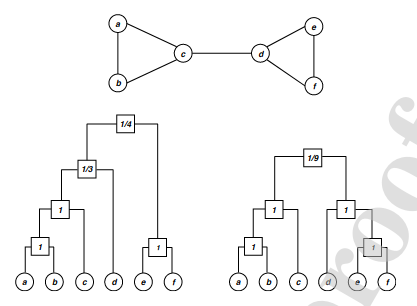
\includegraphics[width=8cm, keepaspectratio]{capitoli/methods/imgs/img8.png}
    \caption{ An illustrating example of \texttt{HSM} for a graph of 6 nodes and its
        two possible dendrograms. The internal nodes of each dendrogram are
        labeled as the maximum likelihood probability \(\overline{p}_r\). The
        likelihoods of the left and the right dendrograms are
        \(L(D1) = (1/3)(2/3)^2 (1/4)^2(3/4)^6\) \(= 0.00165\), and
        \(L(D2) = (1/9)(8/9)^8 = 0.0433\). Thus, the second (i.e., right)
        dendrogram is most probable as it divides the network in a balanced one
        at the first level.}
\end{figure}

\subsection{Stochastic block model (SMB)}

Hierarchical structures may not represent most networks. A more general
approach to represent these networks is block model where vertices are
distributed (partitioned) into blocks or communities and the connecting
probability between two vertices depends on blocks they belong to.
\textbf{Guimera et al.} presented a novel framework where stochastic
block model representation of a network is employed to find missing and
spurious links. The authors compute the reliability of the existence of
links given an observed network that is further used to find missing
links (non-existing links with higher reliabilities) and spurious links
(existing links with lower probabilities).\\

The link reliability \(R_{xy}\) between the two vertices \(x\) and \(y\)
is

\[R_{xy} = p_{BM} (A_{xy} = 1 | A^0).\]

i.e.~probability that the link truly exists given the observed network
\(A^0\), the block model \(BM\).\\

Generally, complex networks are outcomes of combination of mechanisms,
including modularity, role structure, and other factors. In \(SBM\),
partitioning vertices of network based on these mechanisms may result in
different block models that capture different correlations (patterns) of
the network. Assume that no prior knowledge of suitable models, the
reliability is expressed as

\[
    R_{xy} = \frac{1}{Z} \sum_{P \in P^{\star}} \left( \frac{l^{0}_{\sigma_x \sigma_y} + 1}{r^{0}_{\sigma_x \sigma_y + 2}} \right) \text{ exp } \left[ -H(P) \right],
\]

where the sum is over all possible partitions \(P^{\star}\) of the
network into groups, \(\sigma_x\) and \(\sigma_y\) are vertices \(x\)
and \(y\) groups in partition \(P\) respectively. Moreover, \(l^0_1\)
and \(r^0_{\sigma_{\alpha} \sigma_{\beta}}\) are the number of links and
maximum possible links in the observed network between groups \(\alpha\)
and \(\beta\) . The function \(H(P)\) is

\[H(P) = \sum_{\alpha \leq \beta} \left[ \ln \left( r_{\alpha \beta} \right) + \ln \binom {r_{\alpha \beta}}{l^0_{\alpha \beta}} \right],\]

and \(Z = \sum_{P \in P^{\star}} \text{ exp } \left[ -H(P) \right]\).\\

Practically, solving equation \(R_{xy} = \ldots\) , i.e., summing over
all possible partitions is too complex even for a small network.
However, the Metropolis algorithm can be used to correctly sample the
relevant partitions and obtain link reliability estimates.\\

The authors employed the link reliability concept to find missing links
and to identify the spurious link in the networks with the following
procedure.

\begin{itemize}
    \item
          \((i)\) Generate the observed network \(A^0\) by removing/adding some
          random links (for finding missing/spurious links) from/to the true
          network \(A^t\) .
    \item
          \((ii)\) Compute the link reliability for non-observed links (i.e.
          non-existing \(+\) missing/spurious links).
    \item
          \((iii)\) Arrange these links with their reliability score in
          decreasing order and decide the top-l links as desired ones (i.e.,
          missing/spurious links).
\end{itemize}

Probabilistic and maximum likelihood methods extract useful features and
valuable correlation among the data using hierarchical and stochastic
block models, which result in significant improvements in prediction
results as compared to some similarity-based methods. However, these are
\textbf{quite complex and time-consuming even on small datasets} that
limit their applicability on large scale real-world network datasets.

\subsection{Exponential random graph model (ERGM) or P-star model}

\section{Link prediction using Dimensionality Reduction}

The curse of dimensionality is a well-known problem in machine learning.
Some researchers employ dimension reduction techniques to tackle the
above problem and apply it in the \textbf{link prediction} scenario.

\subsection{Embedding-based link prediction}

The network embedding is considered as a dimensionality reduction
technique in which higher \(D\) dimensional nodes (vertices) in the
graphs are mapped to a lower \(d\) (\(d << D\)) \textbf{dimensional
    representation (embedding)} space by preserving the node neighborhood
structures. In other words, \textbf{\emph{find the embedding of nodes to
        a lower d-dimensions such that similar nodes (in the original network)
        have similar embedding (in the representation space)}}.\\ In the Figure
below you can see an application example of a dimensionality reduction
technique to a graph that represent a social network.

\begin{figure}[H]
    \centering
    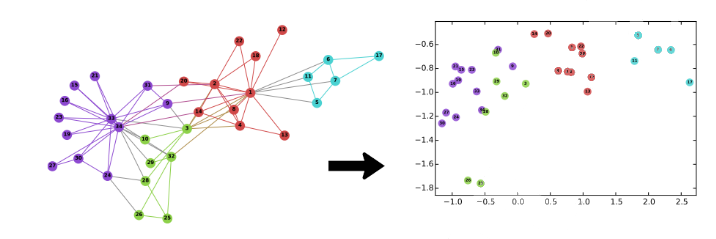
\includegraphics[width=12cm, keepaspectratio]{capitoli/methods/imgs/img4.png}
\end{figure}

The main component of the network embedding is the encoding function or
encoder \(f_{en}\) that map each node to the embedding space
\[f_{en}(x) = z_x\] where \(z_x\) is the \(d\)-dimensional embedding of
the node \(x\). The embedding matrix is \(Z \in R^{d x |V|}\), each
column of which represents an embedding vector of a node.\\

\begin{figure}[H]
    \centering
    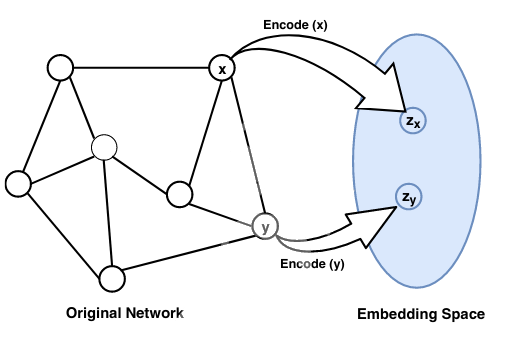
\includegraphics[width=10cm, keepaspectratio]{capitoli/methods/imgs/img5.png}
\end{figure}

Now, a similarity function is \(S(x, y)\) is defined that specifies how
to model the vector (embedding) space relationships equivalent to the
relationships in the original network, i.e.,
\[S(x, y) \approx z_x^T z_y\]

Here \(S(x, y)\) is the function that reconstructs pairwise similarity
values from the generated embedding. The term \(S(x, y)\) is the one
that differ according to the function used in different
factorization-based embedding approaches.\\

For example, \texttt{graph\ factorization} directly employ adjacency
matrix \(A\) i.e.~\((S(x, y) \overset{\Delta}{=} A_{(x,y)})\) to capture
first order proximity, \texttt{GraRep} selects
\((S(x, y) \overset{\Delta}{=} A^2_{(x,y)})\) and \texttt{HOPE} uses
other similarity measures(e.g. Jaccard neighborhood overlap). Most
embedding methods realize the reconstruction objective by minimizing the
loss function, L
\[L = \sum_{(x, y) \in \{V x V \}} l(z_x^T z_y, S(x, y))\]

Once the previous equation is \textbf{converged}
(i.e.~\textbf{trained}), one can use the trained encoder to generate
nodes embedding, which can further be employed to infer missing link and
other downstream machine learning tasks.\\

Recently, some network embedding techniques have been proposed and
applied successfully in link prediction problem. The
\texttt{Laplacian\ eigenmaps},
\texttt{Logically\ linear\ embedding\ (LLE)}, and \texttt{Isomap} are
examples based on the simple notion of embedding. Such embedding
techniques are having quite complex in nature and face scalability
issues. To tackle the scalability issue, graph embedding techniques have
leveraged the sparsity of real-world networks. For example,
\texttt{DeepWalk} extracts local information of truncated random walk
and embeds the nodes in representation space by considering the walk as
a sentence in the language model. It preserves higher order proximity by
maximizing the probability of co-occurrence of random walk of length
\(2k + 1\) (previous and next \(k\) nodes centered at a given node).
\texttt{Node2vec} also uses a random walk to preserves higher order
proximity but it is biased which is a trade-off between the
\texttt{breadth-first\ search\ (BFS)} and
\texttt{depth-first\ search\ (DFS)}.\\

The experimental results show that the \texttt{Node2vec} performs better
than the \texttt{Deepwalk}.\\

In next step, \textbf{Trouillon et al.} introduced complex embedding in
which simple matrix and tensor factorization have been used for link
prediction that uses a vector with complex values. Such composition of
complex embedding includes all possible binary relations especially
symmetric and anti-symmetric relations. Recently, some more studies have
been published in link prediction using embedding, for example,
\textbf{Cao et al.~subgraph embedding}, \textbf{Li et al.~deep dynamic
    network embedding}, \textbf{Kazemi et al.}, etc.

\subsection{Matrix factorization/decomposition-based link prediction}

From last decade, matrix factorization has been used in lots of papers
based on link prediction and recommendation systems. Typically, the
latent features are extracted and using these features, each vertex is
represented in latent space, and such representations are used in a
supervised or unsupervised framework for link prediction. To further
\textbf{improve the prediction results, some additional node/link or
    other attribute information can be used}. In most of the works,
non-negative matrix factorization has been used. Some authors also
applied the singular value decomposition technique. Let the input data
matrix is represented by \(X = (x_1, x_2, ..., x_n)\) that contains
\(n\) data vectors as columns. Now, factorization of this matrix can be
expressed as \[X \approx FG^T\] where
\(X \in R^{p x n}, F \in R^{p x k} , and G \in R^{n x k}\) . Here, \(F\)
contains the bases of the latent space and is called the basis matrix.
\(G\) contains combination of coefficients of the bases for
reconstructing the matrix \(X\) , and is called the coefficient matrix.
\(k\) is the dimension of latent space \((k < n)\). Several well-known
matrix factorizations are expressed based on some constraints on either
of the three matrices, for example

\begin{itemize}
    \item \texttt{SVD}:
          \(X_\pm \approx F_\pm G_\pm^T\)
    \item \texttt{NMF}:
          \(X_+ \approx F_+ G_+^T\)
    \item \texttt{Semi-NMF}:
          $X_\pm \approx F_\pm G_+\^{T} $
    \item \texttt{Convex-NMF}:
          $X_\pm \approx  X_\pm W_+ G_\pm^{T}$
\end{itemize}

In the above four equations, \(Z_\pm\) represents the nature of the
entries in the matrix \(Z\), i.e.~both positive and negative entries
allowed in the matrix \(Z\). In the last equation, \(F = XW\) represents
the convex combinations of the columns of \(F\) . Generally, such a
factorization problem can be modeled as the following
\texttt{Frobenius\ norm\ optimization\ problem}
\[min_{f, g} ||X - FG^T||^2_{fro}\]
\[\text{subject to} F \ge 0, G \ge 0\] Here \(||Z||^2_{fro}\) is the
frobenius norm of \(Z\) and the constraints represent NMF factorization.
However, any of the above four constraints can be used depending on the
requirement of the problem underlying. After solving the above
optimization problem, the similarity between a non-existing pair
\((x, y)\) can be computed by the similarity of the \(x^{th}\) and
\(y^{th}\) row vectors in the coefficient matrix \(G\).

\begin{itemize}
    % \tightlist
    \item
          \texttt{Acar\ et\ al.} expressed temporal link prediction as a matrix
          completion problem and solve it through the
          \texttt{matrix\ and\ tensor\ factorization}. They proposed a weighted
          method to collapsed the temporal data in a single matrix and factorize
          it using \texttt{CANDECOMP/PARAFAC\ (CP)} tensor decomposition method.
    \item
          \texttt{Ma\ et\ al.} also applied matrix factorization to temporal
          networks where features of each network are extracted using
          \texttt{graph\ communicability} and then collapsed into a single
          feature matrix using \texttt{weighted\ collapsing\ tensor\ (WCT)}.
          They showed the equivalence between eigen decomposition of
          \texttt{Katz\ matrix} and
          \texttt{non-negative\ matrix\ factorization\ (NMF)} of the
          communicability matrix that serves as the foundation of their
          framework.
    \item
          \texttt{Menon\ et\ al.} proposed a work for structural link
          prediction. Here, the problem is modeled as
          \texttt{matrix\ completion\ problem}, and
          \texttt{matrix\ factorization} are used to solve it. They introduced a
          supervised matrix decomposition framework that learns latent
          (unobserved) structural features of the graph and incorporates it with
          additional node/link explicit feature information to make a better
          prediction. Additionally, they allowed the factorization model to
          solve class imbalance problem by optimizing ranking loss.
    \item
          \texttt{Chen\ et\ al.} proposed a work, where the authors extracted
          topological matrix and attribute matrix and factorized these matrices
          using \texttt{non-negative\ matrix\ factorization}. The final score
          matrix is obtained by integrating these two matrices in the latent
          space.
\end{itemize}
\section{Other approaches}

\subsection{Learning-based frameworks for link prediction}

Earlier described approaches (e.g., similarity and probabilistic
methods) deal with the computing a score of each non-observed link
either by a similarity or a probabilistic function. However, \textbf{the
    link prediction problem can also be modeled as a learning-based model}
to exploit graph topological features and attribute information. The
problem is cast as a \textbf{supervised classification model} where a
\textbf{point} (i.e., training data) \textbf{corresponds to a
    vertex-pair in the network}, and the \textbf{label} of the point
\textbf{represents the presence or absence of an edge (link) between the
    pair}.\\ In other words, \emph{consider a vertex-pair} \(\mathit{(x, y)}\)
\emph{in the graph} \(\mathit{G(V, E)}\) \emph{and the label of the
    corresponding data point in the classification model is}
\(\mathit{l_{(x,y)}}\) . Then,

\[l_{(x, y)}=
    \begin{cases}
        +1 \ \text{ if } (x, y) \in E \\
        -1 \ \text{ if } (x, y) \notin E
    \end{cases}
\]

\textbf{This is typically a binary classification task} where several
classifiers (e.g.,
\texttt{decision\ tree,\ naive\ Bayes,\ support\ vector\ machine}, etc.)
can be employed to predict the label of unknown data points
(corresponding to missing links in the network). One of the major
challenges of this model (i.e., machine learning) is the
\textbf{selection of appropriate feature set}. Majority of the existing
research works extract feature sets from the network topology (i.e.,
topological information of the network). These \textbf{features are
    generic} and domain-independent that are \textbf{applicable to any
    network}. Such features are typical,
\texttt{neighborhood,\ and\ path-based\ features}.\\ Some other works
concentrate on extracting node and edge features that play a crucial
role to improve the performance of link prediction. The cost of
extraction of such features is cheap and easy, while the main
disadvantage is the domain-specific nature of them.

\subsection{Information theory-based link prediction}

Several complex networks have utilized the concept of
\textbf{information theory to compute their complexity on different
    scales}. They defined several correlation measures and modeled some
networks (e.g., \texttt{star,\ tree,\ lattice,\ ER\ graph}, etc.).
\textbf{Bauer et al.} used the \texttt{maximum\ entropy\ principle} to
assign a statistical weight to any graph and introduced random graph
construction with arbitrary degree distribution.\\

\textbf{Tan et al.} posed the link prediction problem in the
\texttt{framework\ of\ information\ theory}. They mainly focus on local
assortativity to capture local structural properties of the network and
showed that \texttt{mutual\ information\ (MI)} method performs well on
both low and highly correlated networks. Motivated by, \textbf{Zhu, B.
    and Xia} added more local features (i.e., links information of neighbors
of the seed nodes as well as their common neighbors) in their framework
and called it as \texttt{neighbor\ set\ information\ (NSI)\ index}.
Thus, they showed that the different features could be combined in an
information-theoretic model to improve the link prediction accuracy.\\

\textbf{Xu et al.} considered path entropy as a similarity metric for
the link prediction problem. The authors assumed that there is no
correlation among the degrees of the nodes in the network. Consider the
following notations based on their paper: \(L^0_{xy}\) shows no link
exists between two vertices \(x\) and \(y\), and the corresponding
existence is represented by \(L^1_{xy}\). Probability of existence of a
link between the above two vertices is given as

\[
    P(L^1_{xy}) = 1 - P(L^0_{xy}) = 1 - \frac{C^{k_y}_{M-k_x}}{C^{k_y}_M}
\]

where \(C_M^{k_Y}\) represents the number of candidate link sets for the
vertex \(y\) with all links incident with \(y\) and \(C^{k_y}_{M-k_x}\)
denotes the number of candidate link sets for the vertex \(y\) with all
links incident with \(y\) but none of them is incident with \(x\).
Outcome results on several networks demonstrate that the similarity
index based on path entropy performs better than other indices in terms
of prediction accuracy and precision. \textbf{Xu et al.} extend the
previous work to the weighted network by considering the weight of the
paths. Recently, some more efforts have been applied in this direction
based on different features of the networks like influential nodes,
combining node attributes with
\texttt{structural\ similarity,\ local\ likelihood,\ and\ maximal\ entropy\ random\ walk}.

\subsection{Clustering-based Link Prediction}

\textbf{Huang} presented a paper on
\texttt{graph\ topology-based\ link\ prediction} where a
\texttt{generalized\ clustering\ coefficient} is used as a
\textbf{predictive parameter}. The author introduces a \textbf{cycle
    formation model} that shows the relationship between link occurrence
probability and its ability to form different length cycles. This model
suggests that the occurrence probability of a particular link depends on
the number of different lengths cycles formed by adding this link. The
model is based on the assumption of the stationary property of the
degree of clustering of the network. This model captures longer cycles
by extending the higher-order clustering coefficients and defines the
generalized clustering coefficient \(C(k)\) as

\[C(k) = \frac{\textit{number of j-length cycles}}{\textit{number of k-length paths}}\]

where \(k\) is the \textbf{degree} of the cycle formation model.

The author treats the link occurrence probability as governed by \(t\)
link generation mechanisms \(g(1), g(2),...,g(k)\) of cycle formation
model, each described by a single parameter \(c_1, c_2,...,c_k\) . The
above mentioned link generation mechanism can be understood with the
help of the Figure below.

\begin{figure}[H]
    \centering
    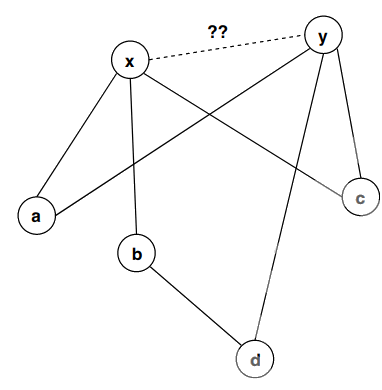
\includegraphics[width=7cm, keepaspectratio]{capitoli/methods/imgs/img6.png}
    \caption{An example illustrating the cycle formation link probability model.}
\end{figure}

Consider a cycle formation model ( \(CF (k)\) ) of degree \((k = 3)\).
The Seed link \((x, y)\), here, can be generated by the following three
mechanisms: - \texttt{random\ link\ occurrence\ g(1)} -
\texttt{length-2\ cycle\ generation\ g(2)}
i.e.~\((x −a −y and x −c −y)\) -
\texttt{length-4\ cycle\ generation\ g(3)} i.e.~\((x −b −d −y)\).

The main issue is to combine several generation mechanisms to compute
total link occurrence probability. The author posits a method to combine
both path and cycle (of different lengths) generation mechanism in the
framework. The expected general clustering coefficient of degree \(k\)
for this model can be estimated as
\[E[C(k)] = f(c_1, c_2, ..., c_k) = \sum_{i} |G_i|p(G_i)p((e_{l, k+1} \in E|G_i)) \]
where \(|G_i|\) is the number of subgraph possible corresponding to the
graph pattern \(G_i\), \(p(G_i)\) is the probability of occurrence of
one of such graphs \(G_i\), and \(p(e_{l,k+l})\) is the probability of
edge \(e_{l,l+1}\) to occur given the pattern \(G_i\). Finally, given
the coefficients, the probability of existence of link is
\[p_{x,y}(c_1, ..., c_k) = \frac{c_1 \prod_{i=2}^{k} c_i^{|path^i_{x,y}|}}{c_1 \prod_{i=2}^{k} c_i^{|path^i_{x,y}|} + (1-c_1)\prod_{i=2}^{k} (1-c_i)^{|path^i_{x,y}|}}\]

\textbf{Liu et al.} proposed degree related clustering coefficient to
quantify the clustering ability of nodes. They applied the same to paths
of shorter lengths and introduced a new index
\texttt{Degree\ related\ Clustering\ ability\ Path\ (DCP)}. They
performed the \texttt{degree\ of\ robustness\ (DR)} test for their index
and showed that missing links have a small effect on the index. Recently
\textbf{Wu et al.} extracted triangle structure information in the form
of node clustering coefficient of common neighbors. Their experiments on
several real datasets show comparable results to the \texttt{CAR} index.
The same concept of the clustering coefficient also introduced in the
work presented by \textbf{Wu et al.}. Authors introduce both node and
link clustering information in their work. Their experiments on
different network datasets showed better performance results against
existing methods, especially on middle and large network datasets.
\textbf{Kumar et al.} explored the concept of node clustering
coefficient to the next level (level-2) that captures more clustering
information of a network. The comprehensive results on several
real-world datasets show better performance compared to local methods
and comparable to the node embedding method \texttt{Node2vec}.
Meanwhile, \textbf{Benson et al.} studied simplicial closure events to
capture higher-order structures in several temporal networks. The
simplicial closure events are the process of closure of timestamped
simplices (simplicial complexes 2 are set of nodes with different sizes)
available in a dataset. These structures are common in several real-time
complex systems, for example, communication in a group, collaboration of
authors for a paper, etc. To assess these higher-order structures, the
authors study the simplicial closure events on triples of nodes (for
simplicity) and suggest that the open triangles or triples of nodes with
strong ties are more likely to close in the future.

\subsection{Structural Perturbation Method}

\textbf{\emph{Lu et al.}} introduced a new framework of computing
predictability of links in the networks. They coined a
\textbf{structural consistency index} to quantify the link
predictability. This index is based on the assumption that ``\emph{links
    in a network are highly predictable if no significant changes occur in
    the structural feature after the addition or deletion of a small
    fraction of the link}''. Based on this index, they proposed a new
similarity index, namely
\texttt{structural\ perturbation\ method\ (SPM)}. The experimental
results show the outstanding performance compared to the
state-of-the-art in their paper.



\end{document}